%%\clearpage
%%\subsection{Top control region}
%%\label{subsec:top_cr}

Figures
\ref{fig:CRTopResLoosePlots1Lep}
\ref{fig:CRTopResTightPlots1Lep}
\ref{fig:CRTopMerLPPlots1Lep}
\ref{fig:CRTopMerHPPlots1Lep}
show the main relevant kinematic variable distributions in the Top CR in \olep channel, after \mjjtag reweighting has been applied.

\begin{figure}[ht]
    \centering
    \subfloat[]{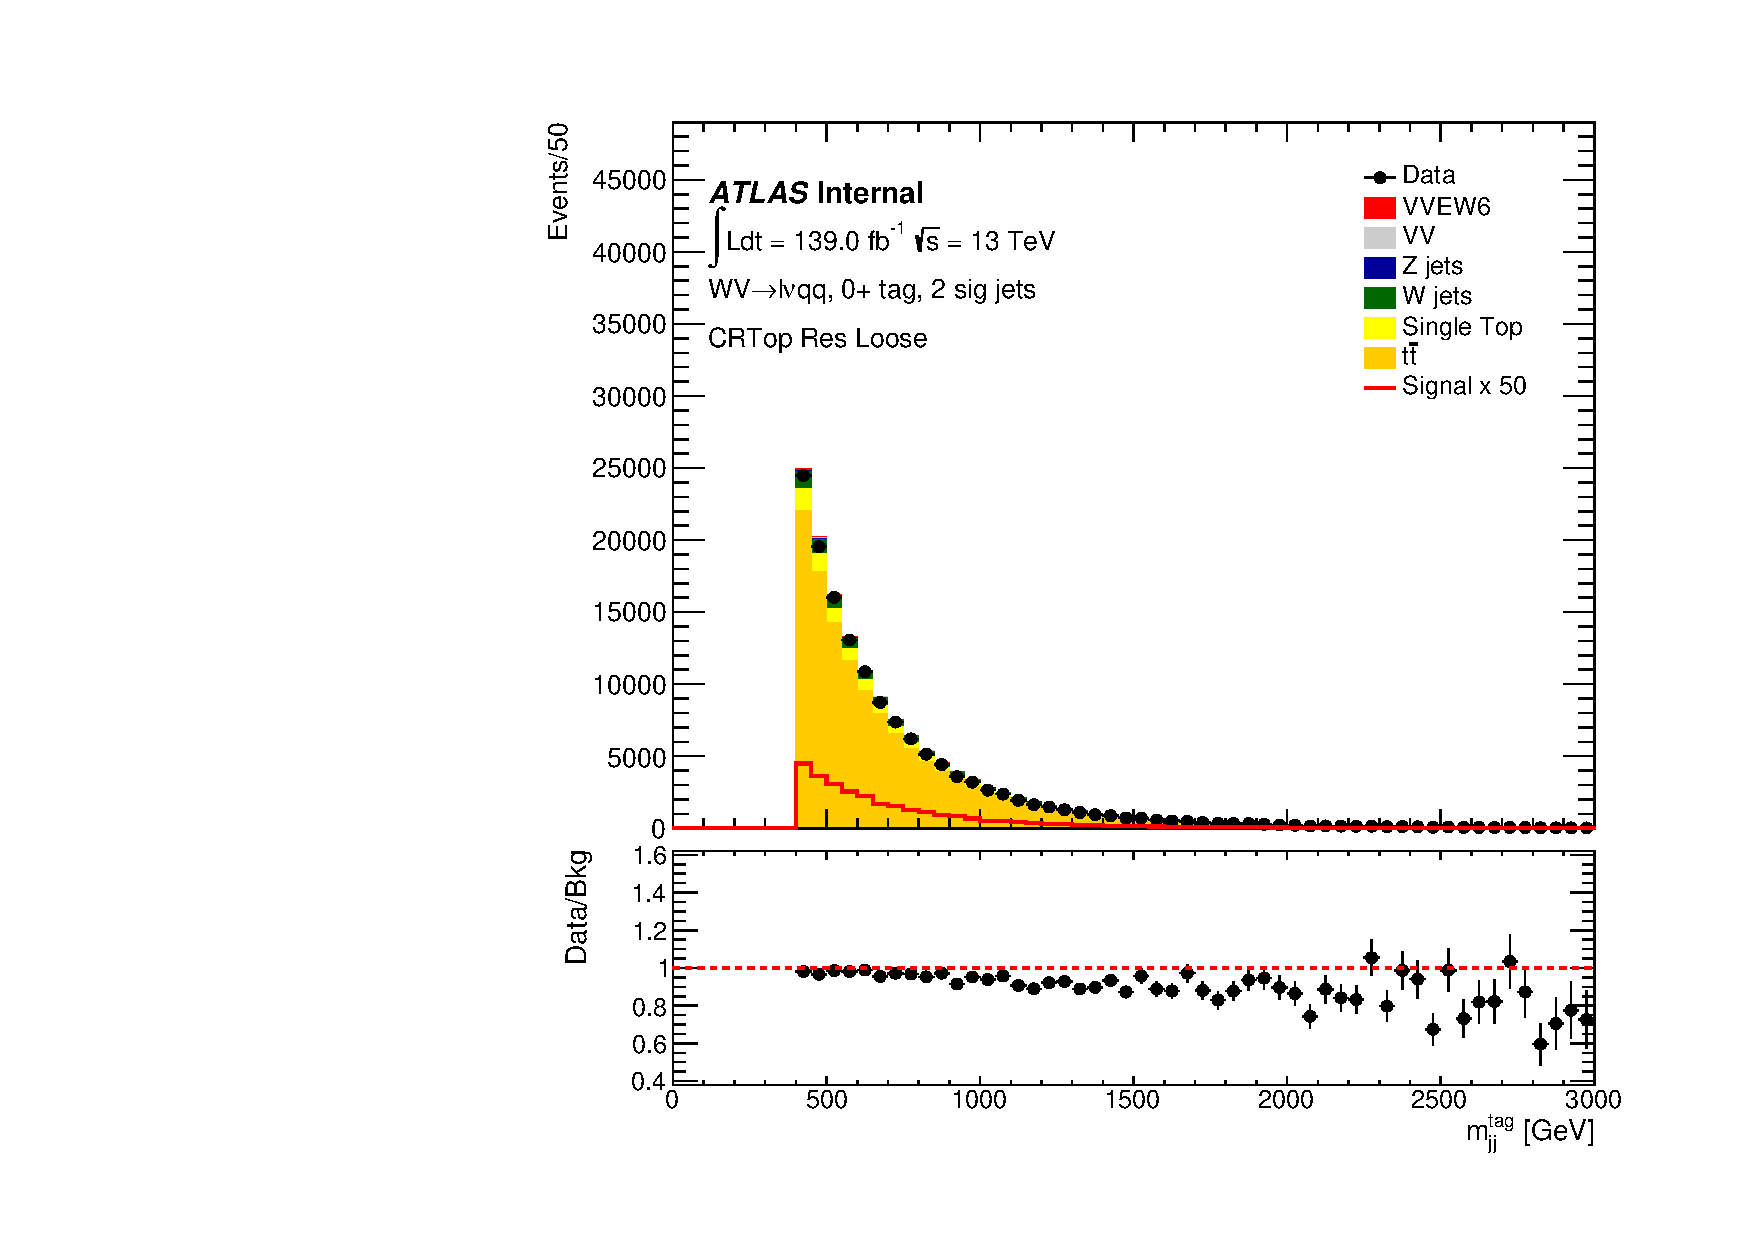
\includegraphics[width=0.3\textwidth]{figures/CRPlots/CRTop_Res_Loose/stacked_plot_resolved_tagMjj.pdf}}
    \subfloat[]{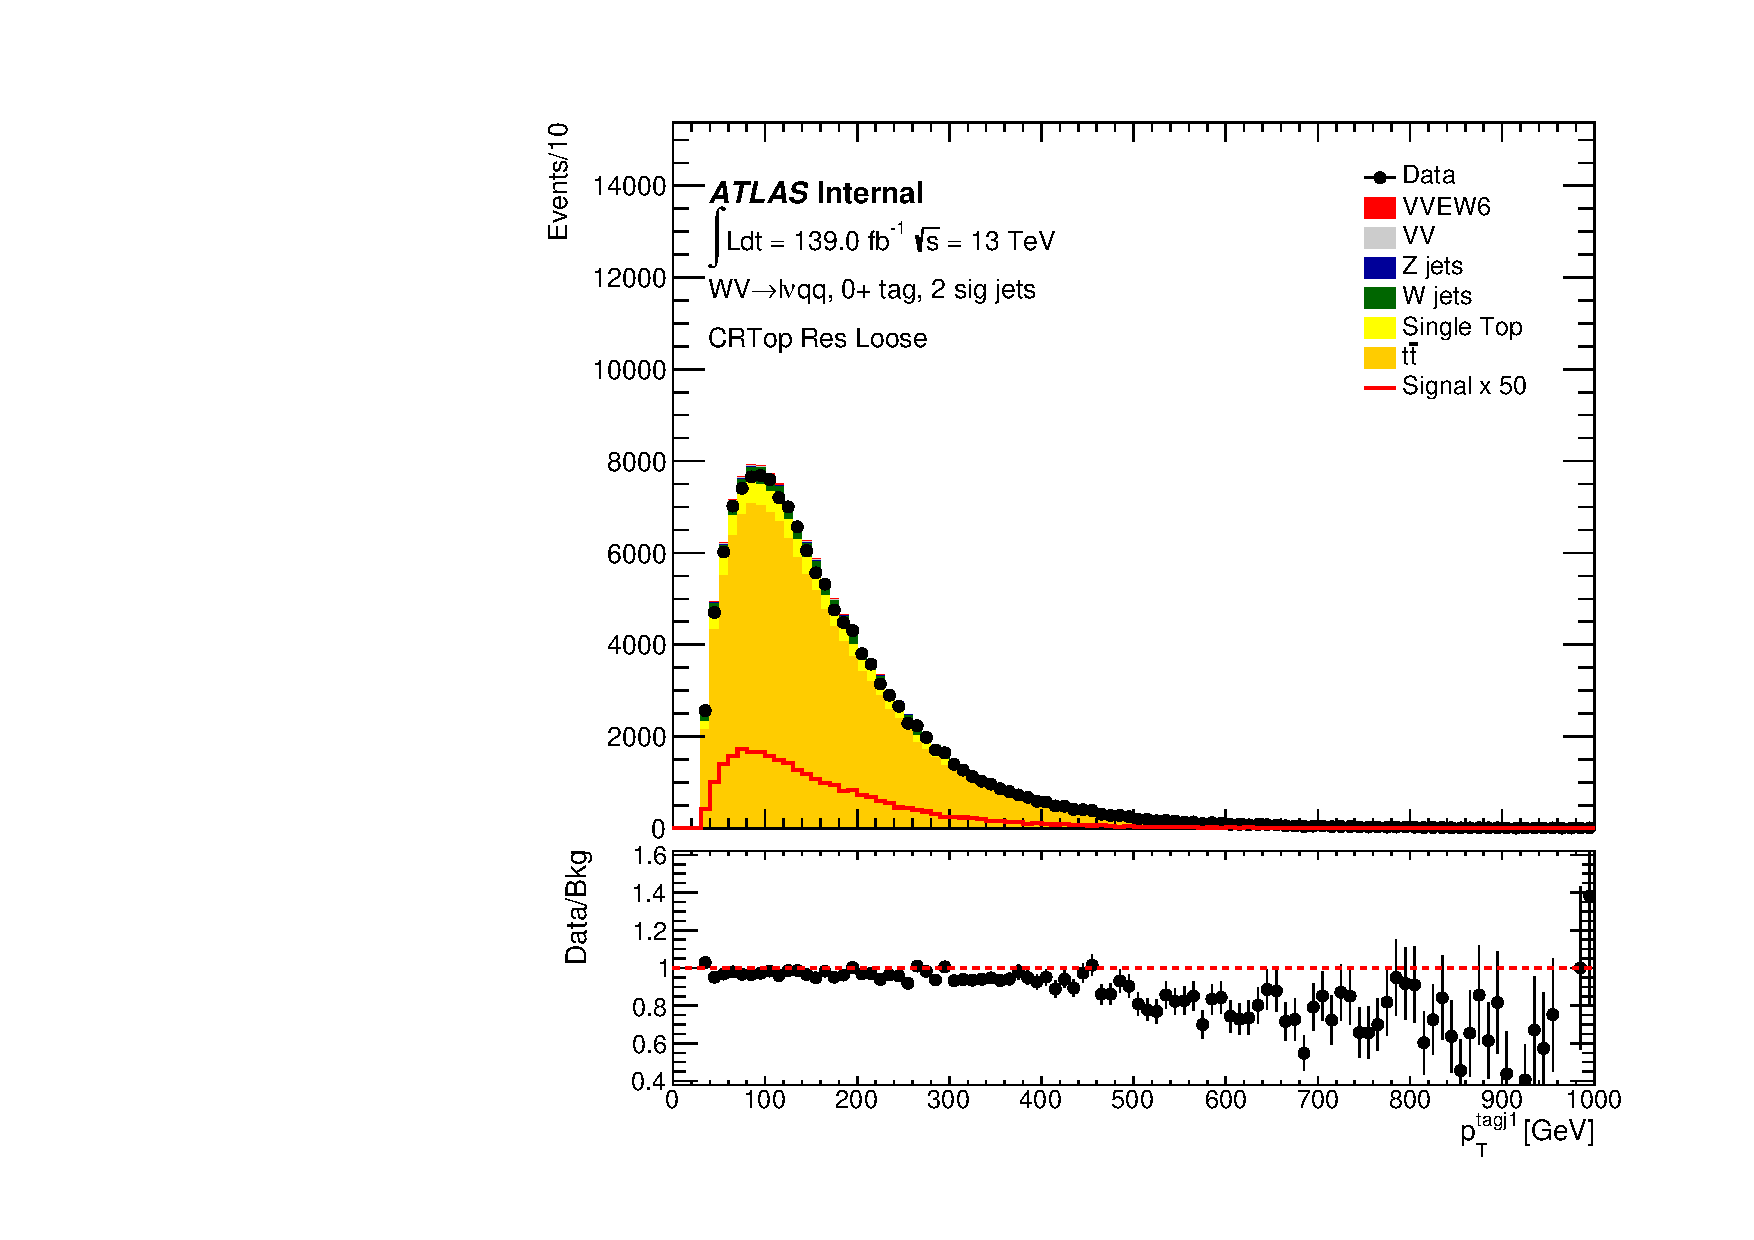
\includegraphics[width=0.3\textwidth]{figures/CRPlots/CRTop_Res_Loose/stacked_plot_resolved_tagJ1_pt.pdf}}
    \subfloat[]{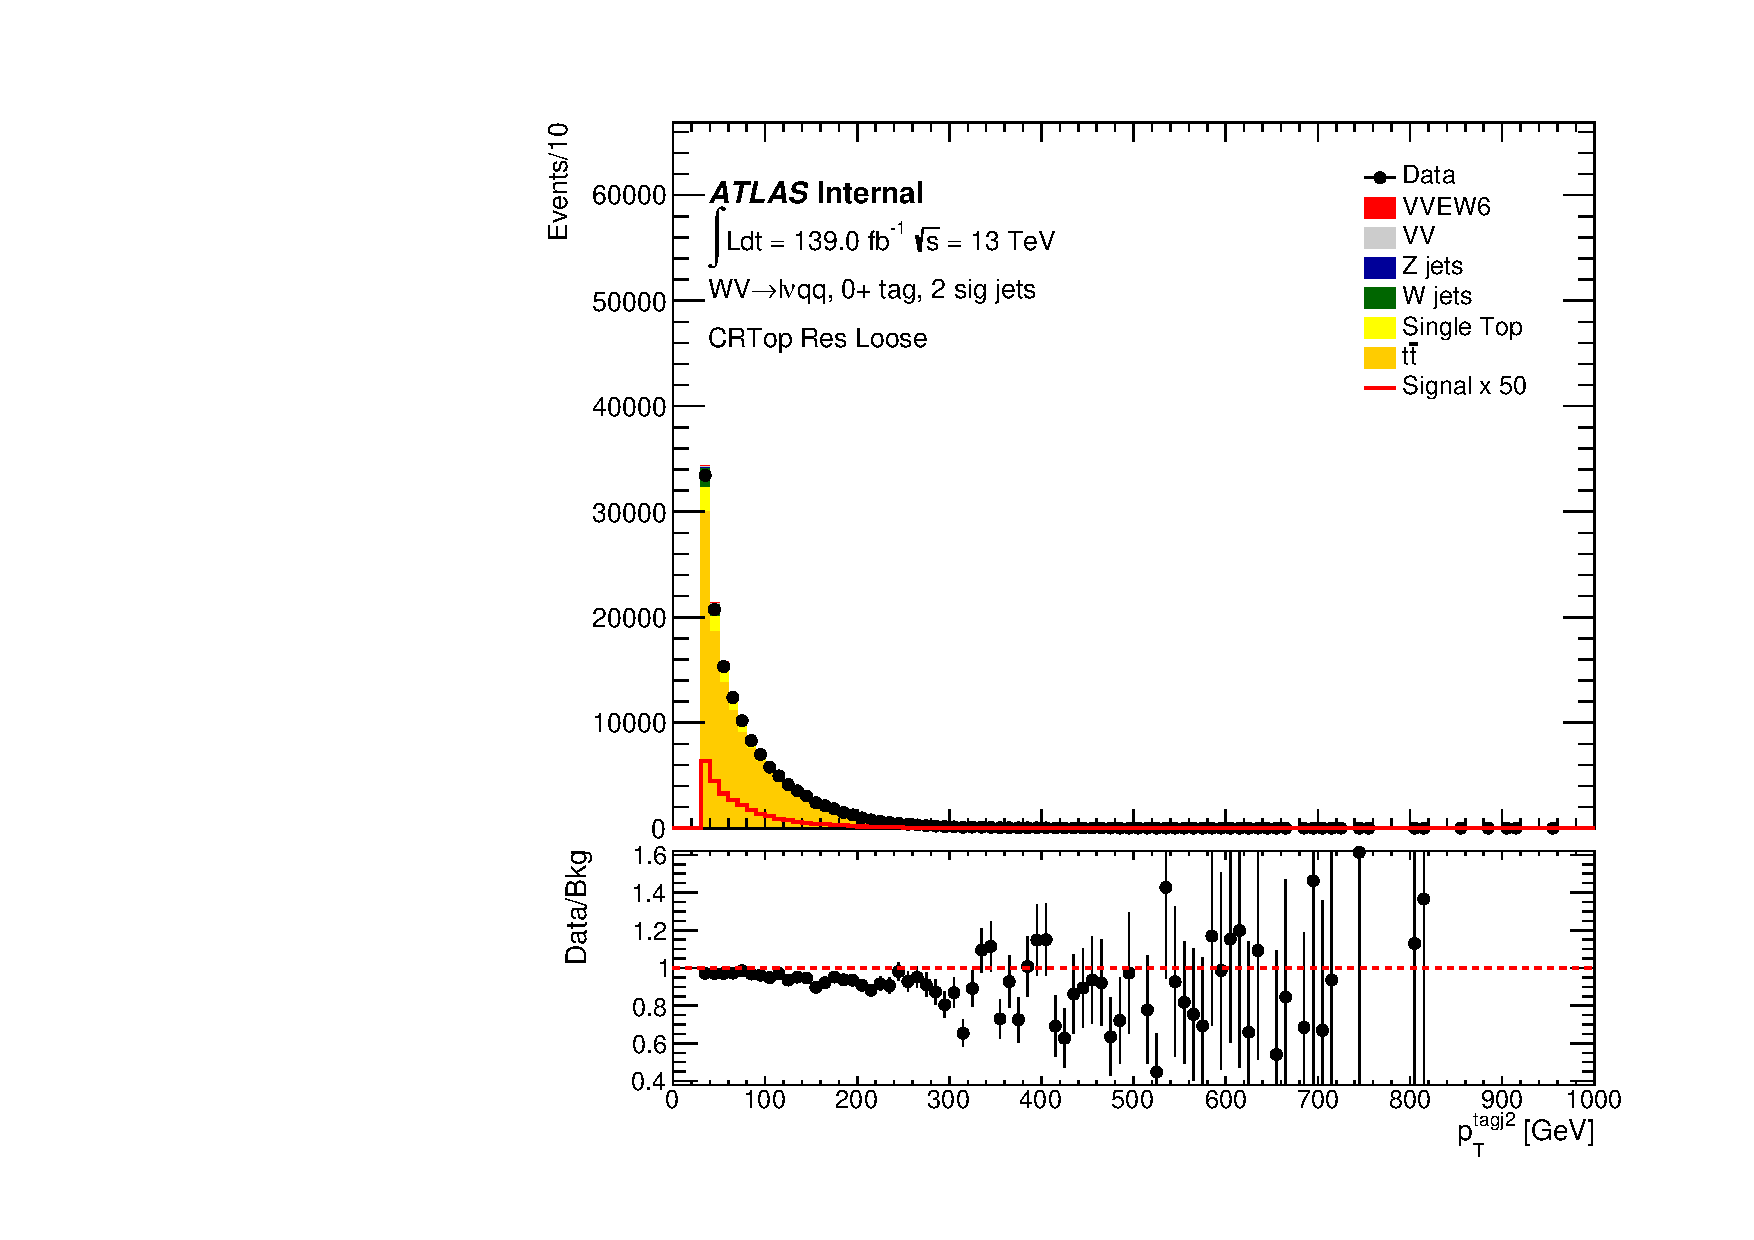
\includegraphics[width=0.3\textwidth]{figures/CRPlots/CRTop_Res_Loose/stacked_plot_resolved_tagJ2_pt.pdf}} \\
    \subfloat[]{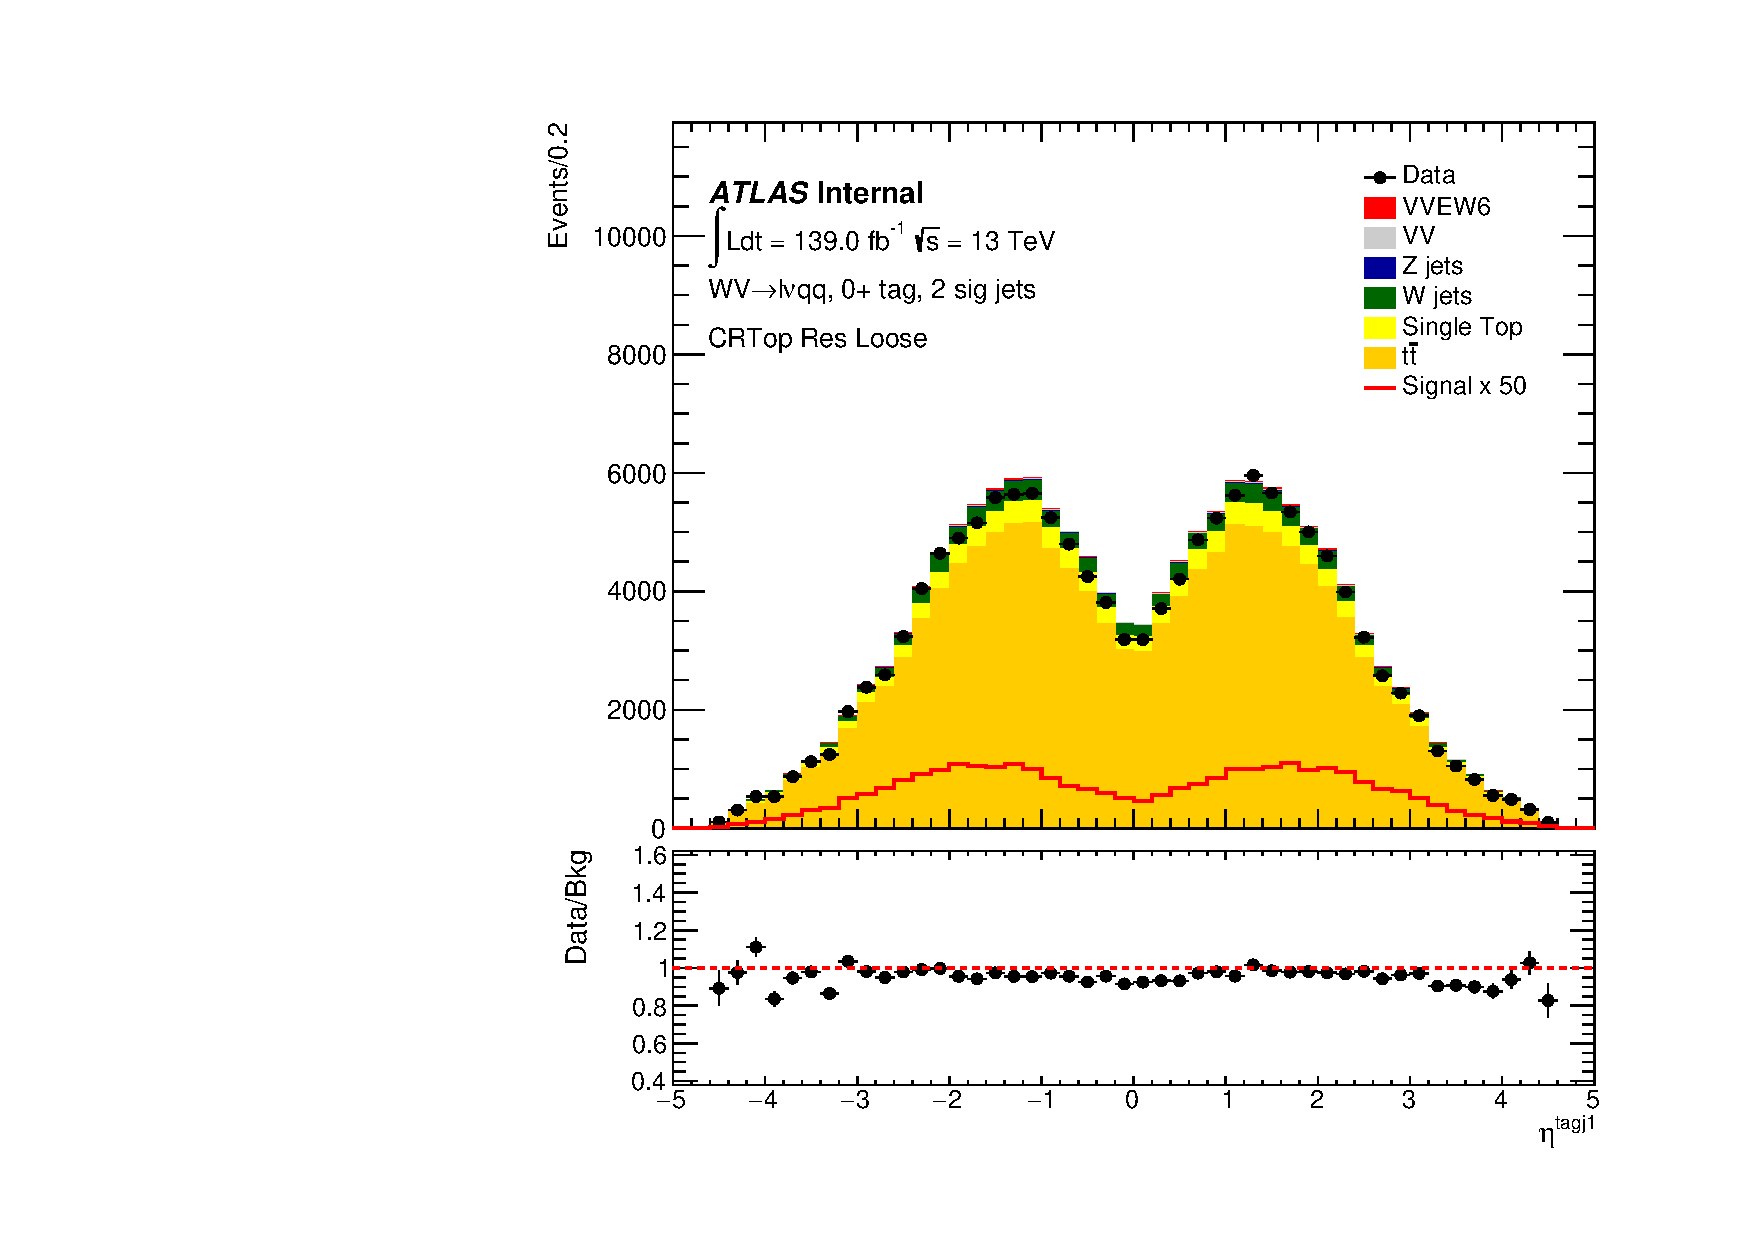
\includegraphics[width=0.3\textwidth]{figures/CRPlots/CRTop_Res_Loose/stacked_plot_resolved_tagJ1_eta.pdf}}
    \subfloat[]{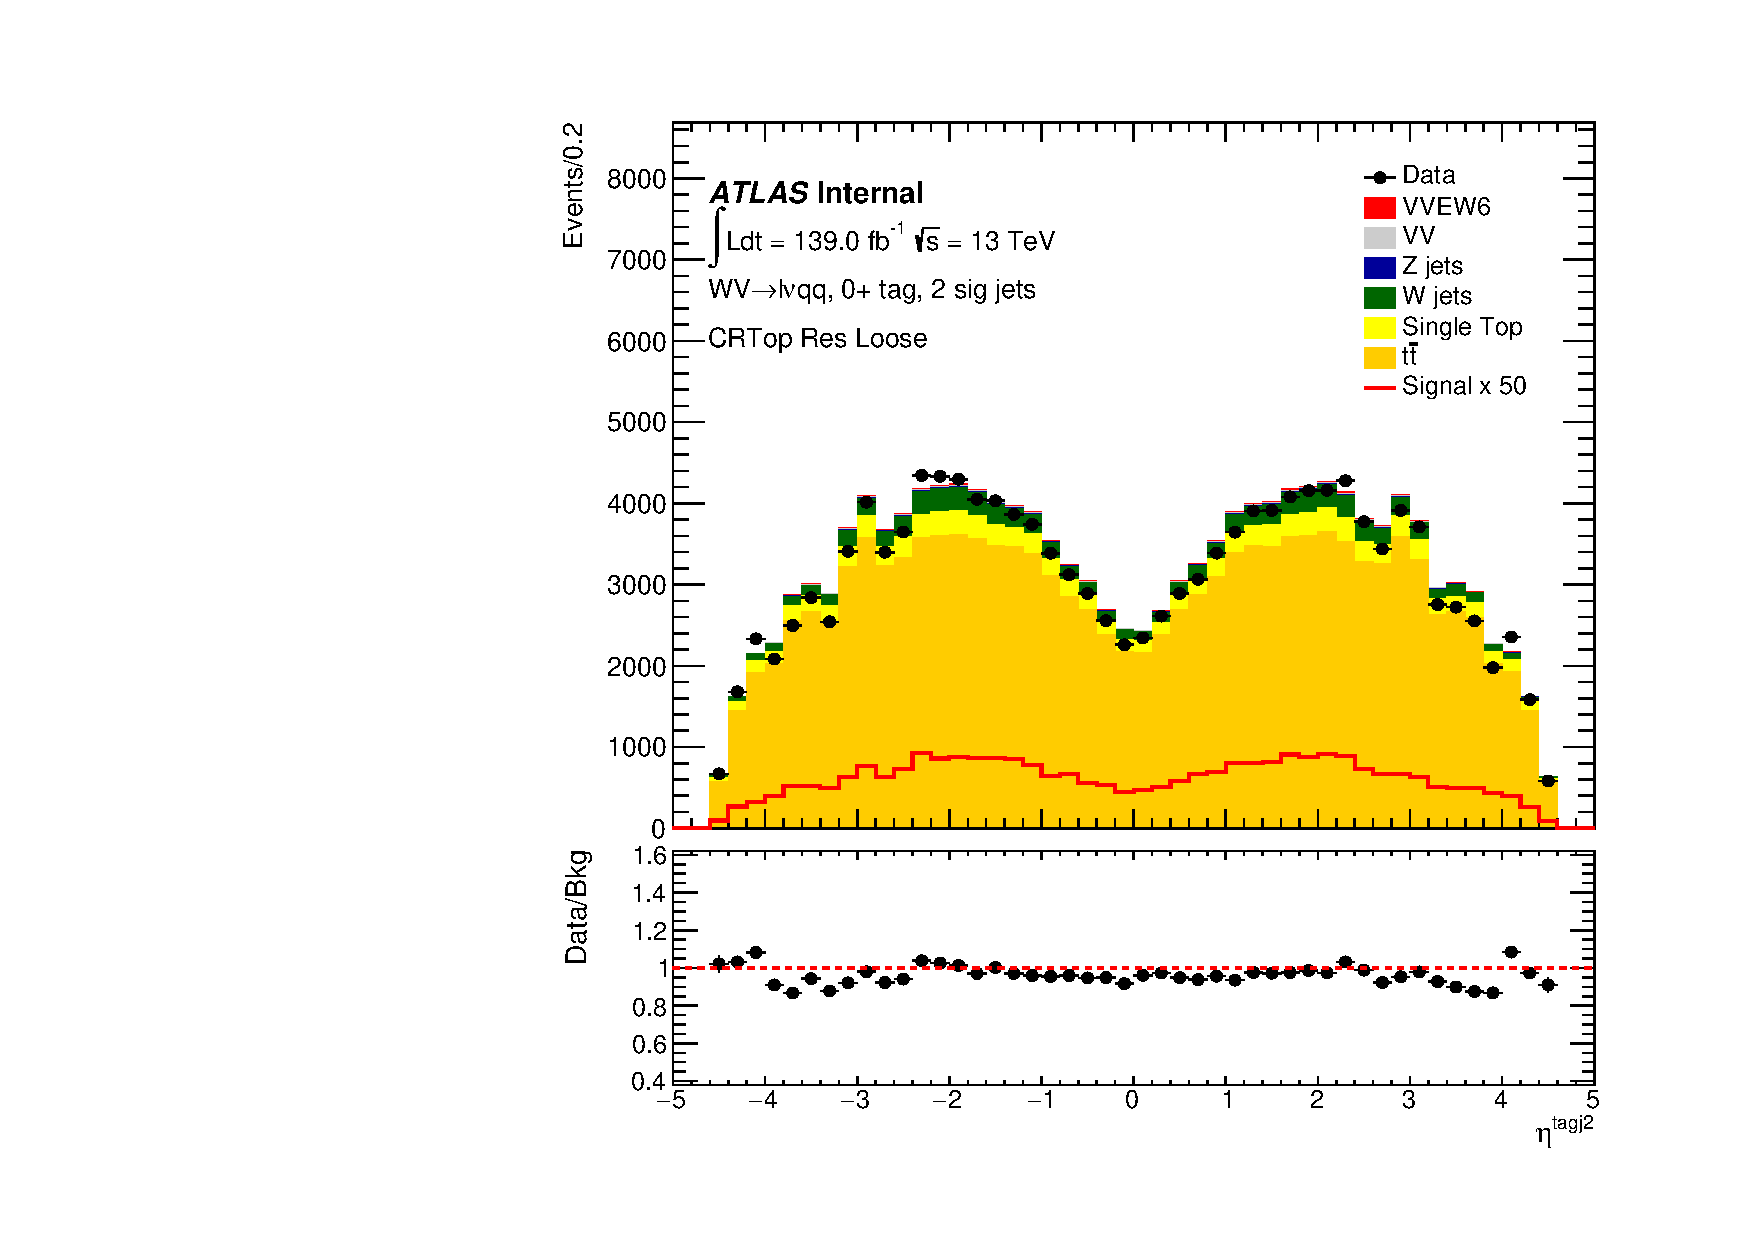
\includegraphics[width=0.3\textwidth]{figures/CRPlots/CRTop_Res_Loose/stacked_plot_resolved_tagJ2_eta.pdf}} \\
    \subfloat[]{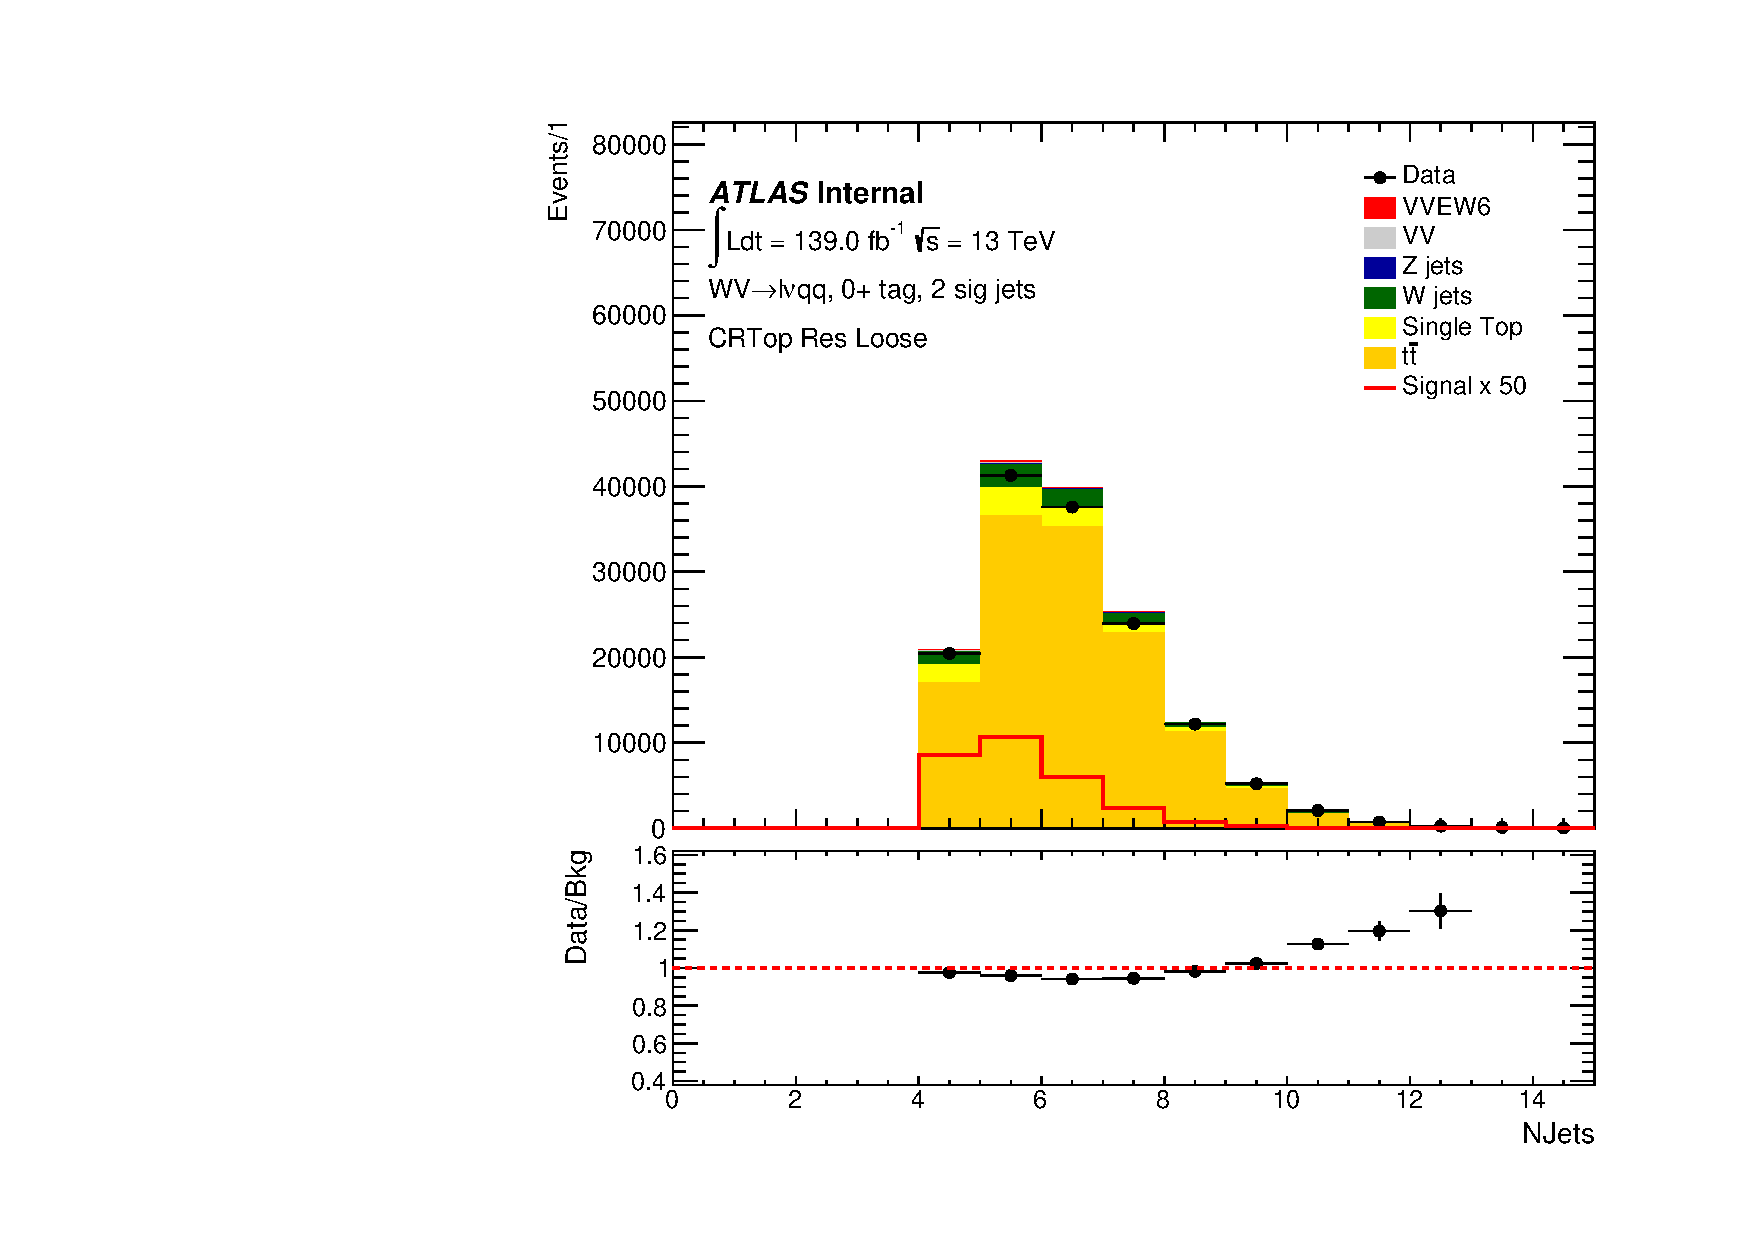
\includegraphics[width=0.3\textwidth]{figures/CRPlots/CRTop_Res_Loose/stacked_plot_NJets.pdf}}
    \subfloat[]{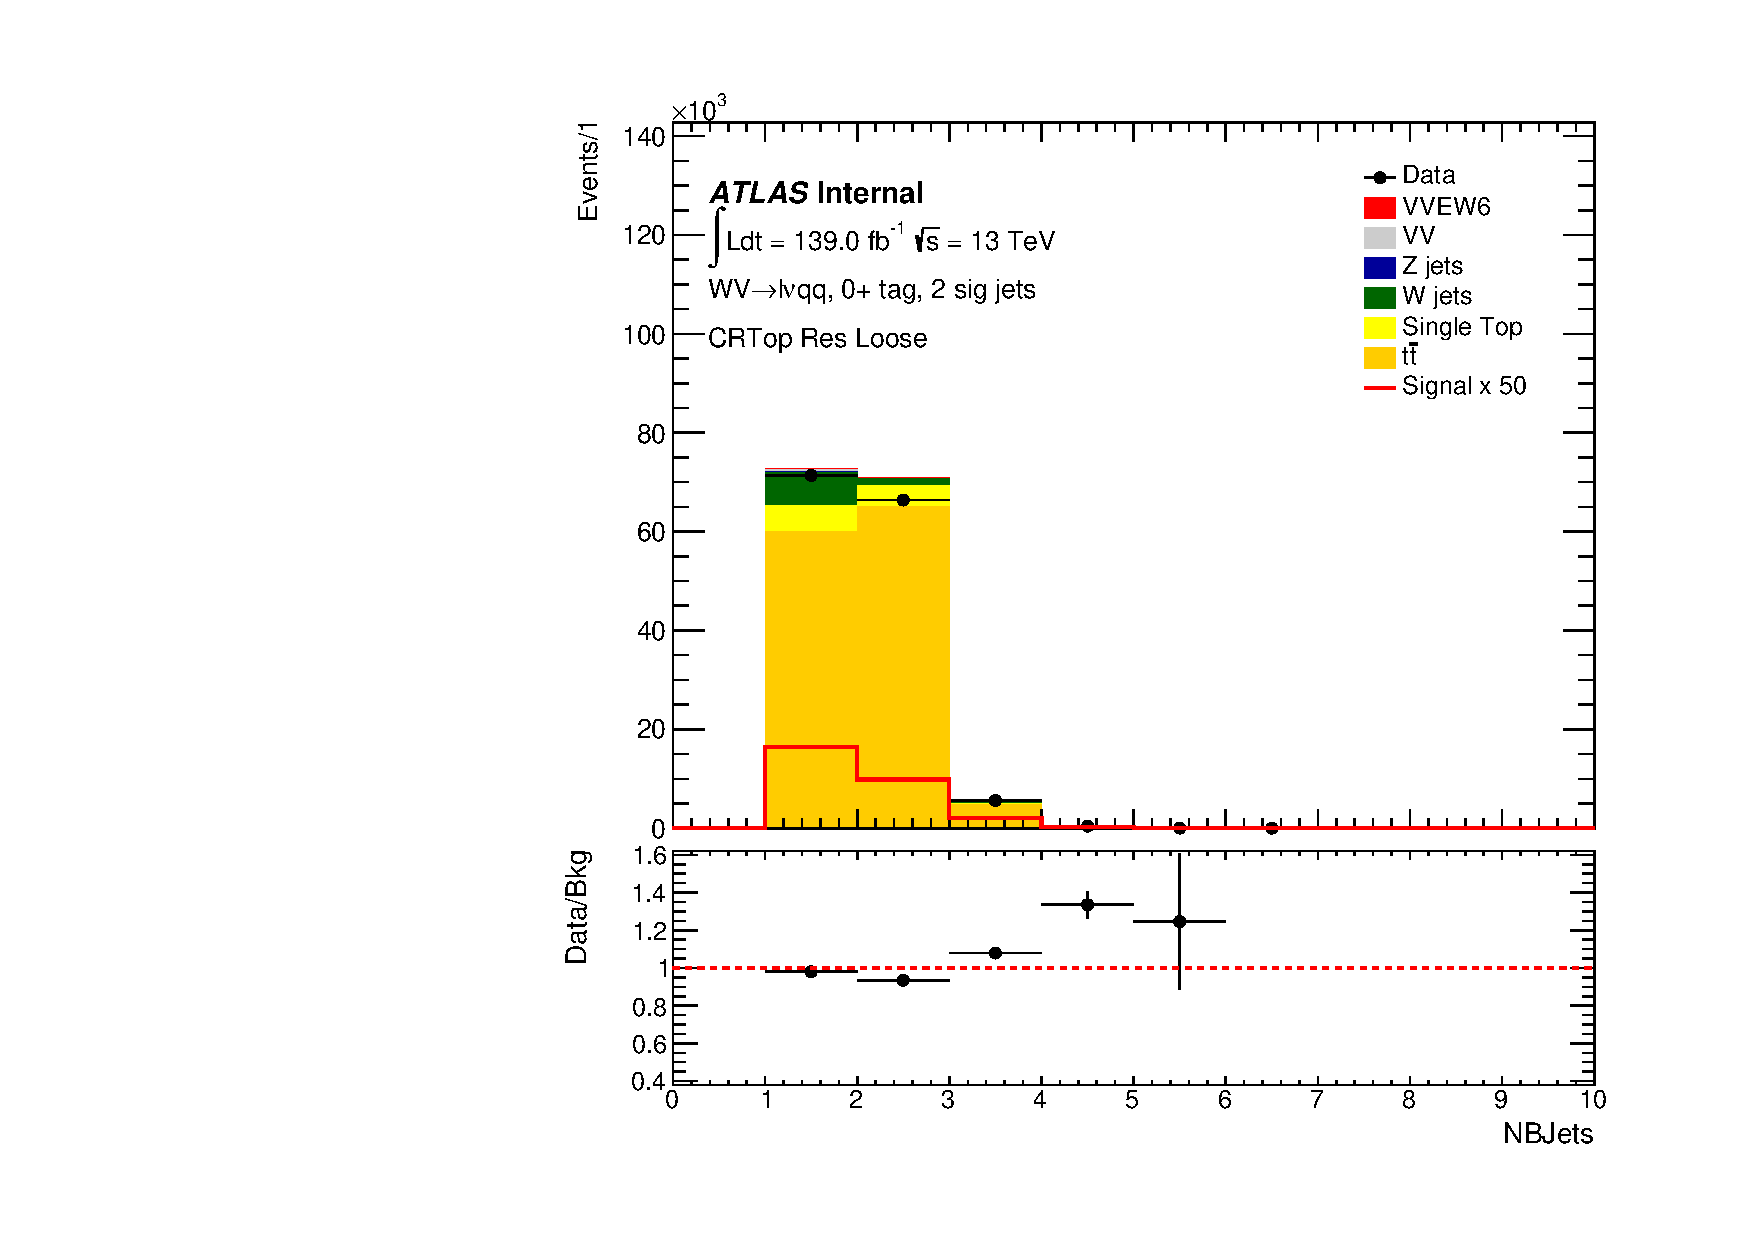
\includegraphics[width=0.3\textwidth]{figures/CRPlots/CRTop_Res_Loose/stacked_plot_NBJets.pdf}}
    \subfloat[]{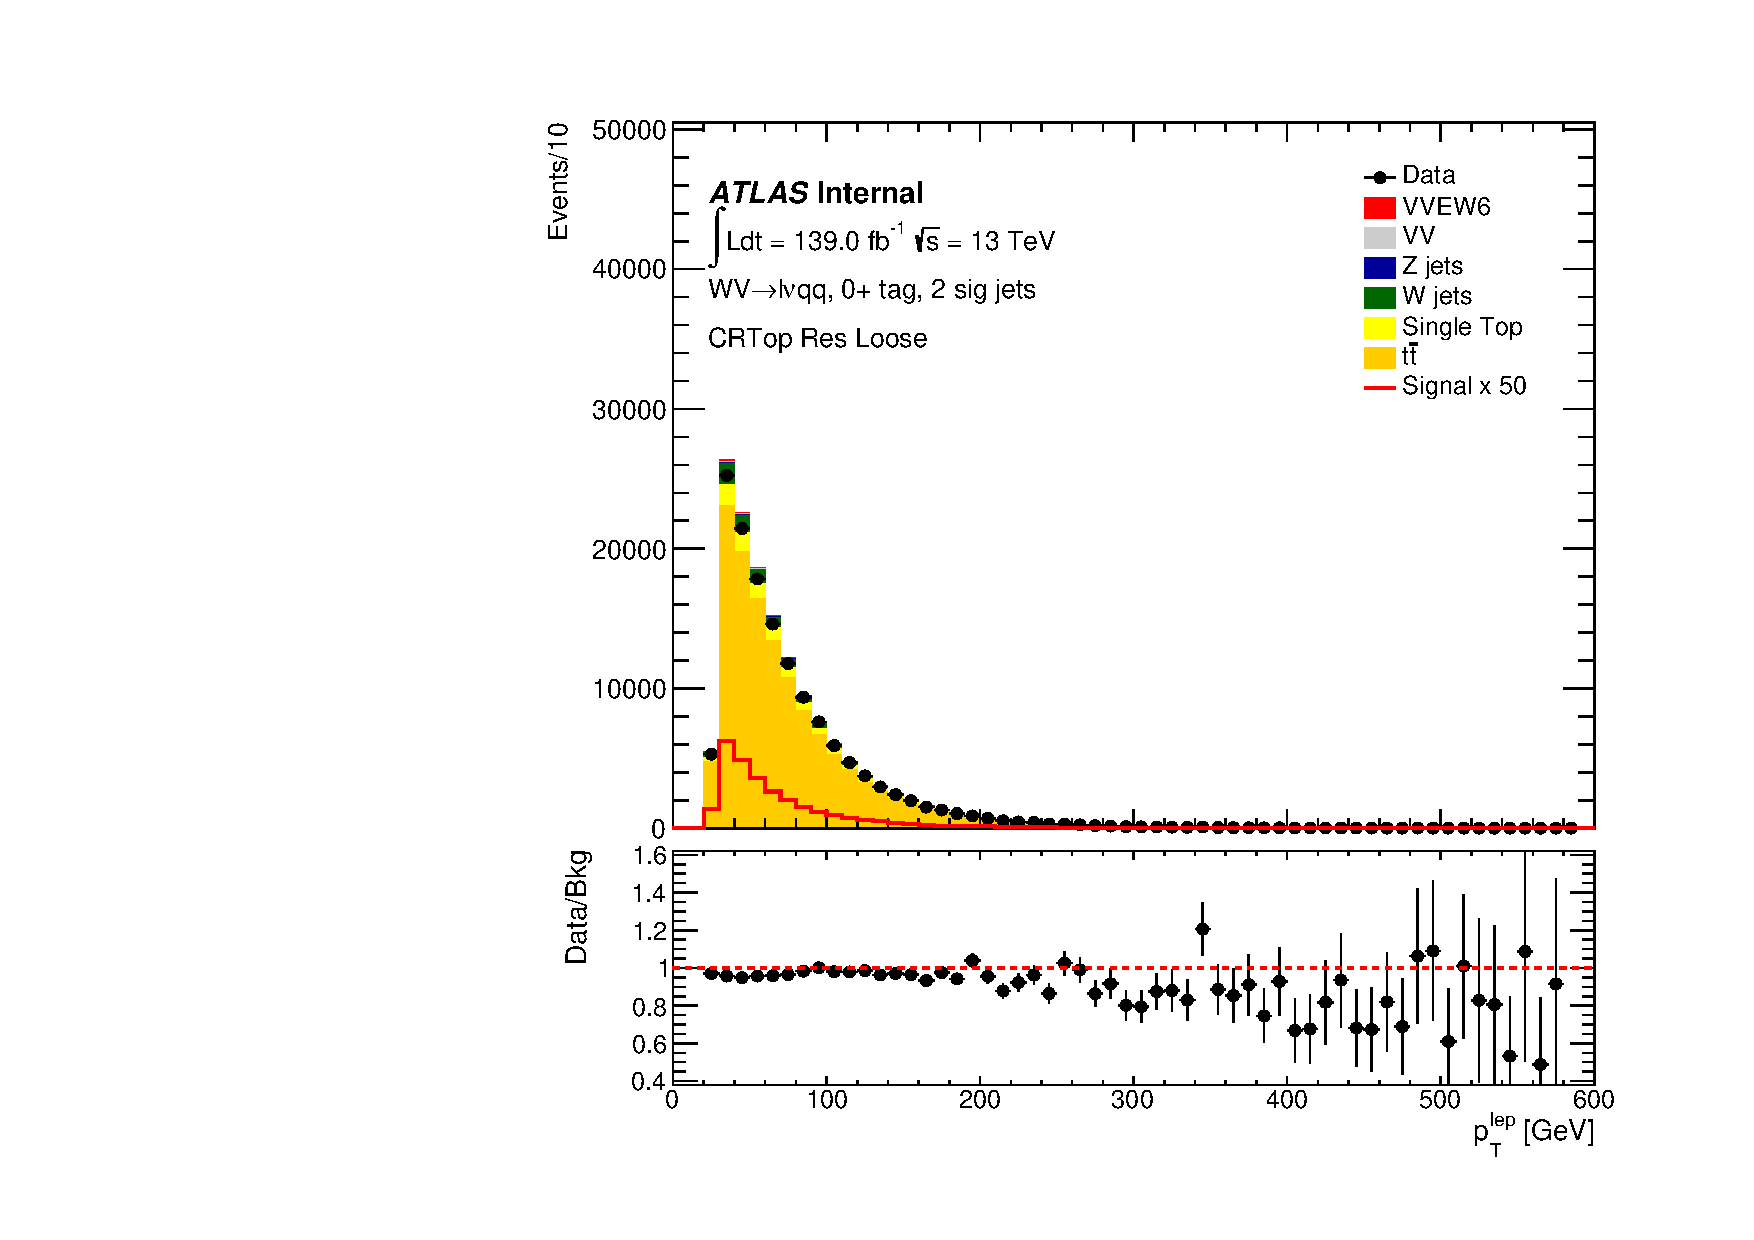
\includegraphics[width=0.3\textwidth]{figures/CRPlots/CRTop_Res_Loose/stacked_plot_lep_pt.pdf}}
    \caption{Data-MC checks for the resolved loose top control region in the \olep channel.}
    \label{fig:CRTopResLoosePlots1Lep}
\end{figure}

\begin{figure}[ht]
    \centering
    \subfloat[]{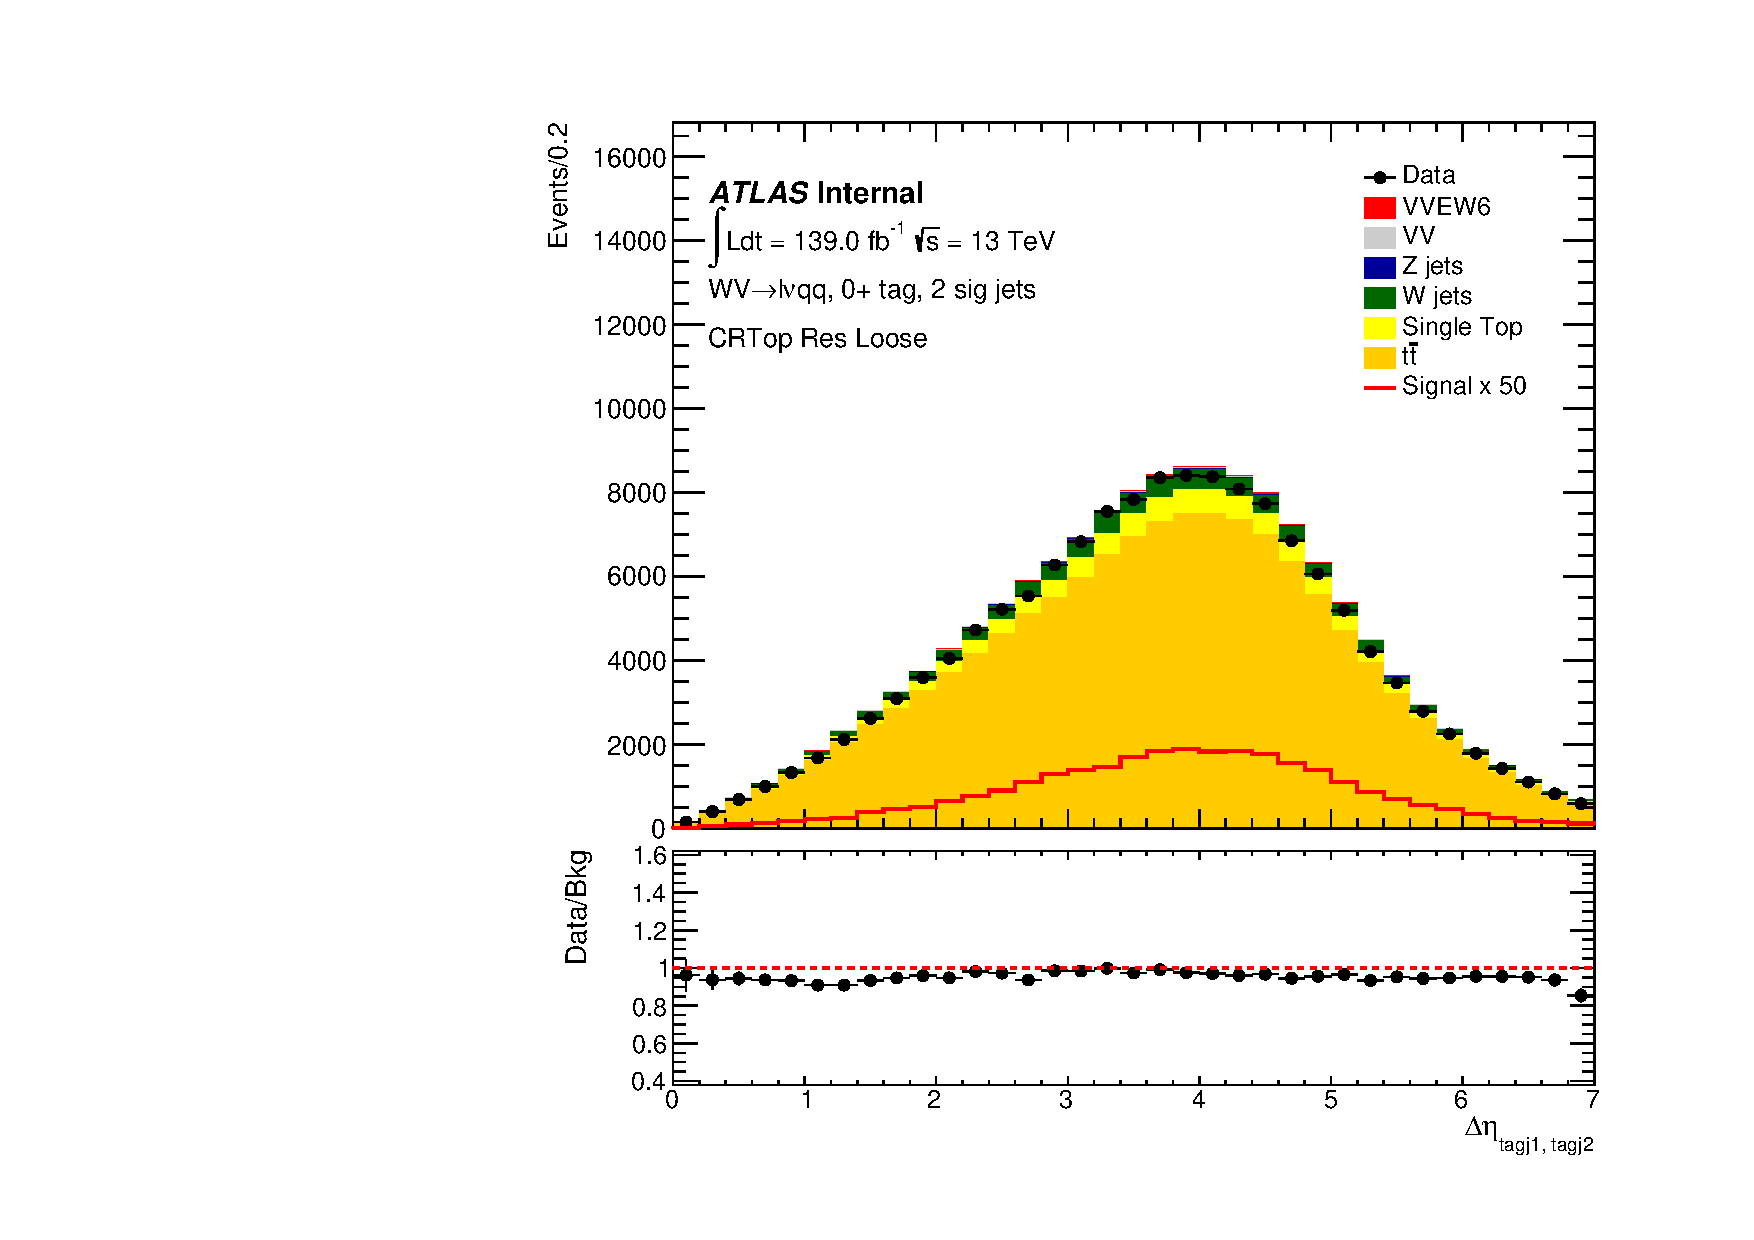
\includegraphics[width=0.3\textwidth]{figures/CRPlots/CRTop_Res_Loose/stacked_plot_resolved_tagJdEta.pdf}}
    \subfloat[]{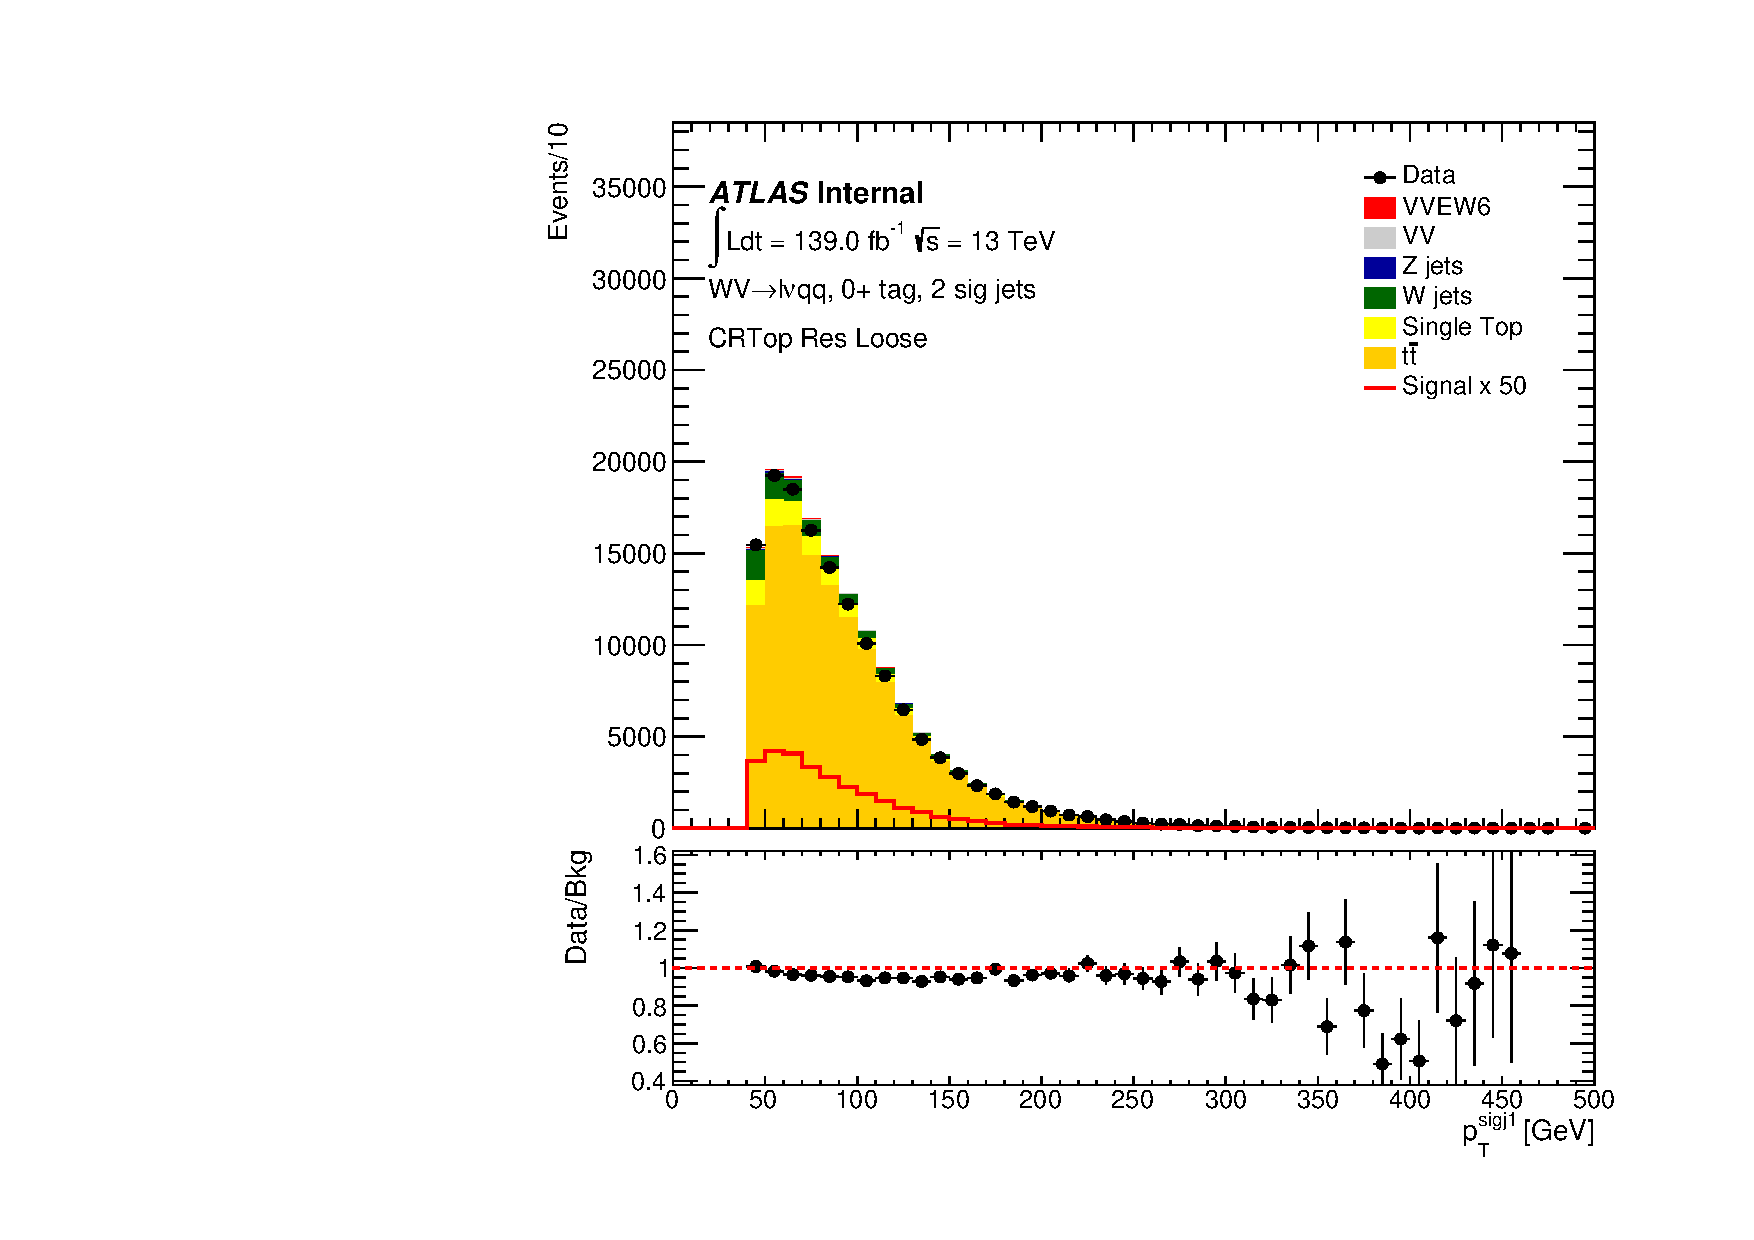
\includegraphics[width=0.3\textwidth]{figures/CRPlots/CRTop_Res_Loose/stacked_plot_sigJ1_pt.pdf}}
    \subfloat[]{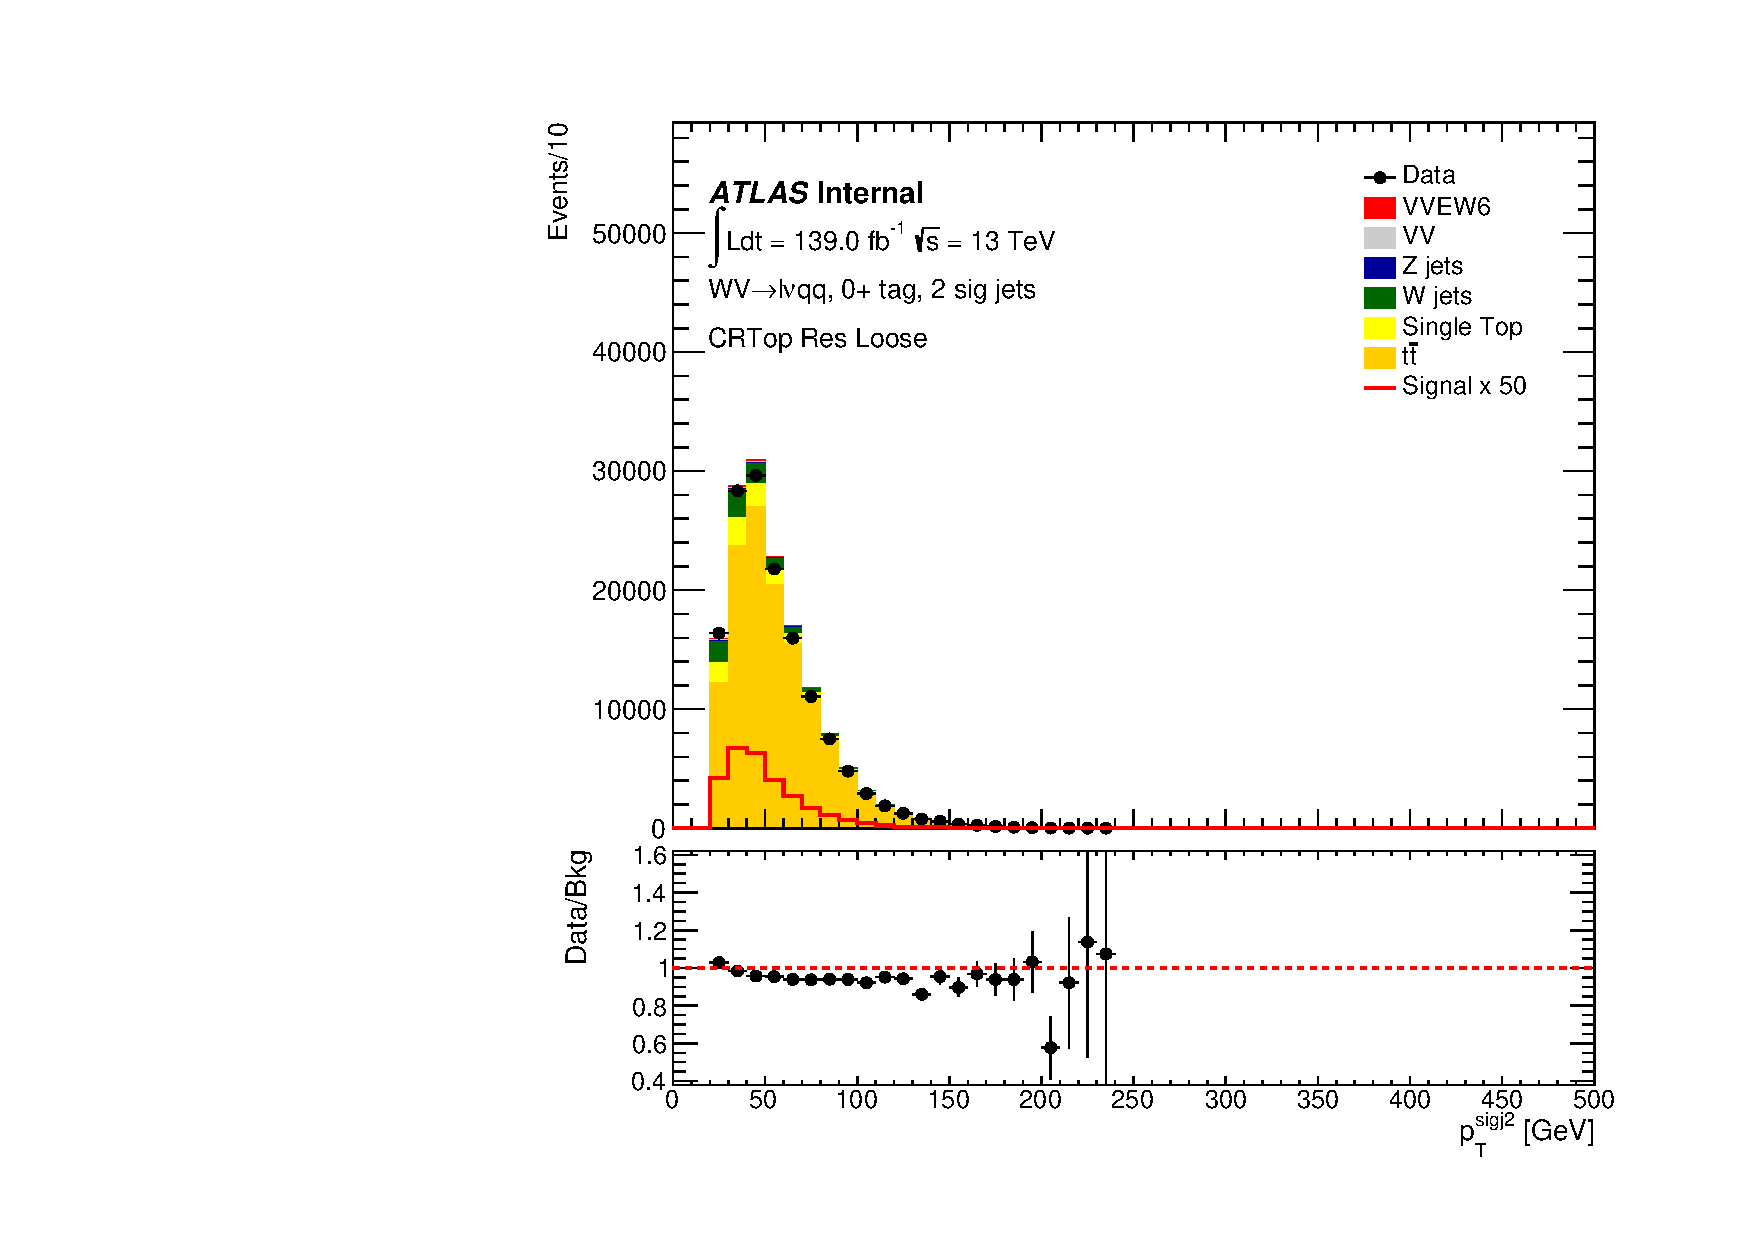
\includegraphics[width=0.3\textwidth]{figures/CRPlots/CRTop_Res_Loose/stacked_plot_sigJ2_pt.pdf}} \\
    \subfloat[]{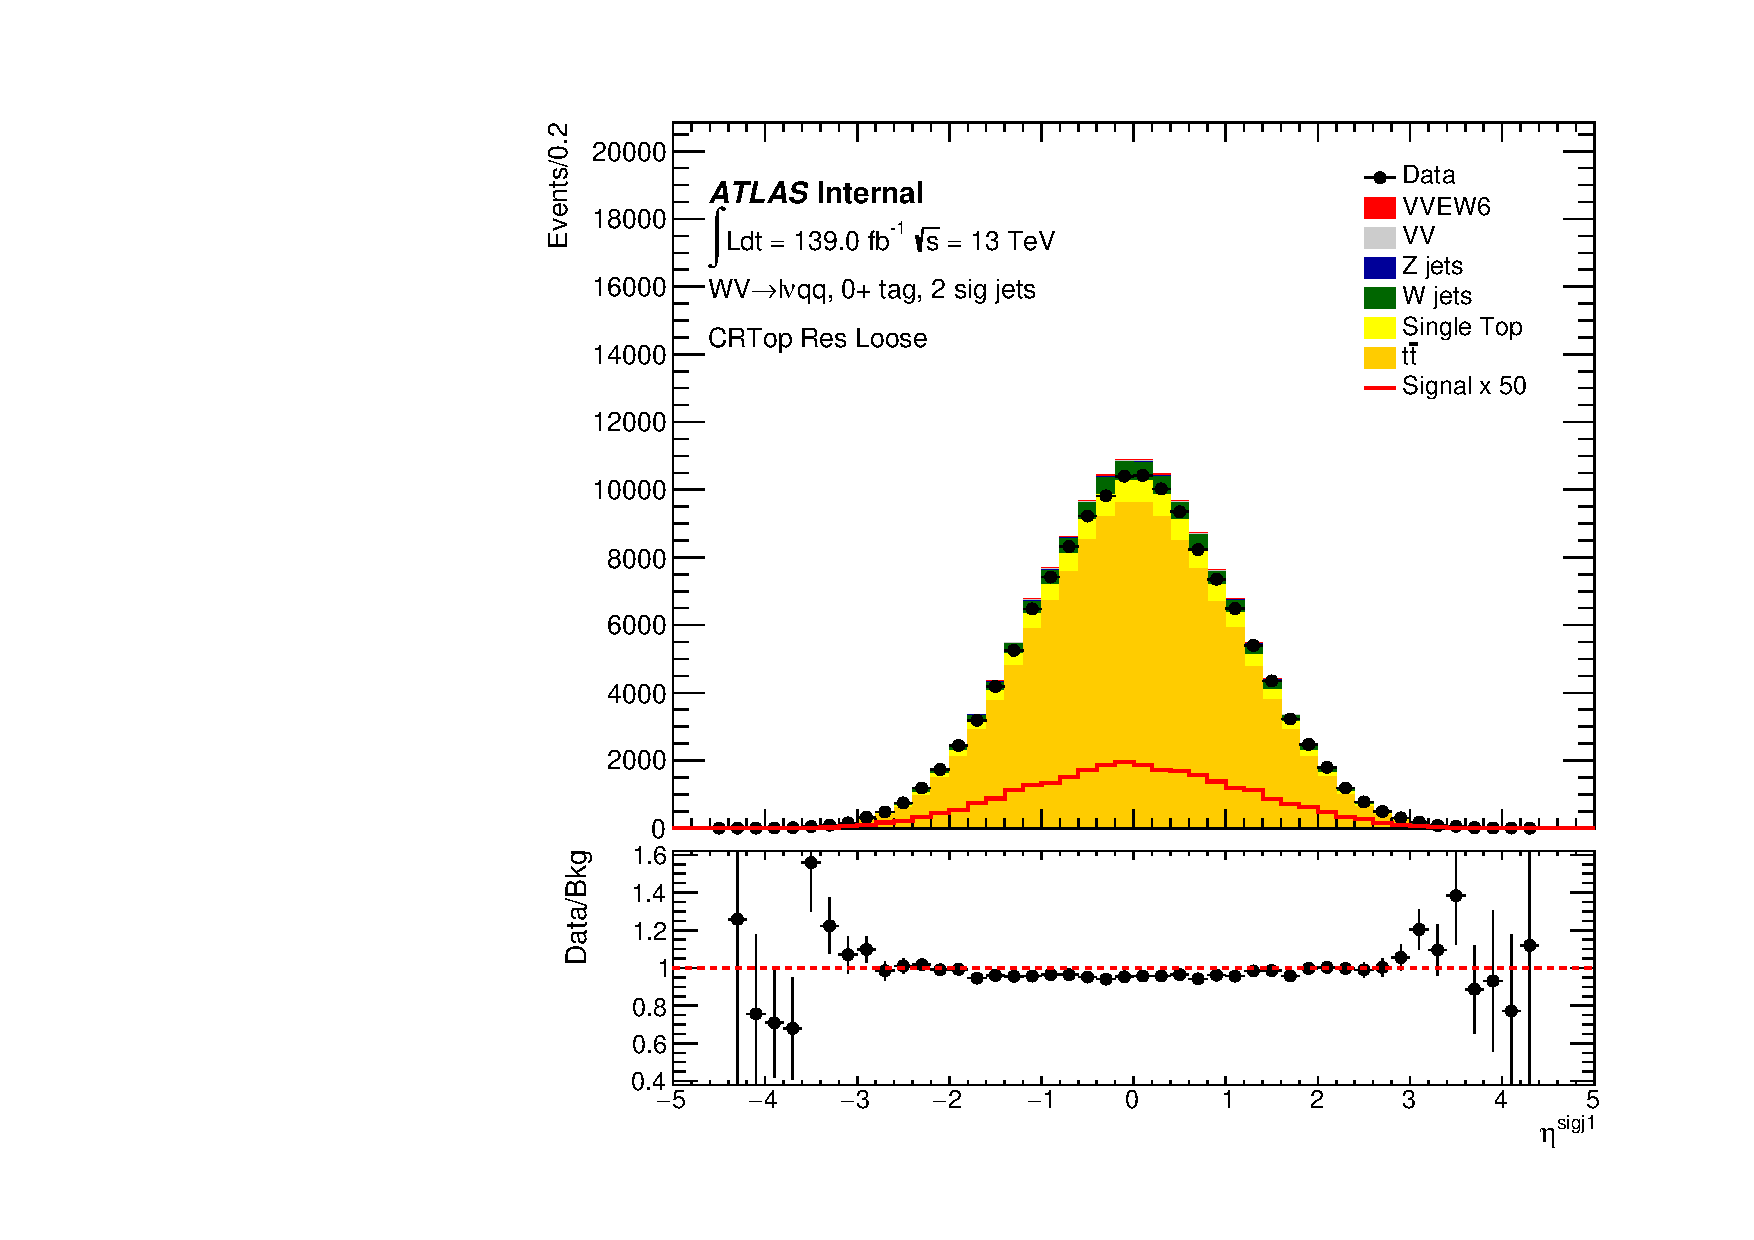
\includegraphics[width=0.3\textwidth]{figures/CRPlots/CRTop_Res_Loose/stacked_plot_sigJ1_eta.pdf}}
    \subfloat[]{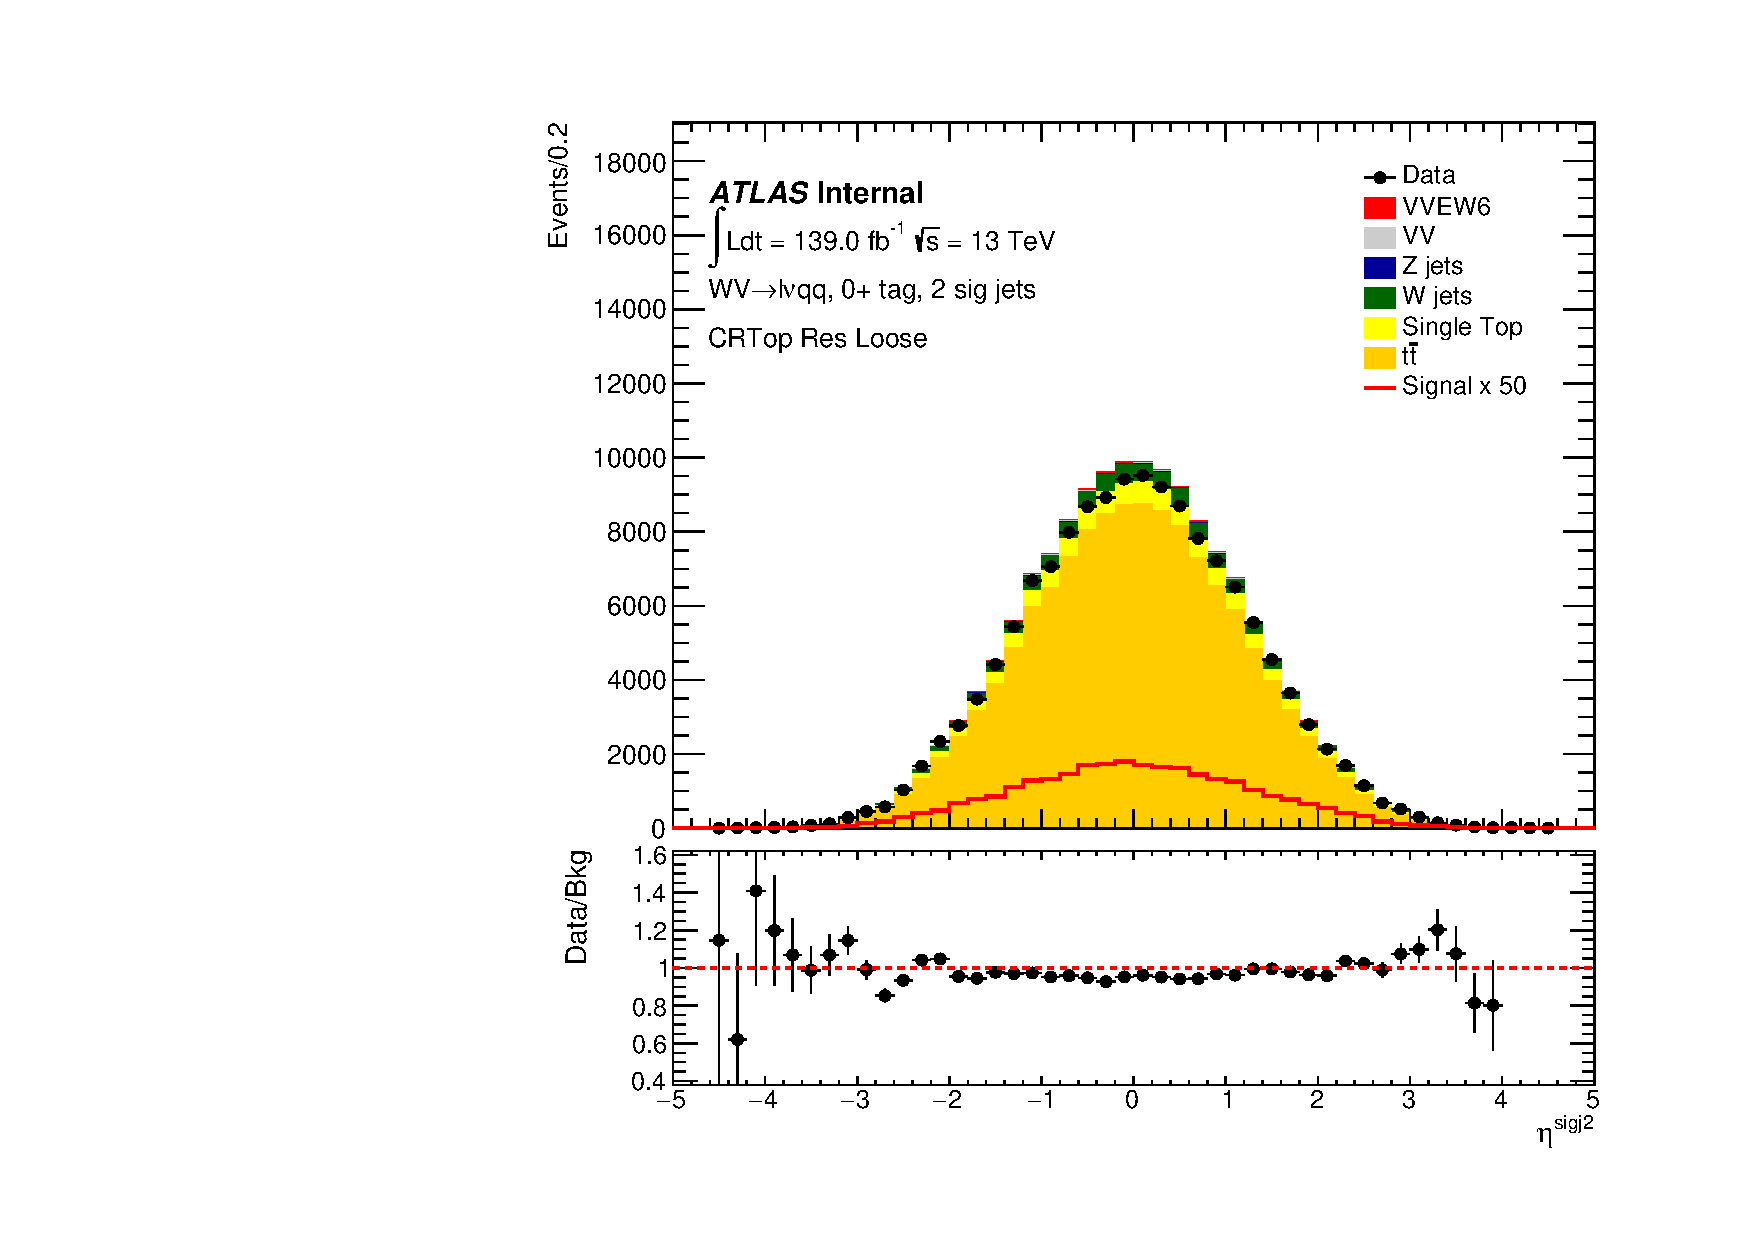
\includegraphics[width=0.3\textwidth]{figures/CRPlots/CRTop_Res_Loose/stacked_plot_sigJ2_eta.pdf}} \\
    \subfloat[]{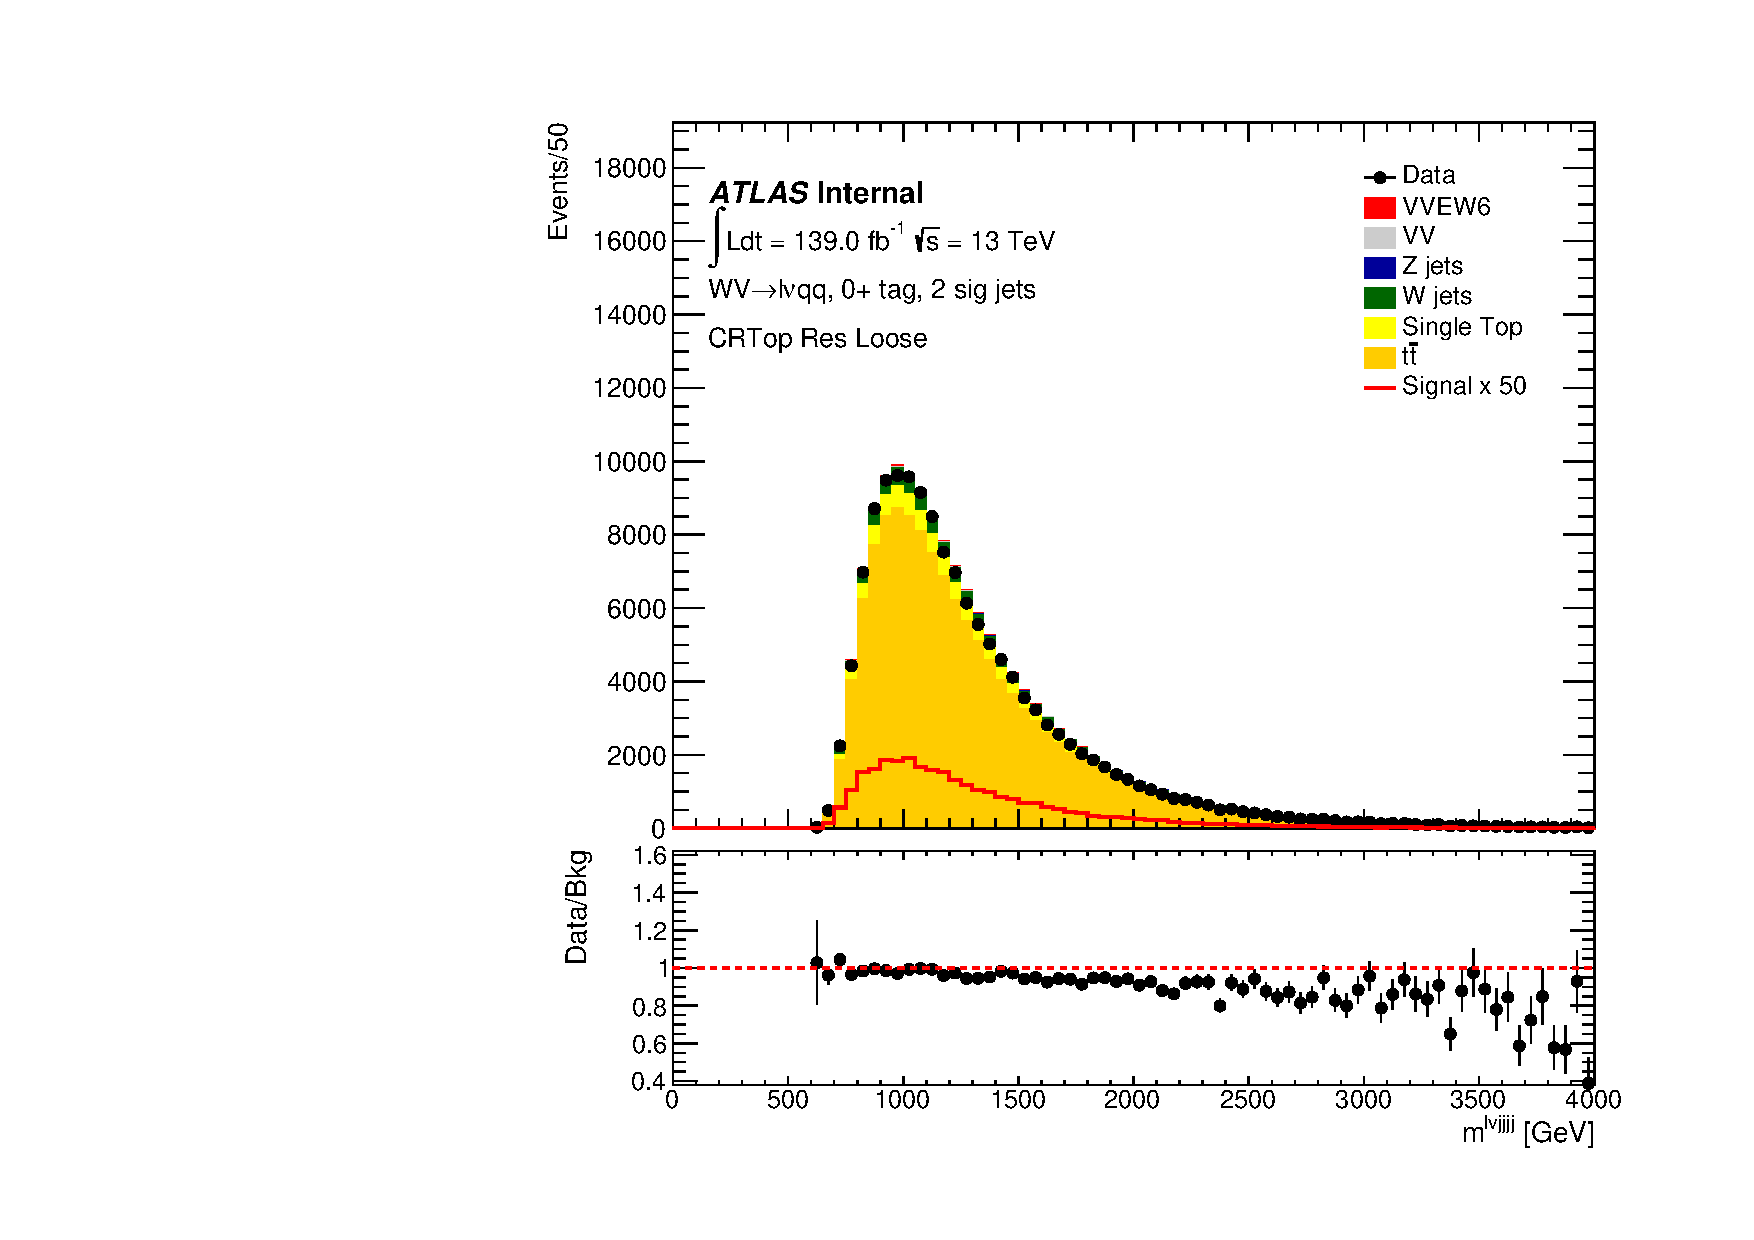
\includegraphics[width=0.3\textwidth]{figures/CRPlots/CRTop_Res_Loose/stacked_plot_lvjjjjmass.pdf}}
    \subfloat[]{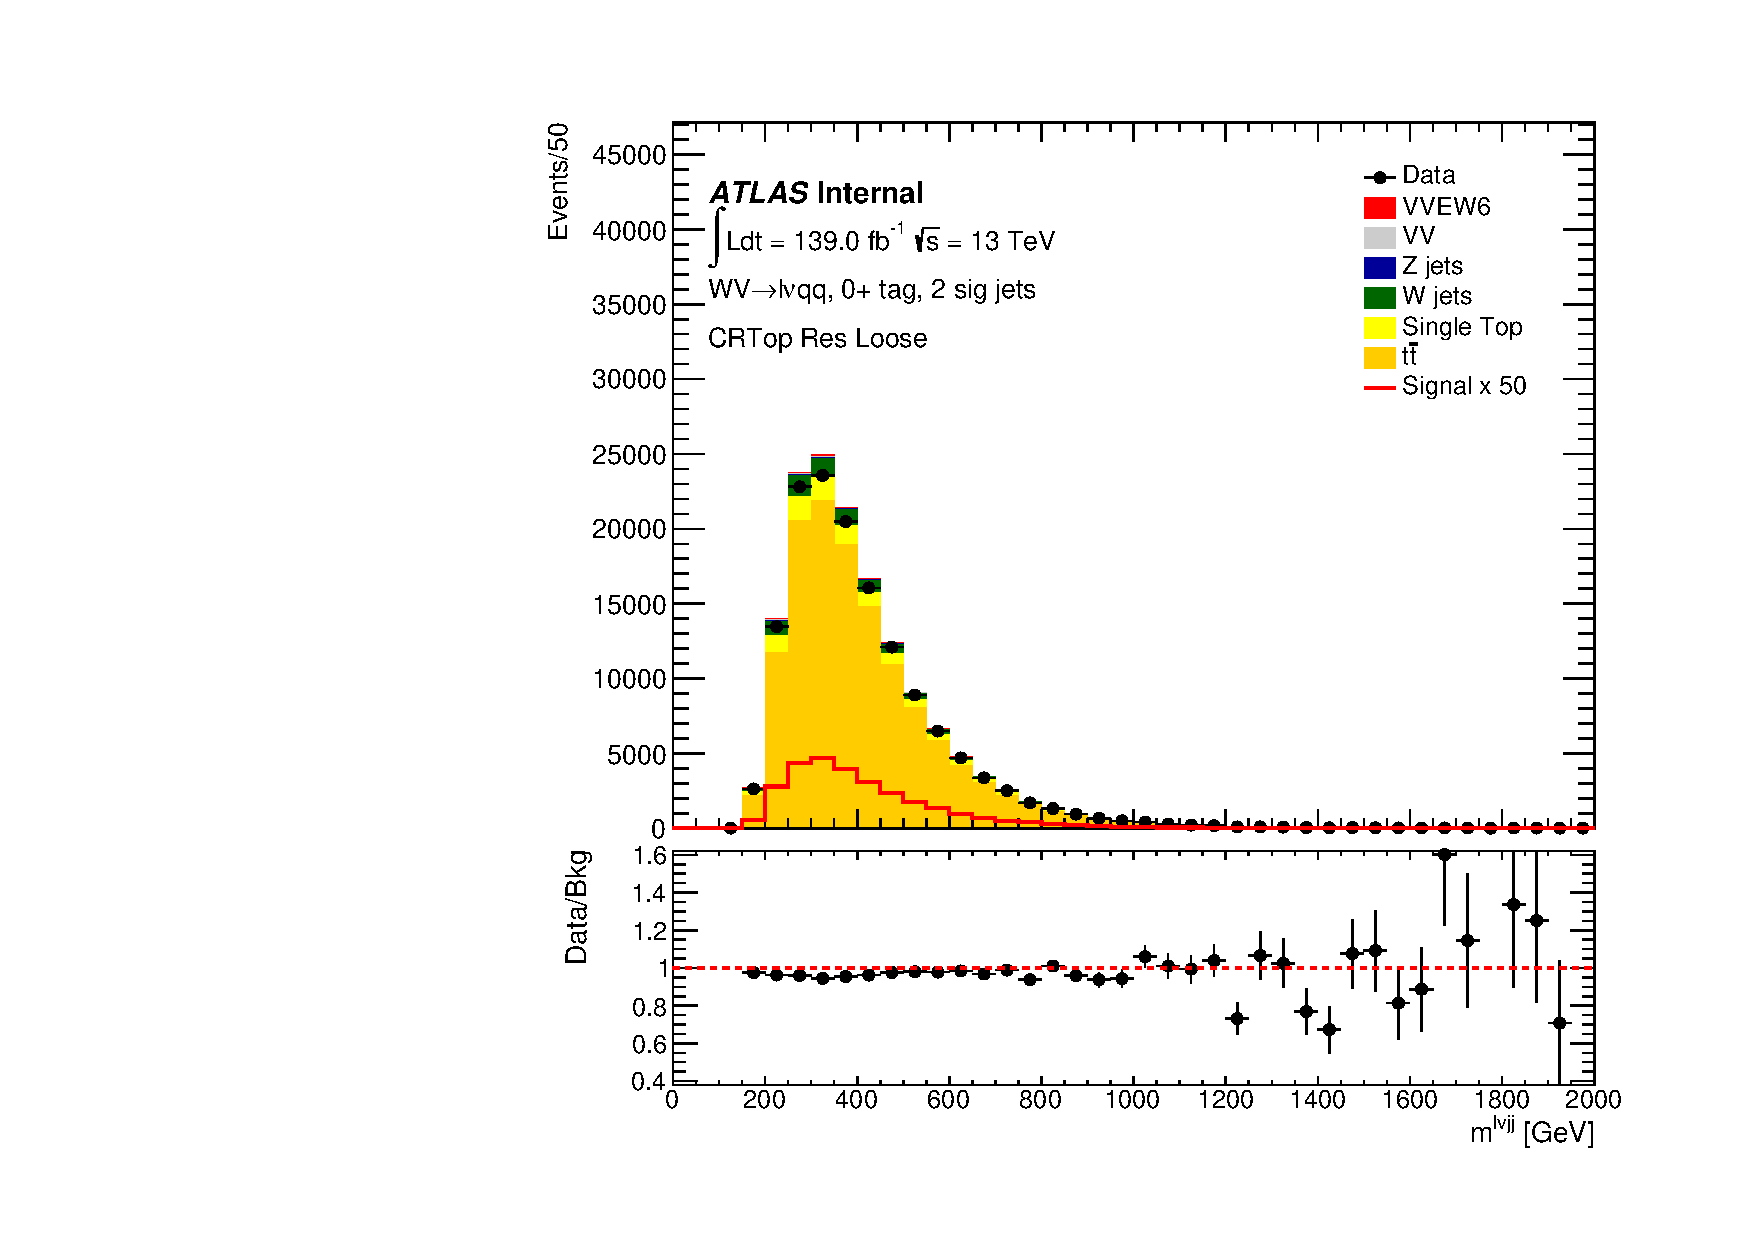
\includegraphics[width=0.3\textwidth]{figures/CRPlots/CRTop_Res_Loose/stacked_plot_lvjjmass.pdf}}
    \subfloat[]{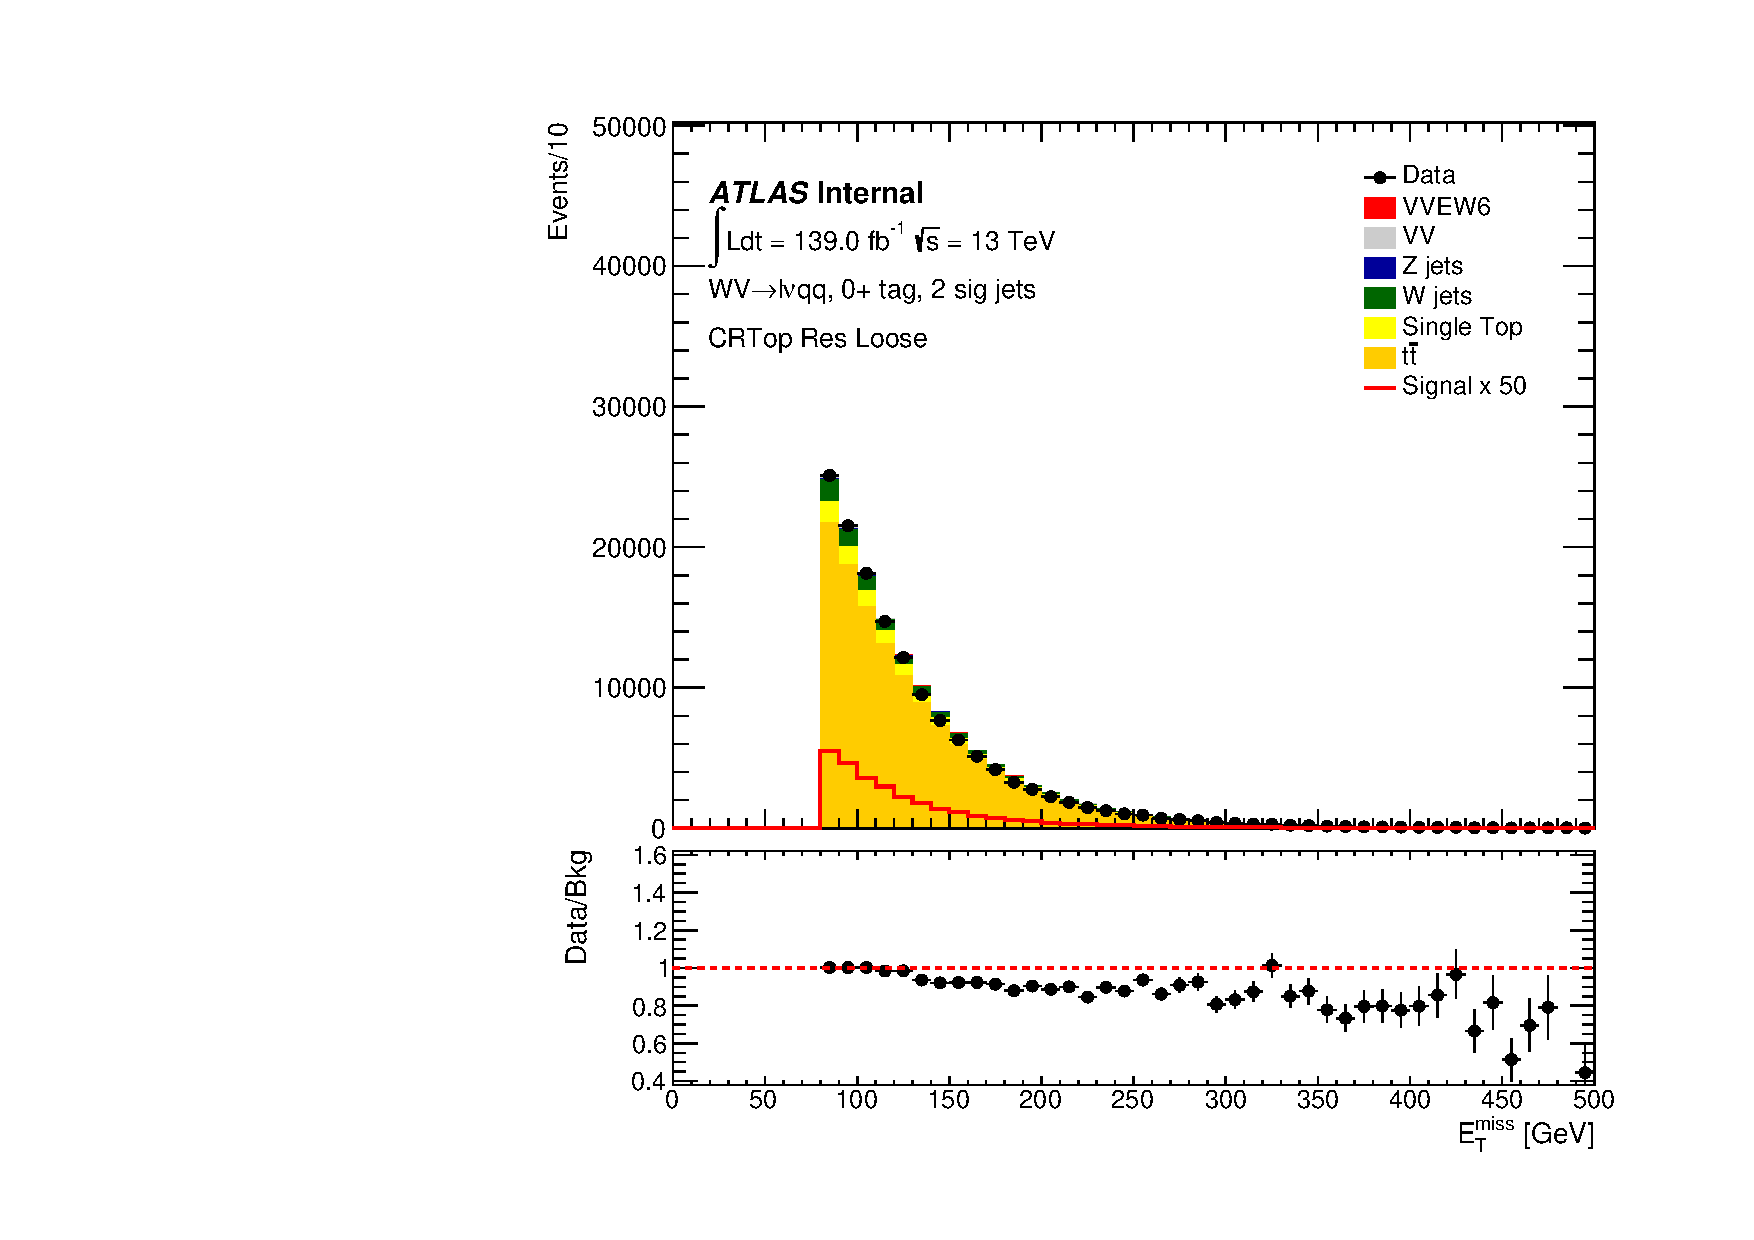
\includegraphics[width=0.3\textwidth]{figures/CRPlots/CRTop_Res_Loose/stacked_plot_met.pdf}}  \\
    \caption{Data-MC checks for the resolved loose top control region in the \olep channel.}
    \label{fig:CRTopResLoosePlots1Lep2}
\end{figure}

\begin{figure}[ht]
    \centering
    \subfloat[]{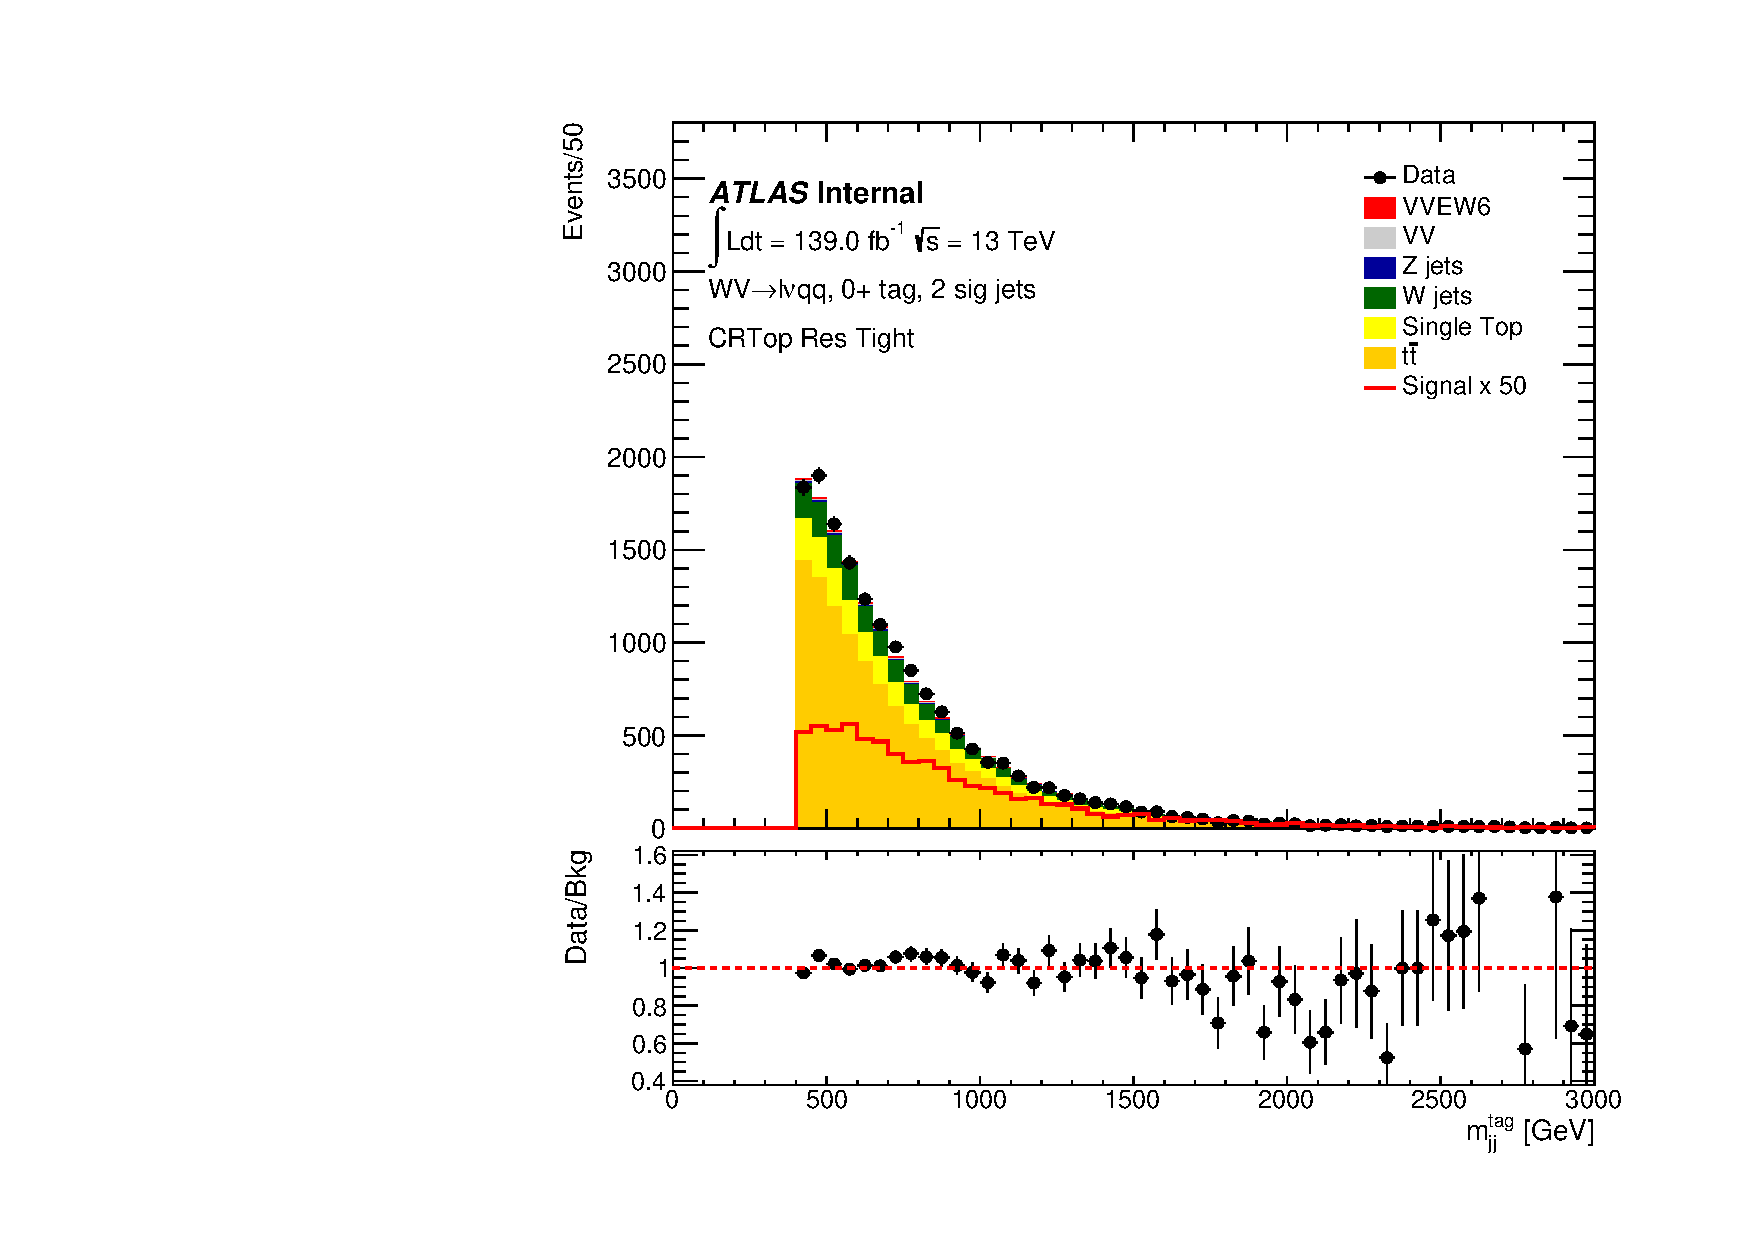
\includegraphics[width=0.3\textwidth]{figures/CRPlots/CRTop_Res_Tight/stacked_plot_resolved_tagMjj.pdf}}
    \subfloat[]{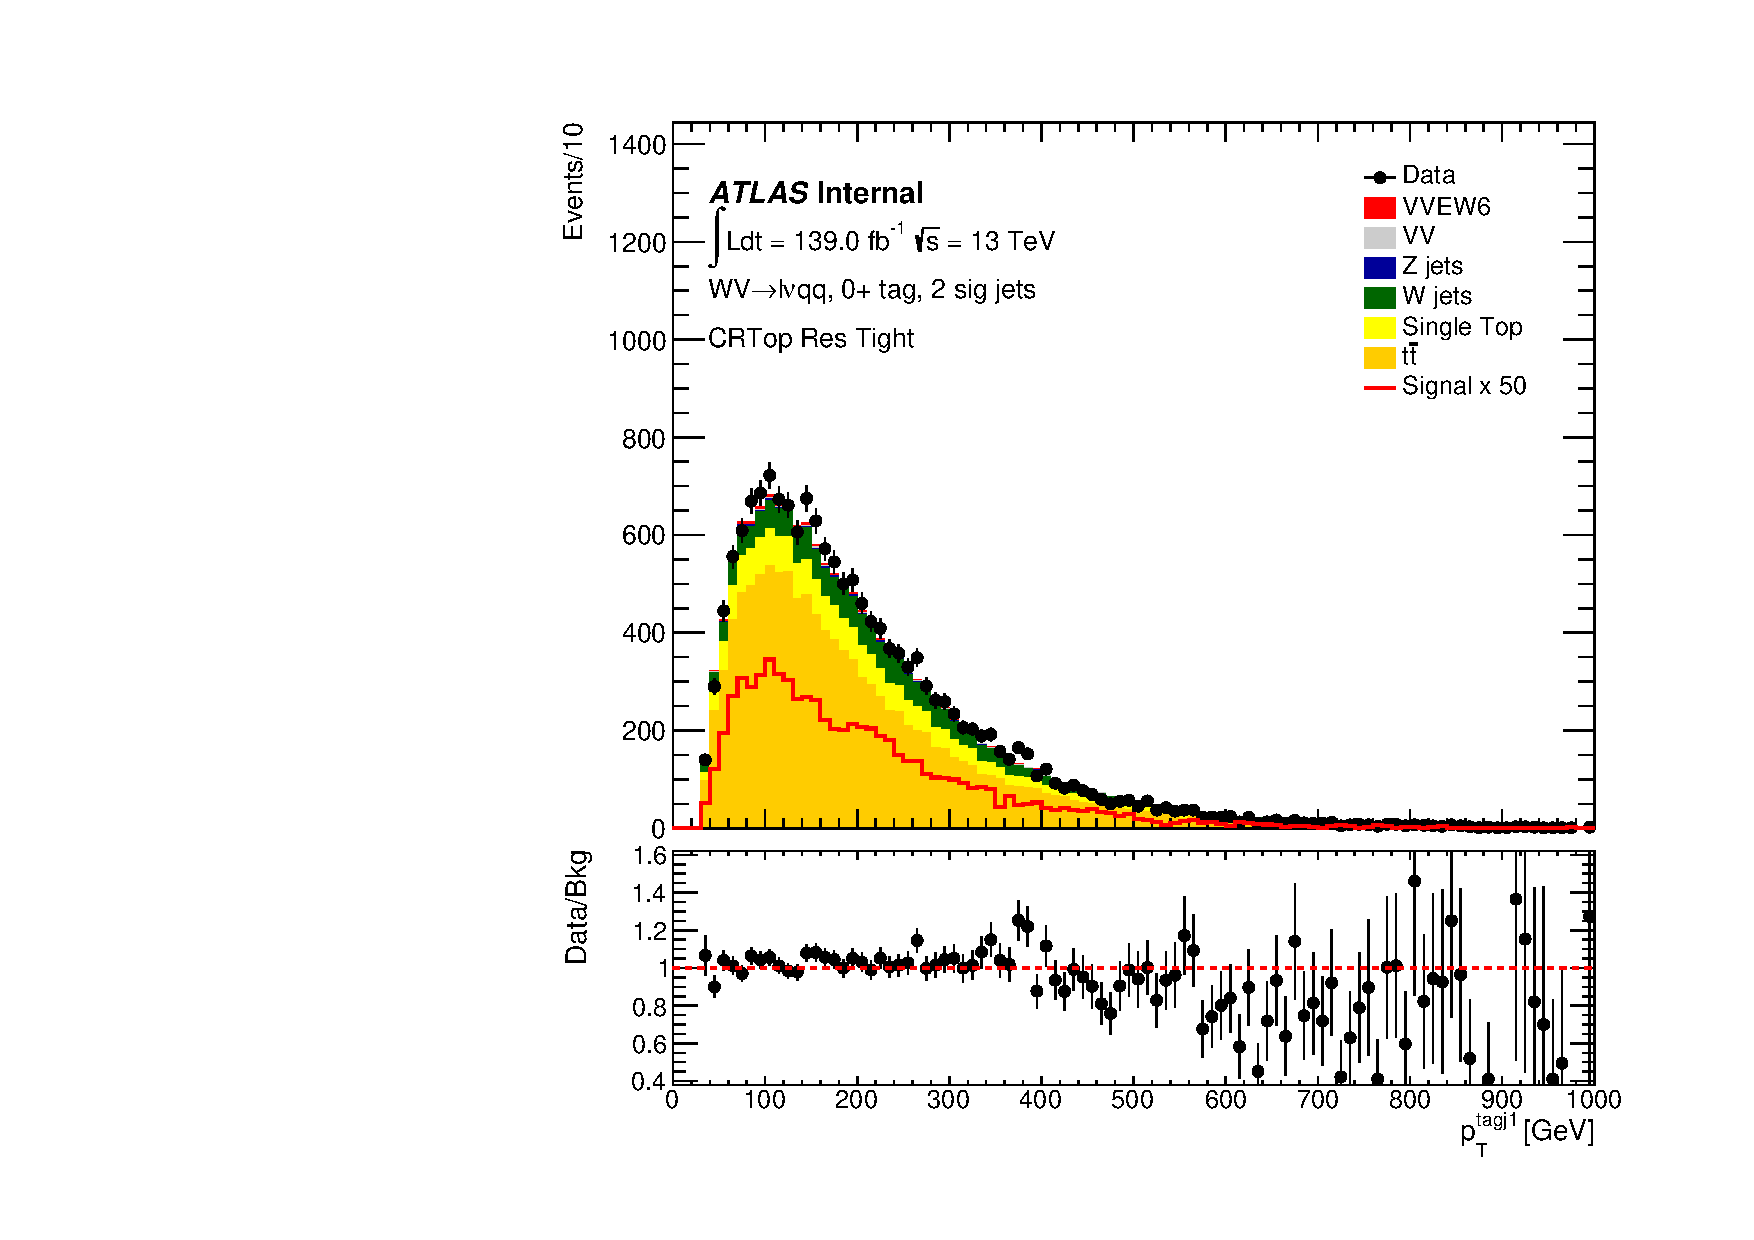
\includegraphics[width=0.3\textwidth]{figures/CRPlots/CRTop_Res_Tight/stacked_plot_resolved_tagJ1_pt.pdf}}
    \subfloat[]{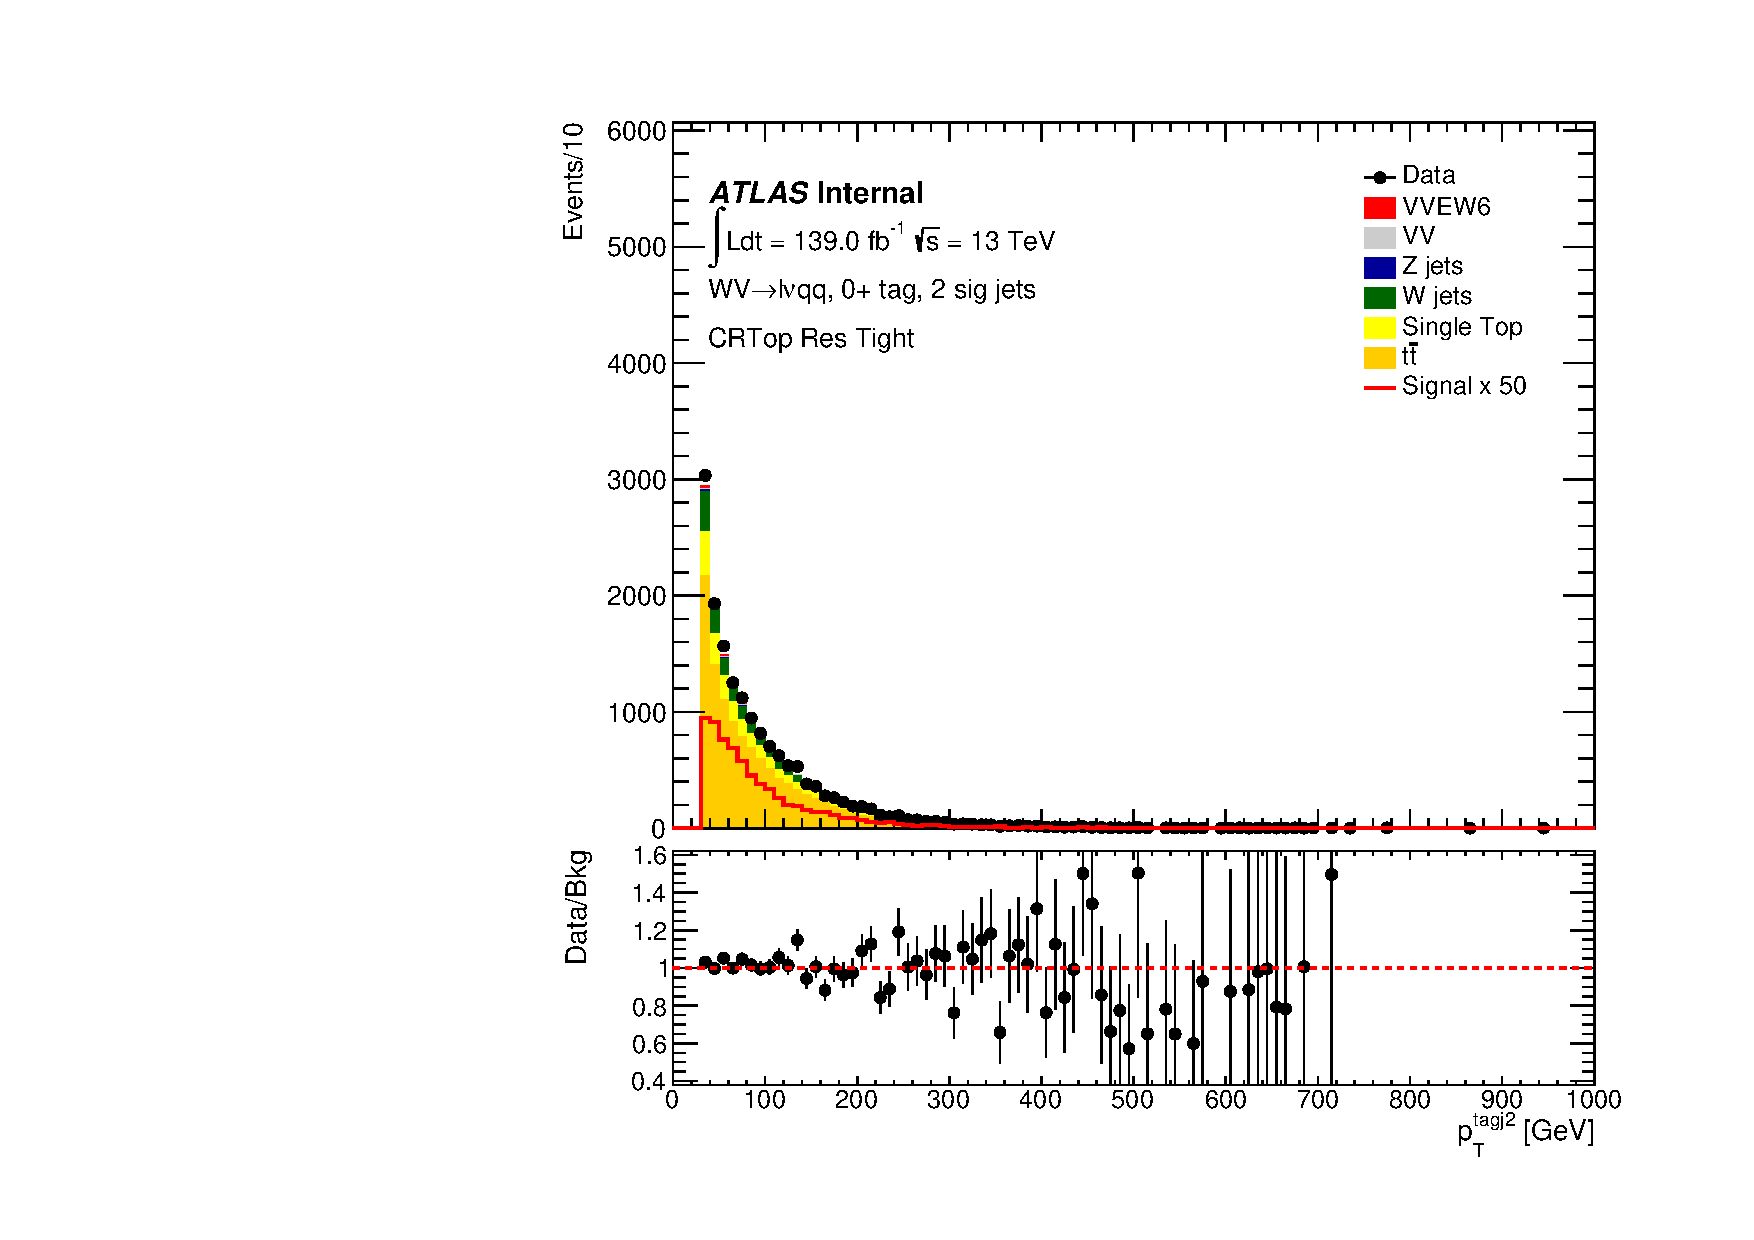
\includegraphics[width=0.3\textwidth]{figures/CRPlots/CRTop_Res_Tight/stacked_plot_resolved_tagJ2_pt.pdf}} \\
    \subfloat[]{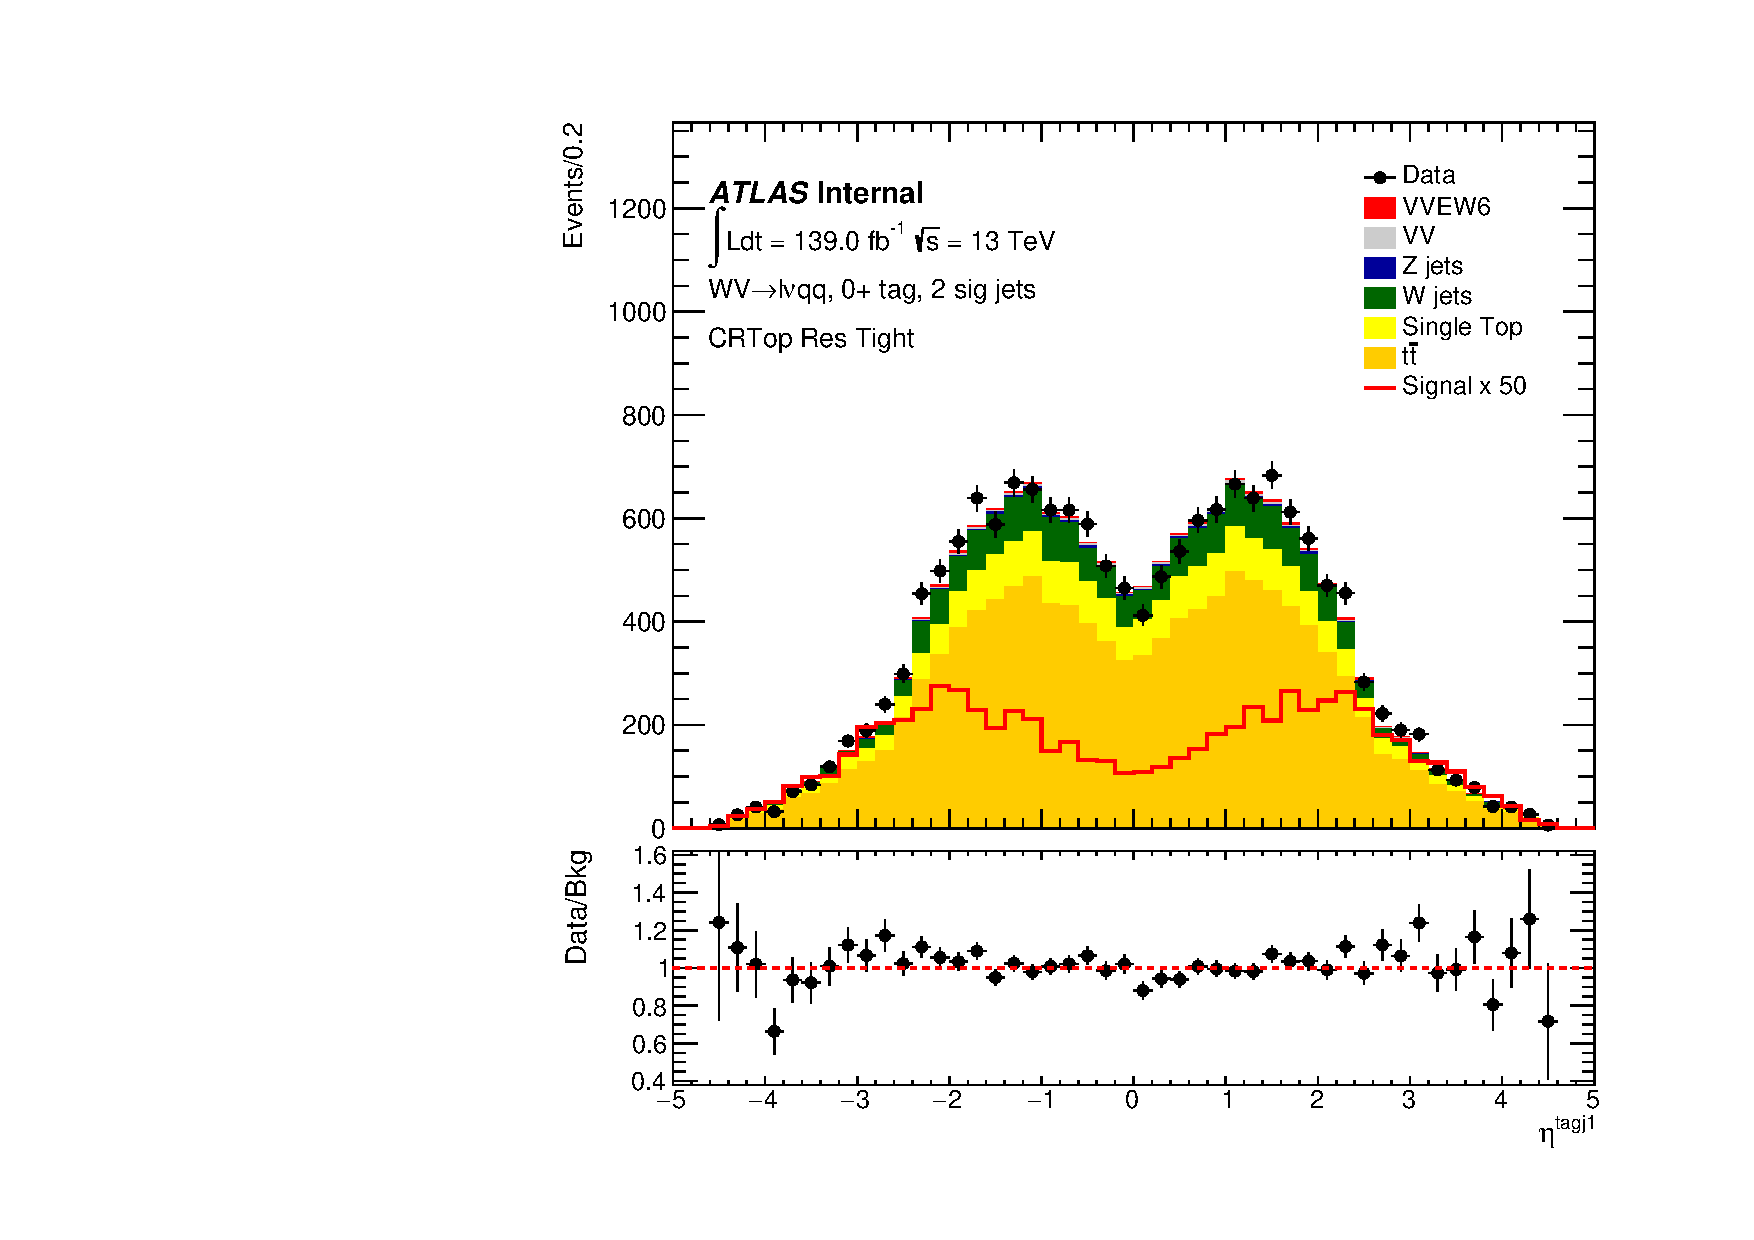
\includegraphics[width=0.3\textwidth]{figures/CRPlots/CRTop_Res_Tight/stacked_plot_resolved_tagJ1_eta.pdf}}
    \subfloat[]{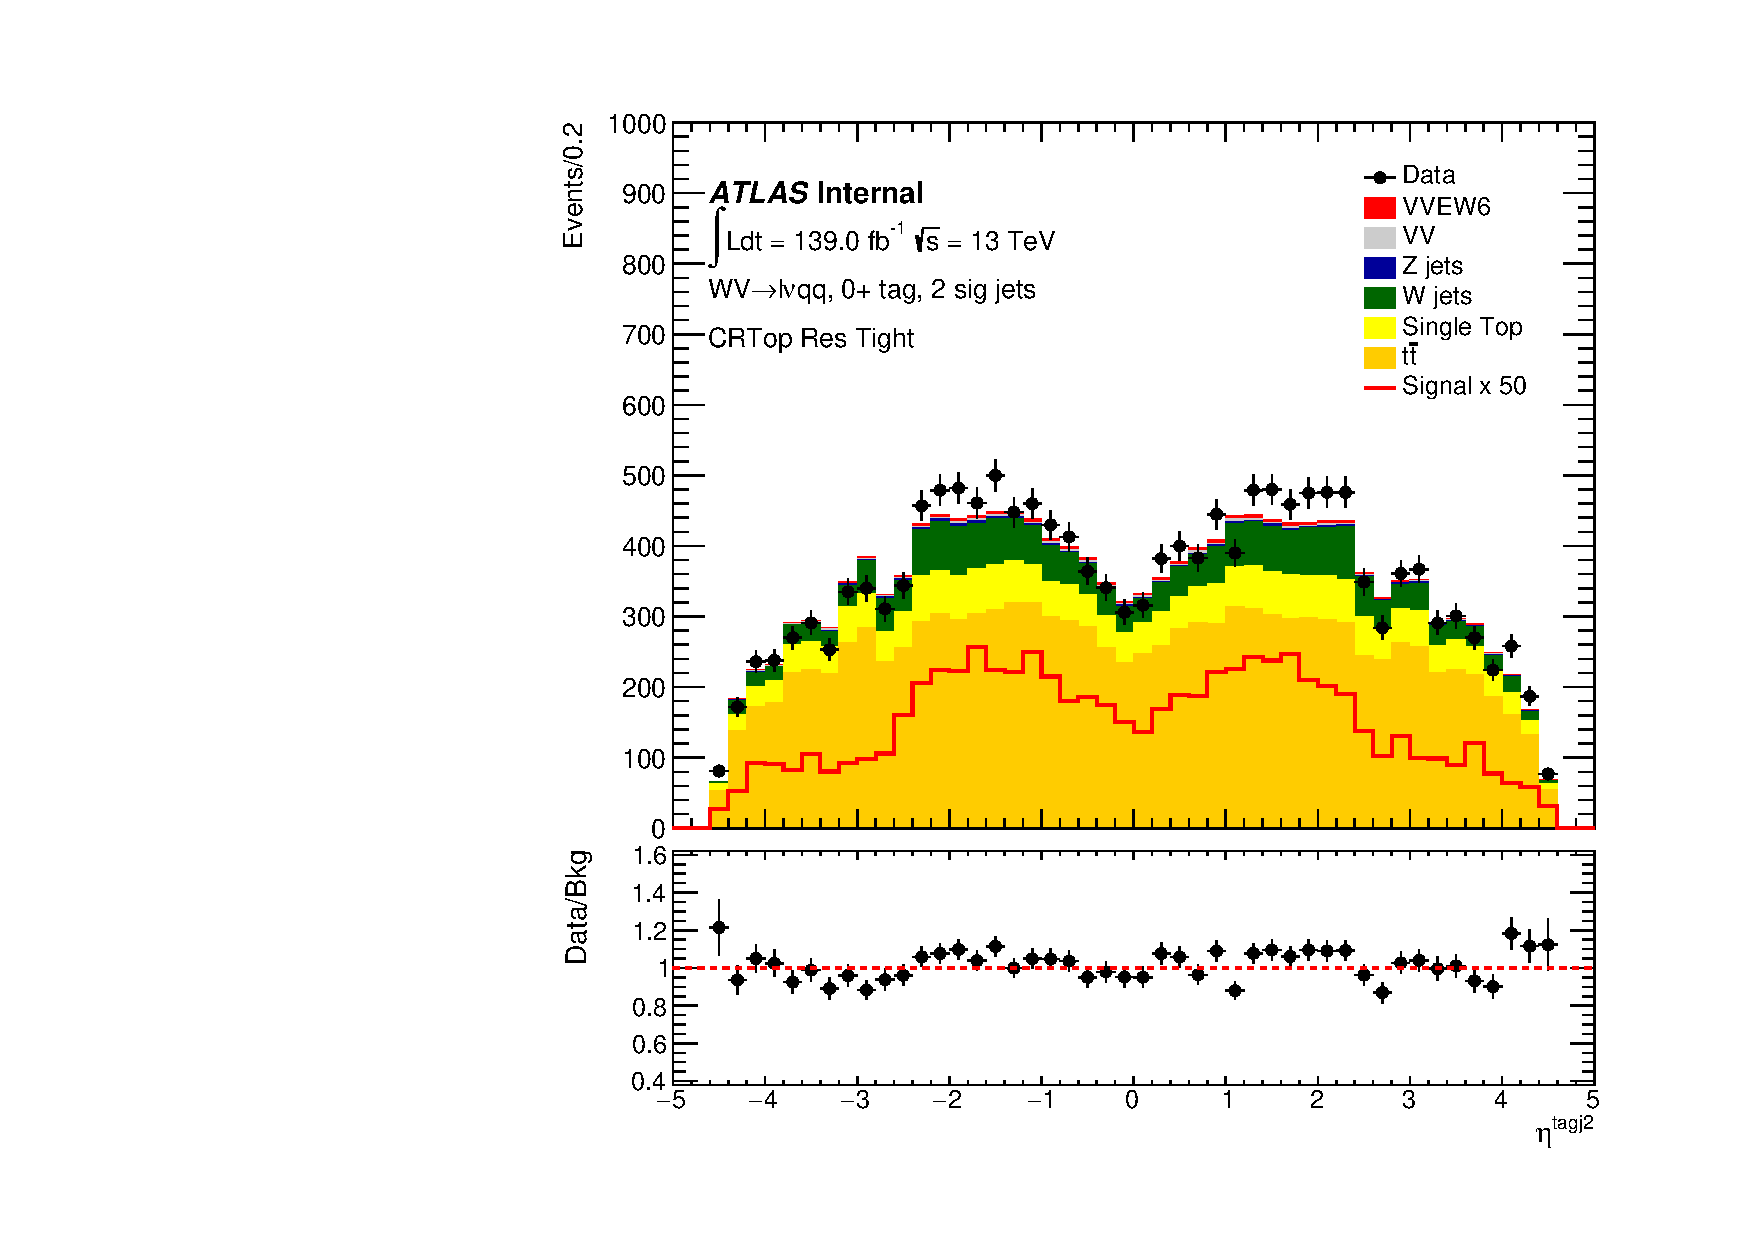
\includegraphics[width=0.3\textwidth]{figures/CRPlots/CRTop_Res_Tight/stacked_plot_resolved_tagJ2_eta.pdf}} \\
    \subfloat[]{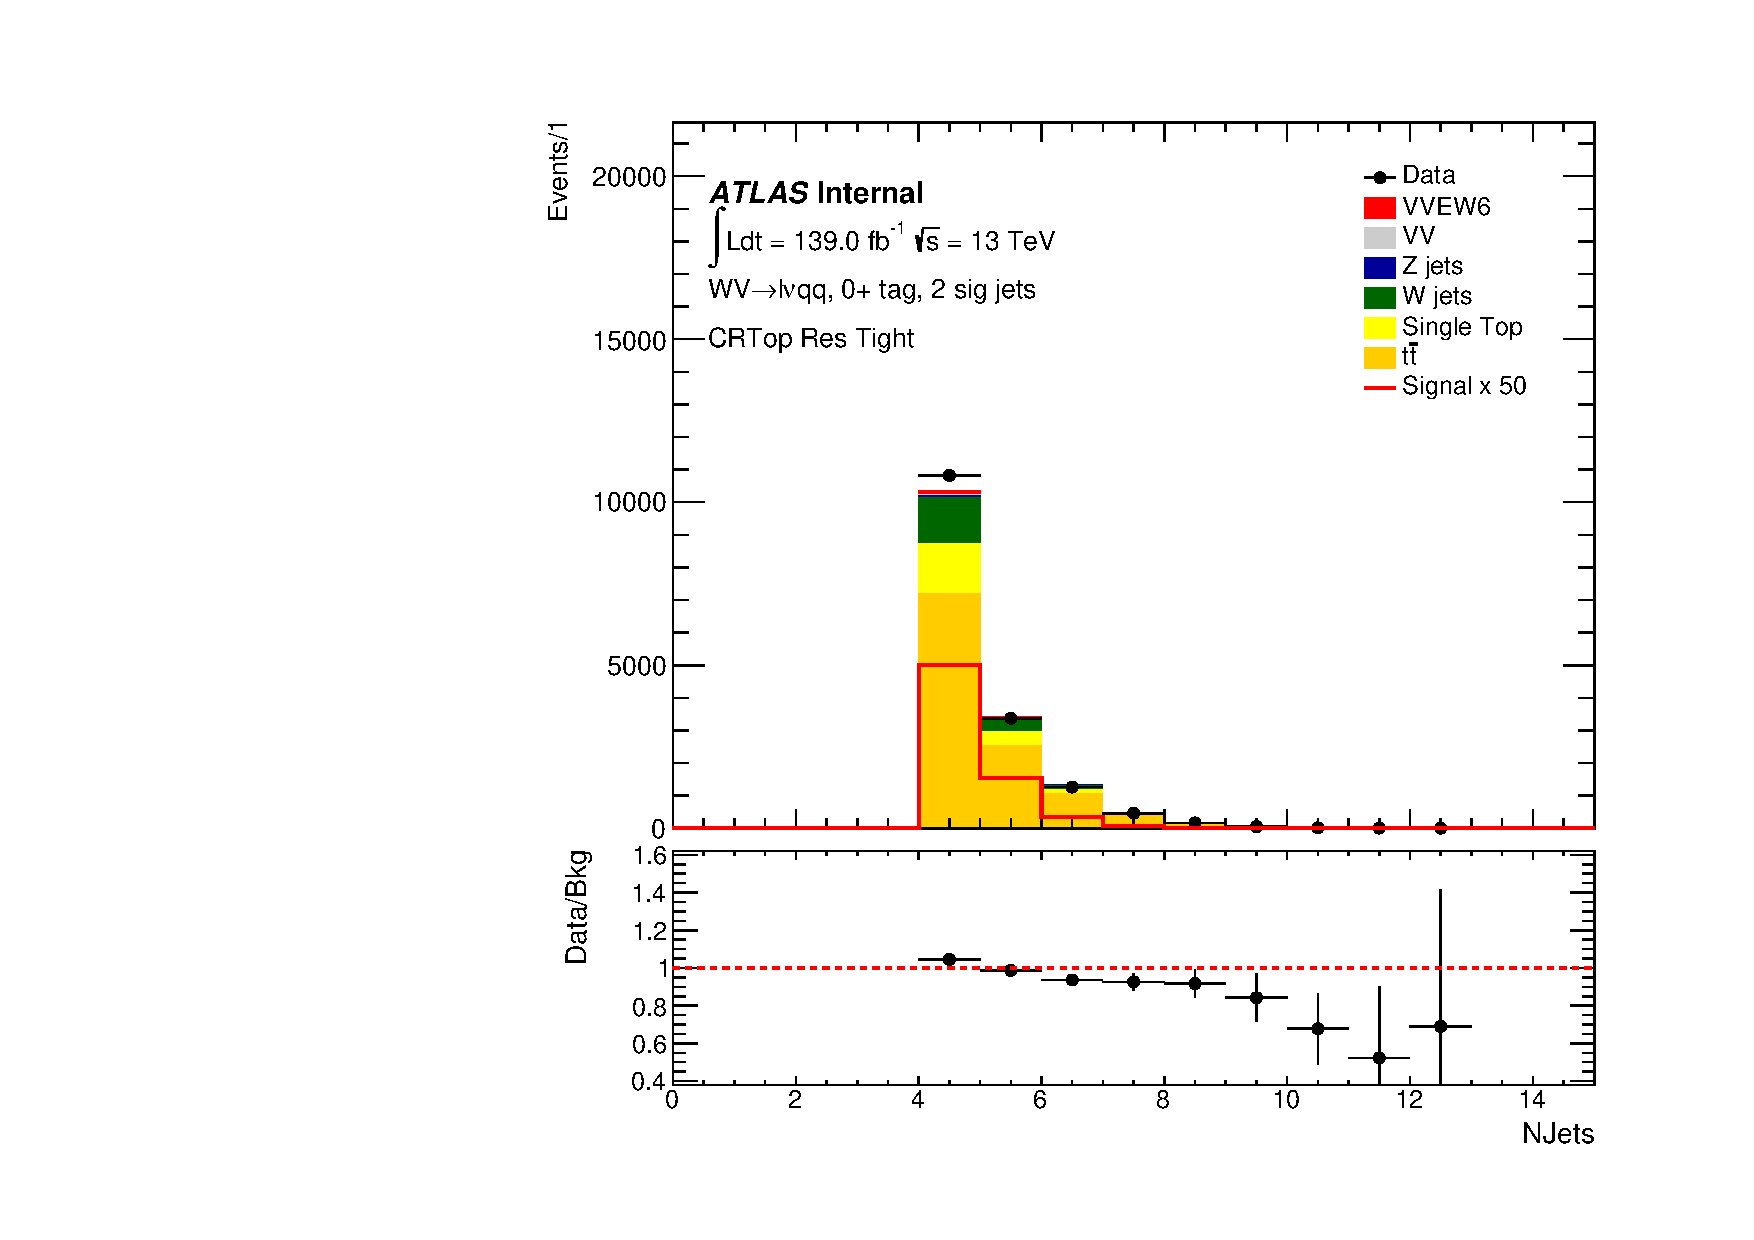
\includegraphics[width=0.3\textwidth]{figures/CRPlots/CRTop_Res_Tight/stacked_plot_NJets.pdf}}
    \subfloat[]{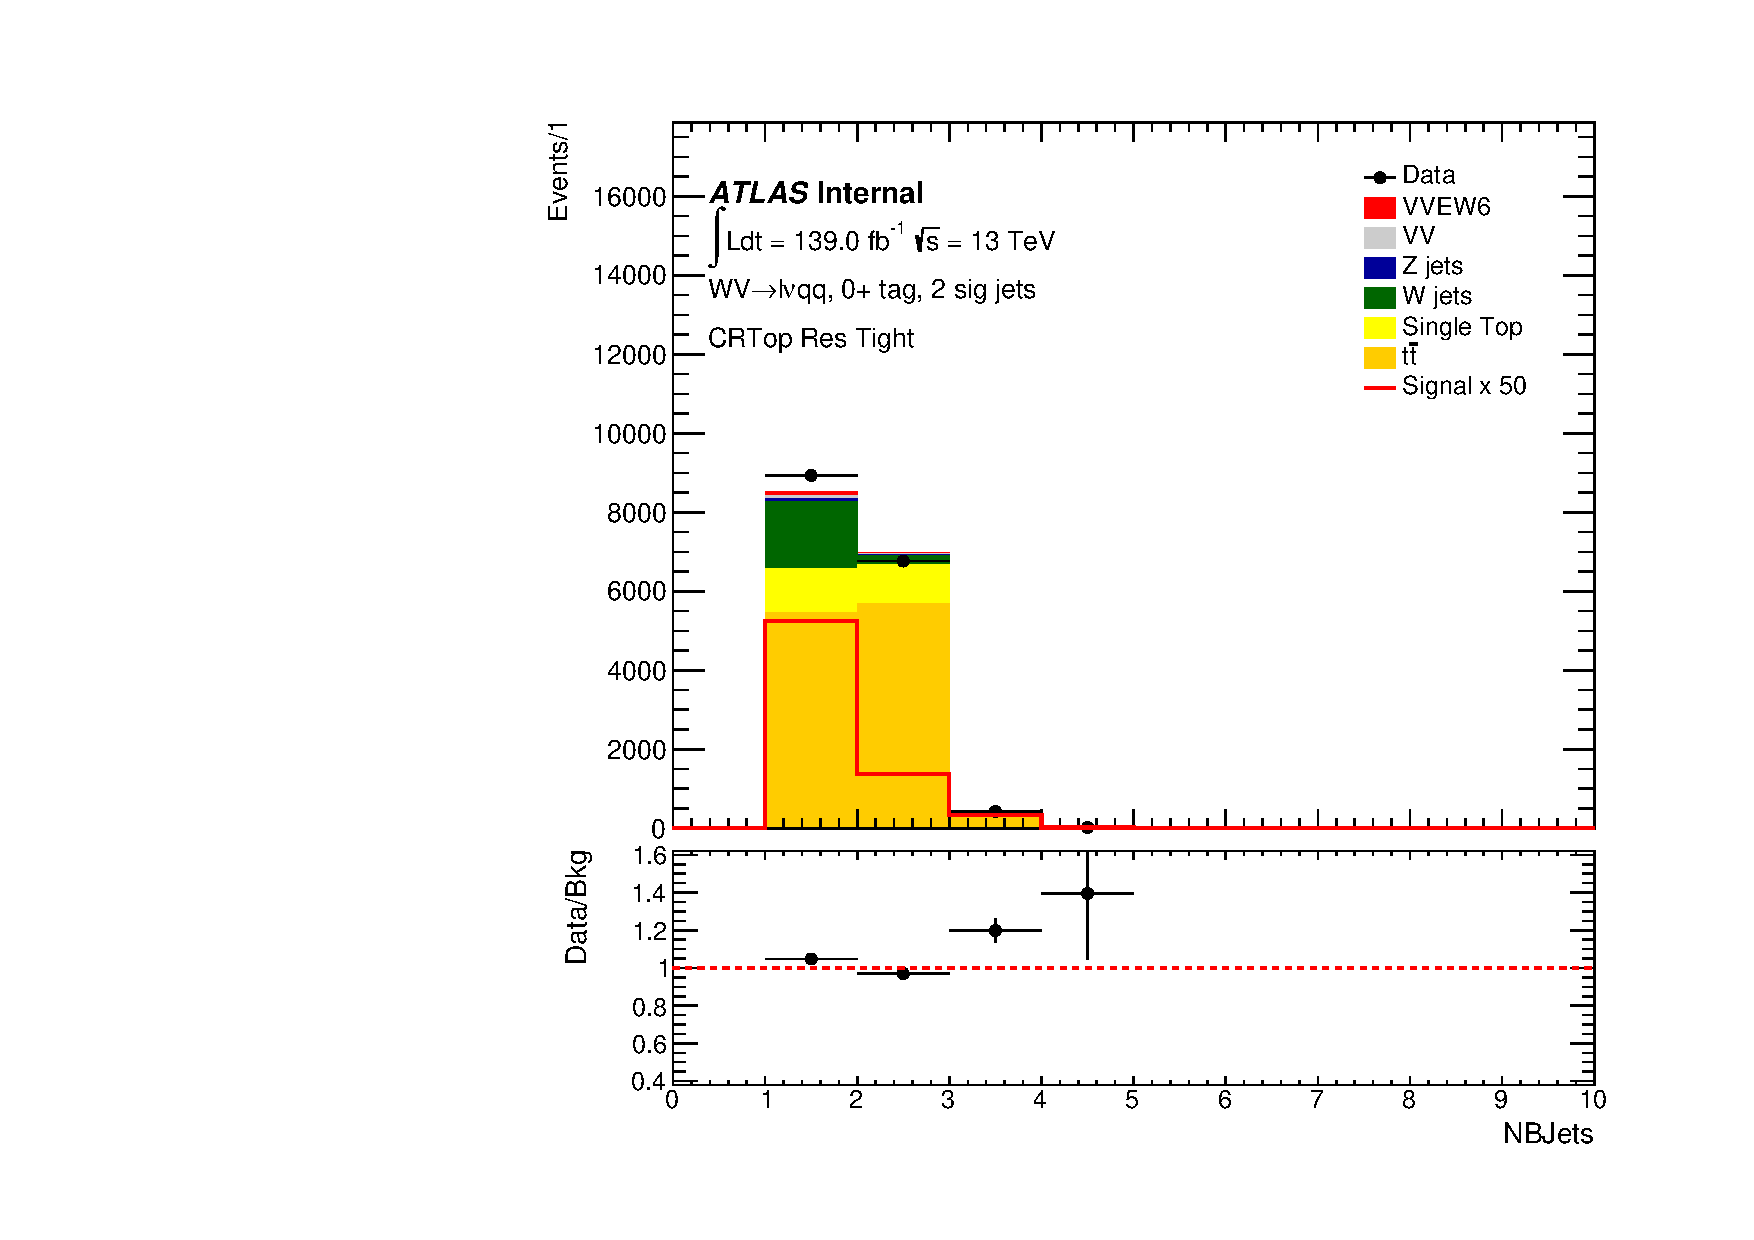
\includegraphics[width=0.3\textwidth]{figures/CRPlots/CRTop_Res_Tight/stacked_plot_NBJets.pdf}}
    \subfloat[]{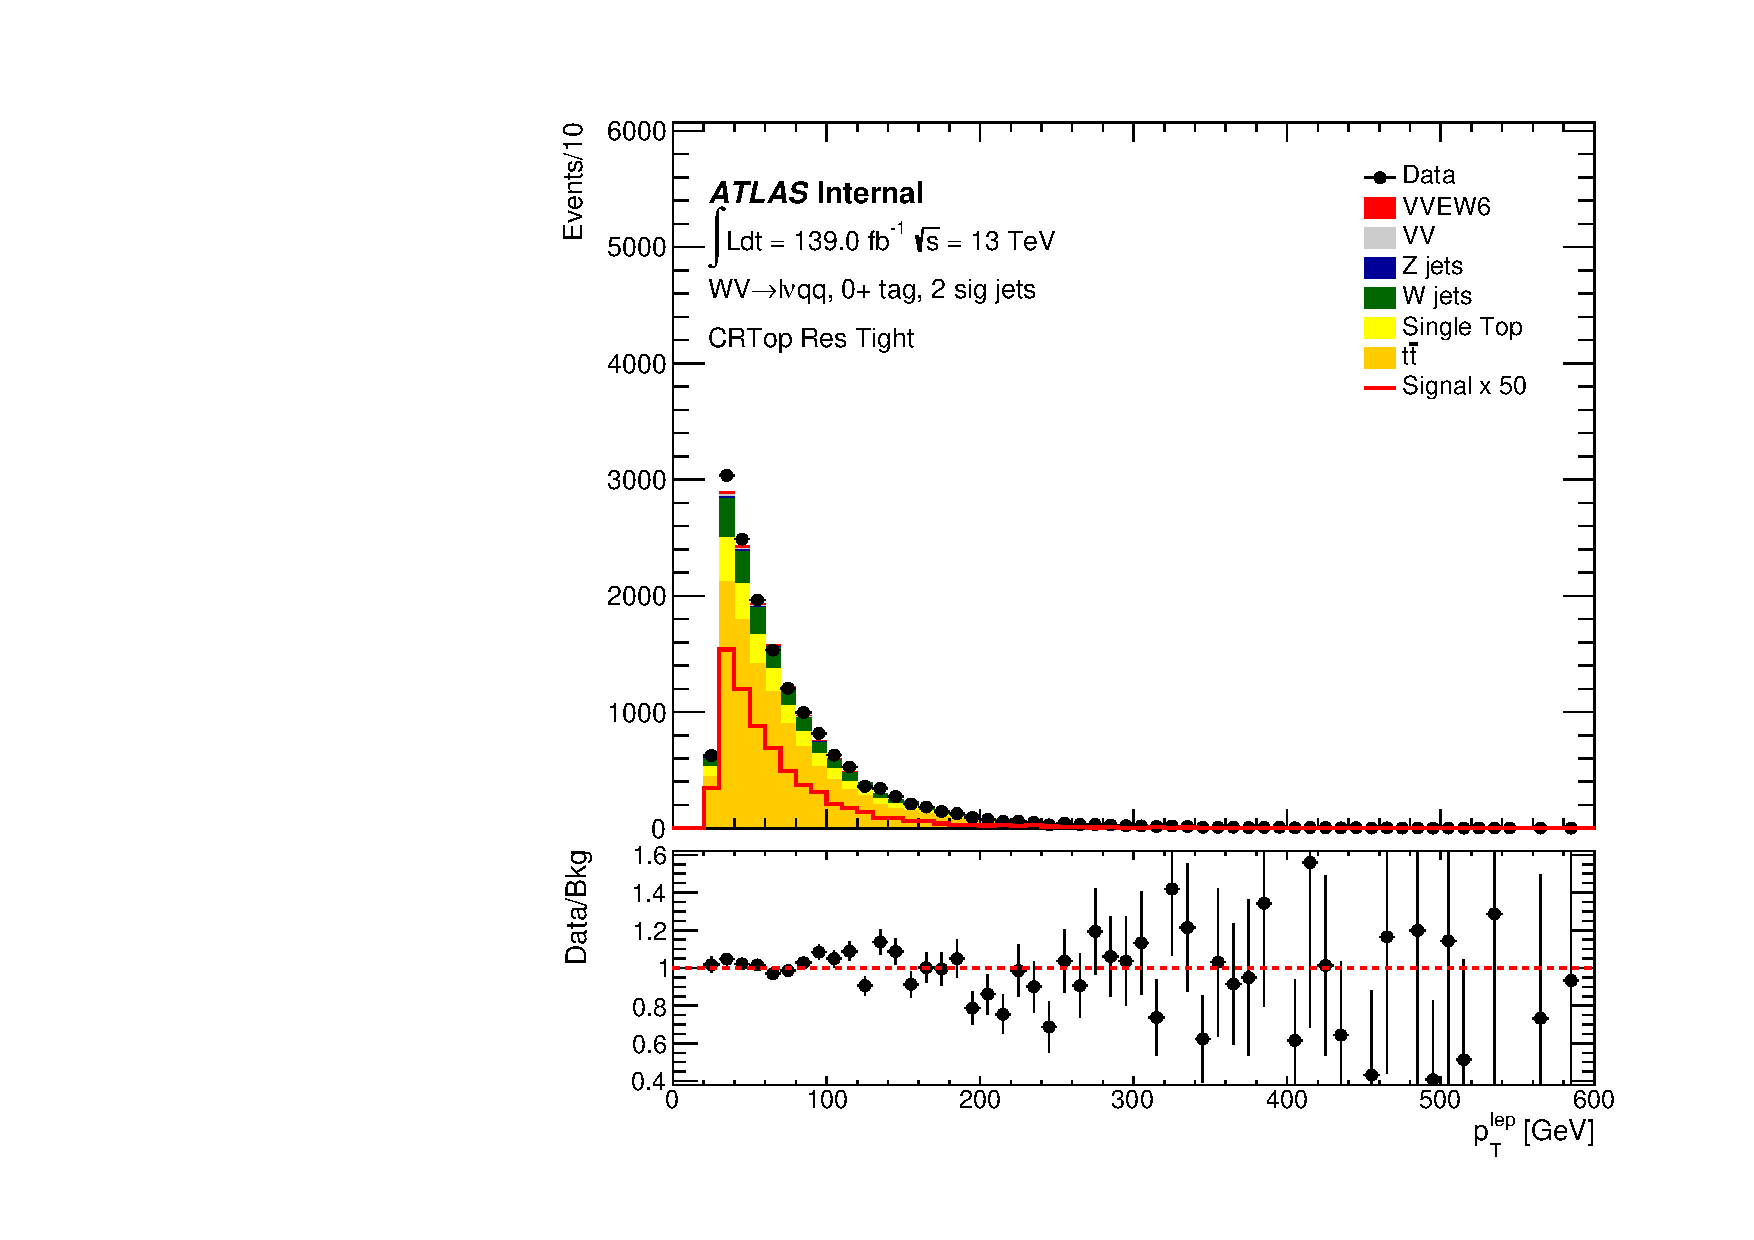
\includegraphics[width=0.3\textwidth]{figures/CRPlots/CRTop_Res_Tight/stacked_plot_lep_pt.pdf}}
    \caption{Data-MC checks for the resolved tight top control region in the \olep channel.}
    \label{fig:CRTopResTightPlots1Lep}
\end{figure}

\begin{figure}[ht]
    \centering
    \subfloat[]{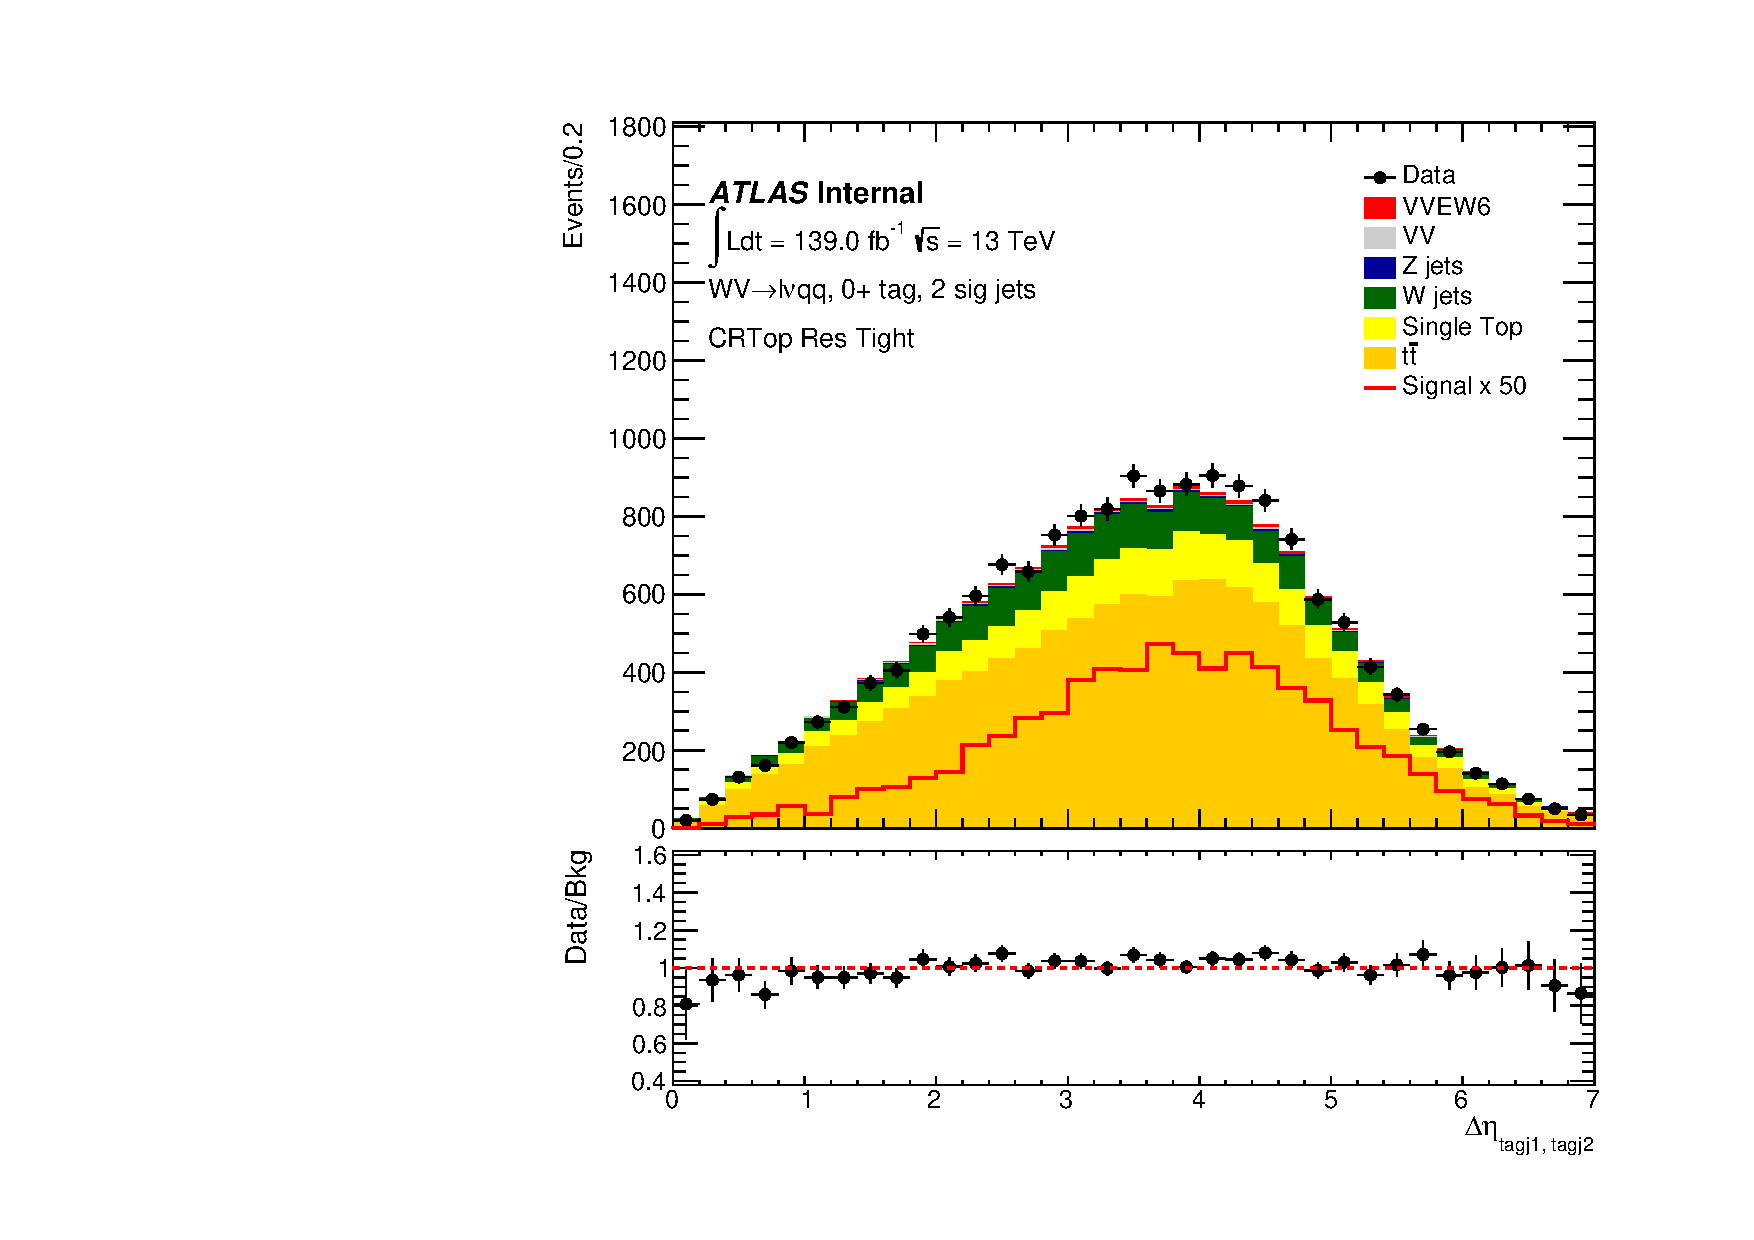
\includegraphics[width=0.3\textwidth]{figures/CRPlots/CRTop_Res_Tight/stacked_plot_resolved_tagJdEta.pdf}}
    \subfloat[]{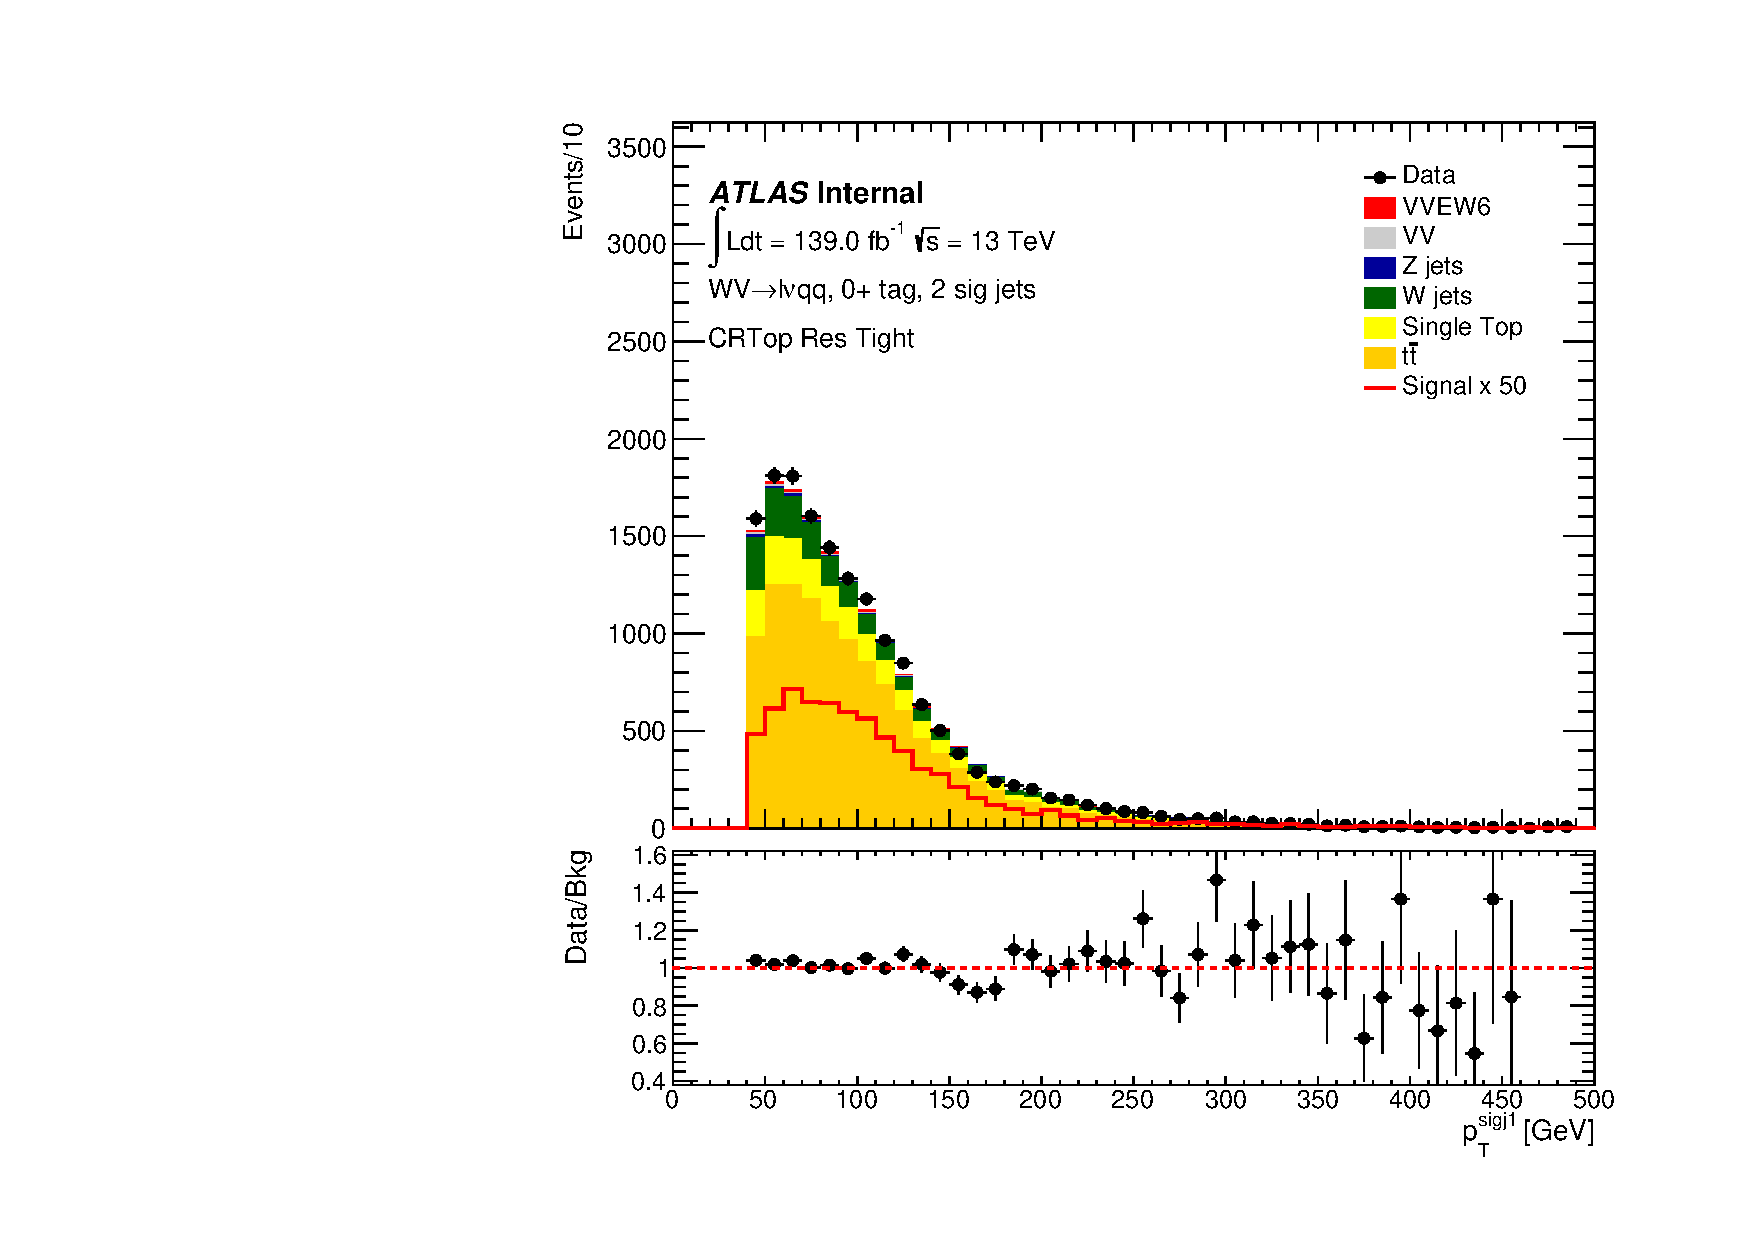
\includegraphics[width=0.3\textwidth]{figures/CRPlots/CRTop_Res_Tight/stacked_plot_sigJ1_pt.pdf}}
    \subfloat[]{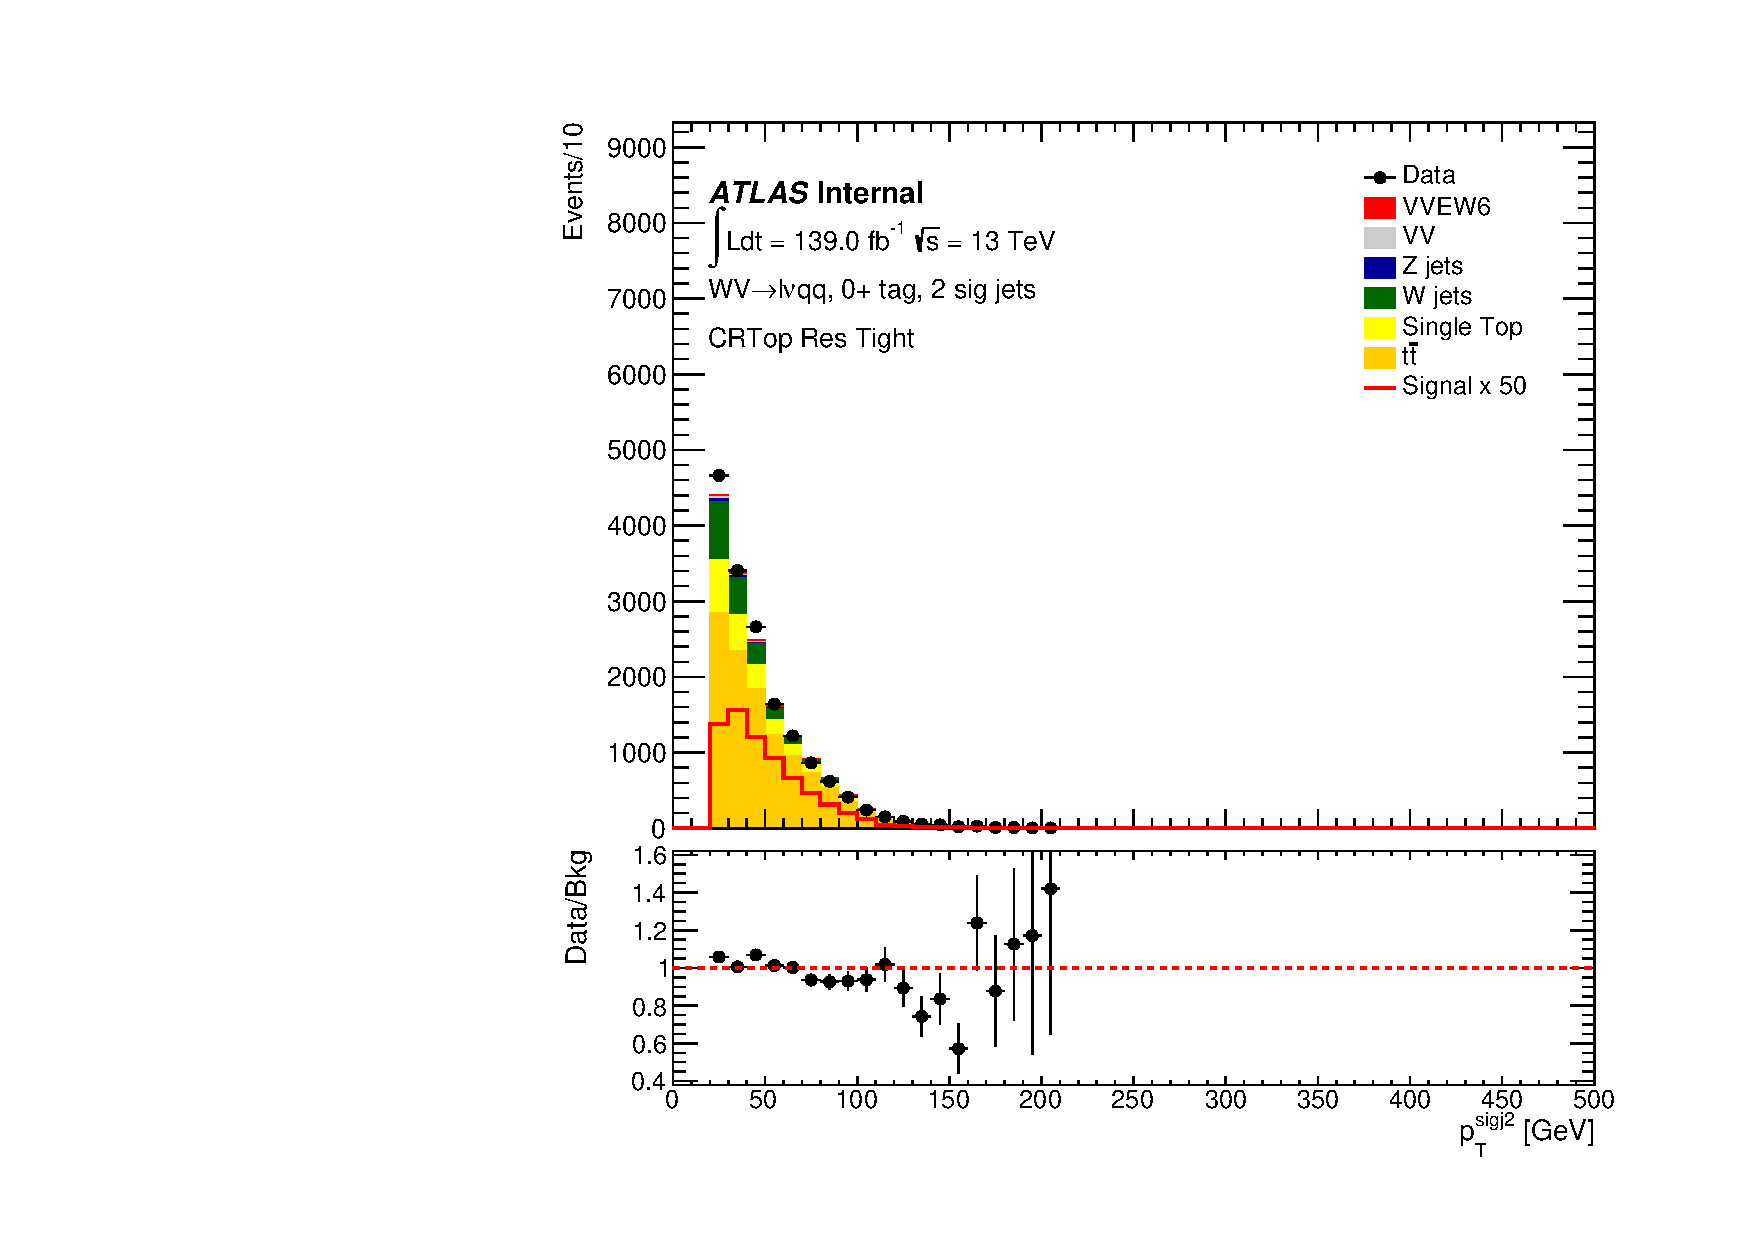
\includegraphics[width=0.3\textwidth]{figures/CRPlots/CRTop_Res_Tight/stacked_plot_sigJ2_pt.pdf}} \\
    \subfloat[]{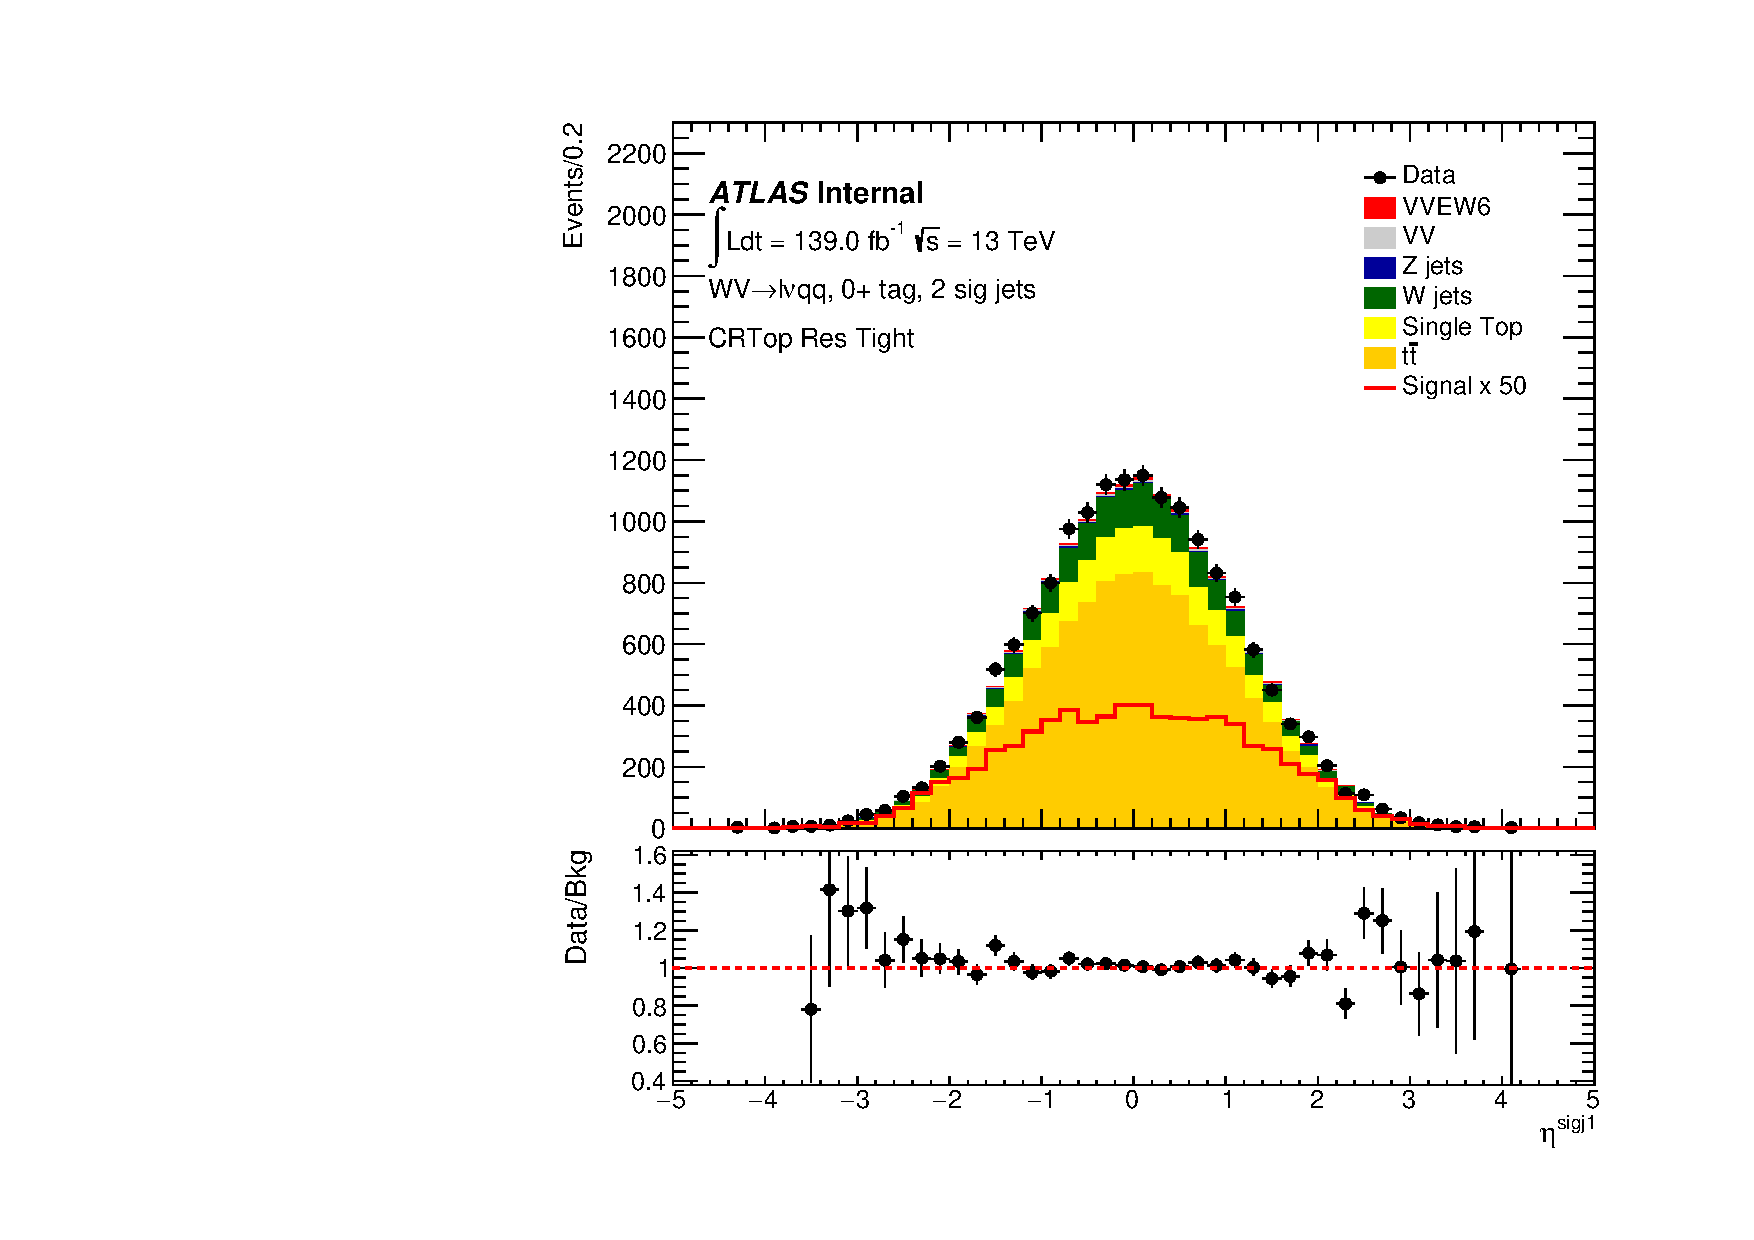
\includegraphics[width=0.3\textwidth]{figures/CRPlots/CRTop_Res_Tight/stacked_plot_sigJ1_eta.pdf}}
    \subfloat[]{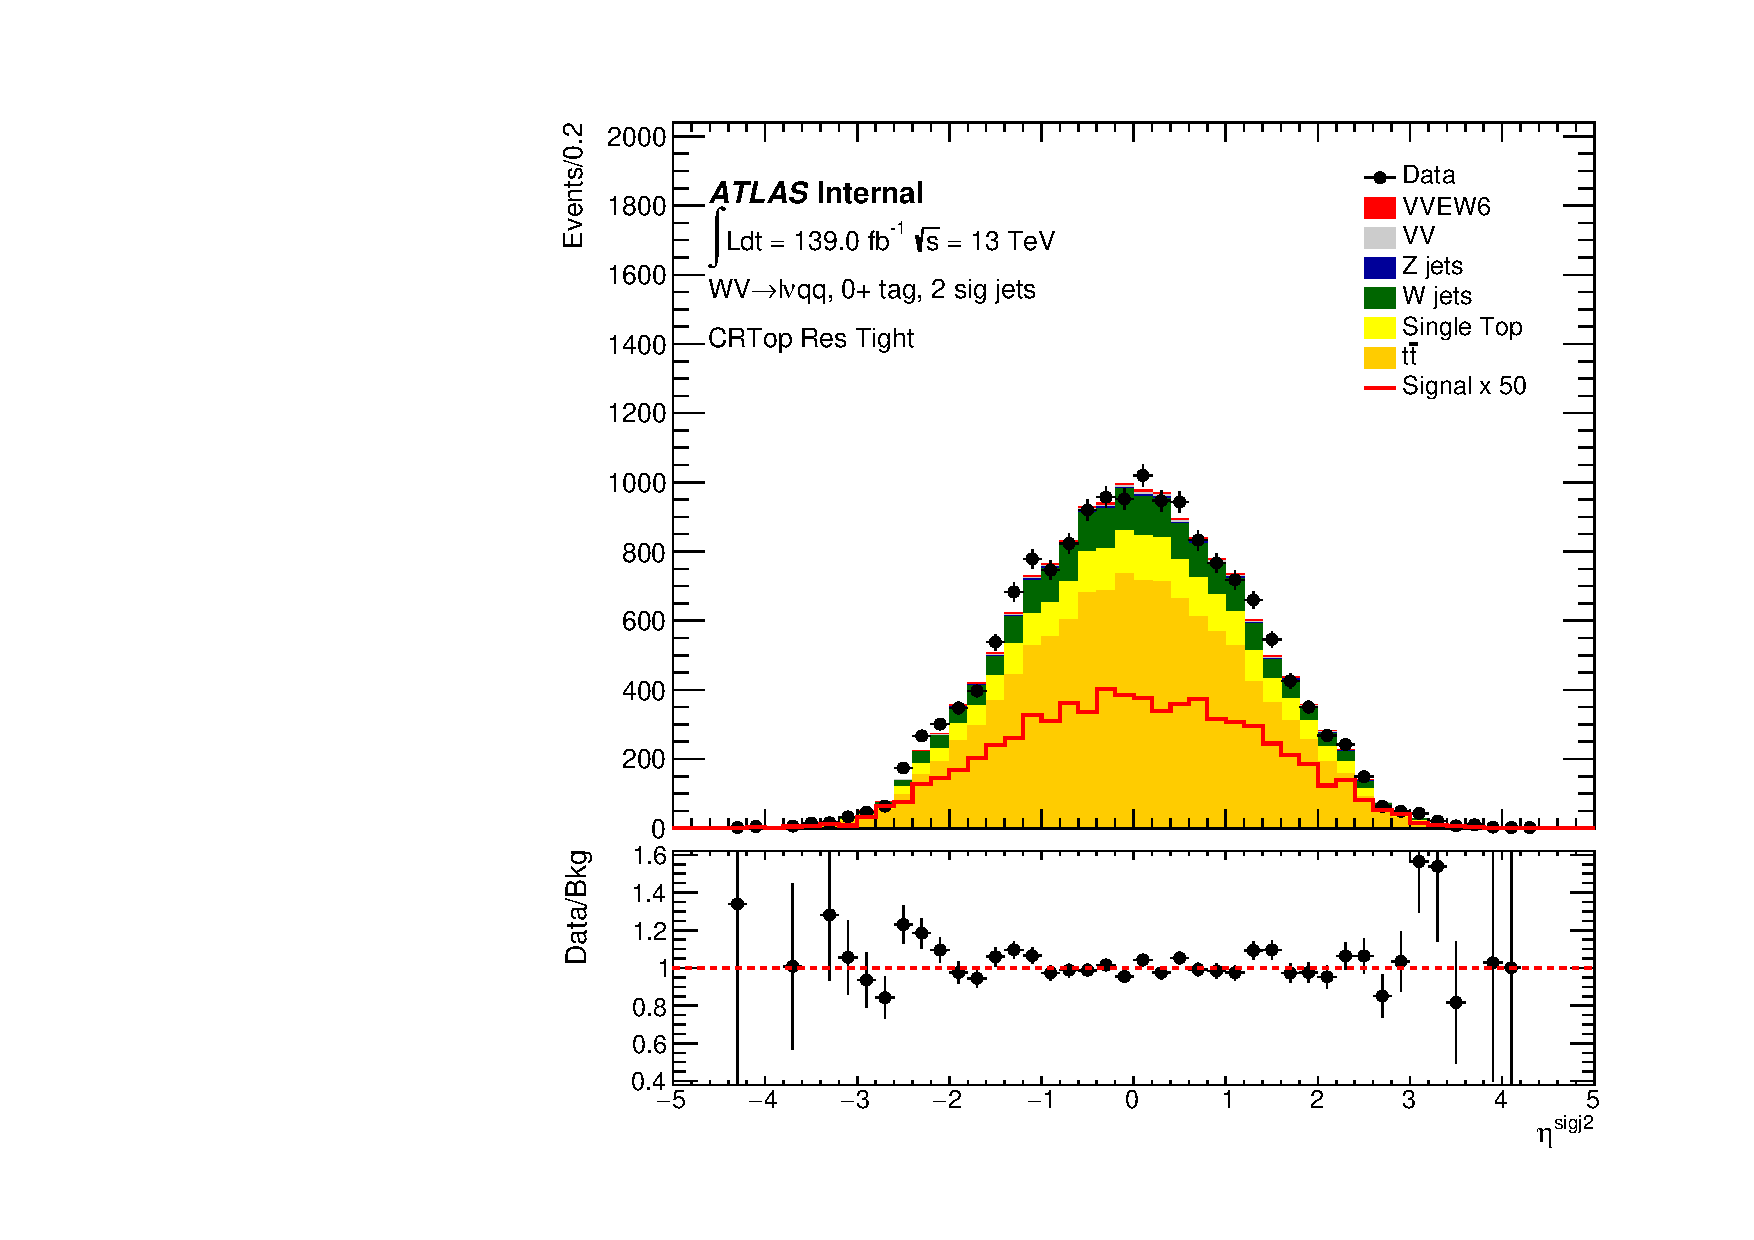
\includegraphics[width=0.3\textwidth]{figures/CRPlots/CRTop_Res_Tight/stacked_plot_sigJ2_eta.pdf}} \\
    \subfloat[]{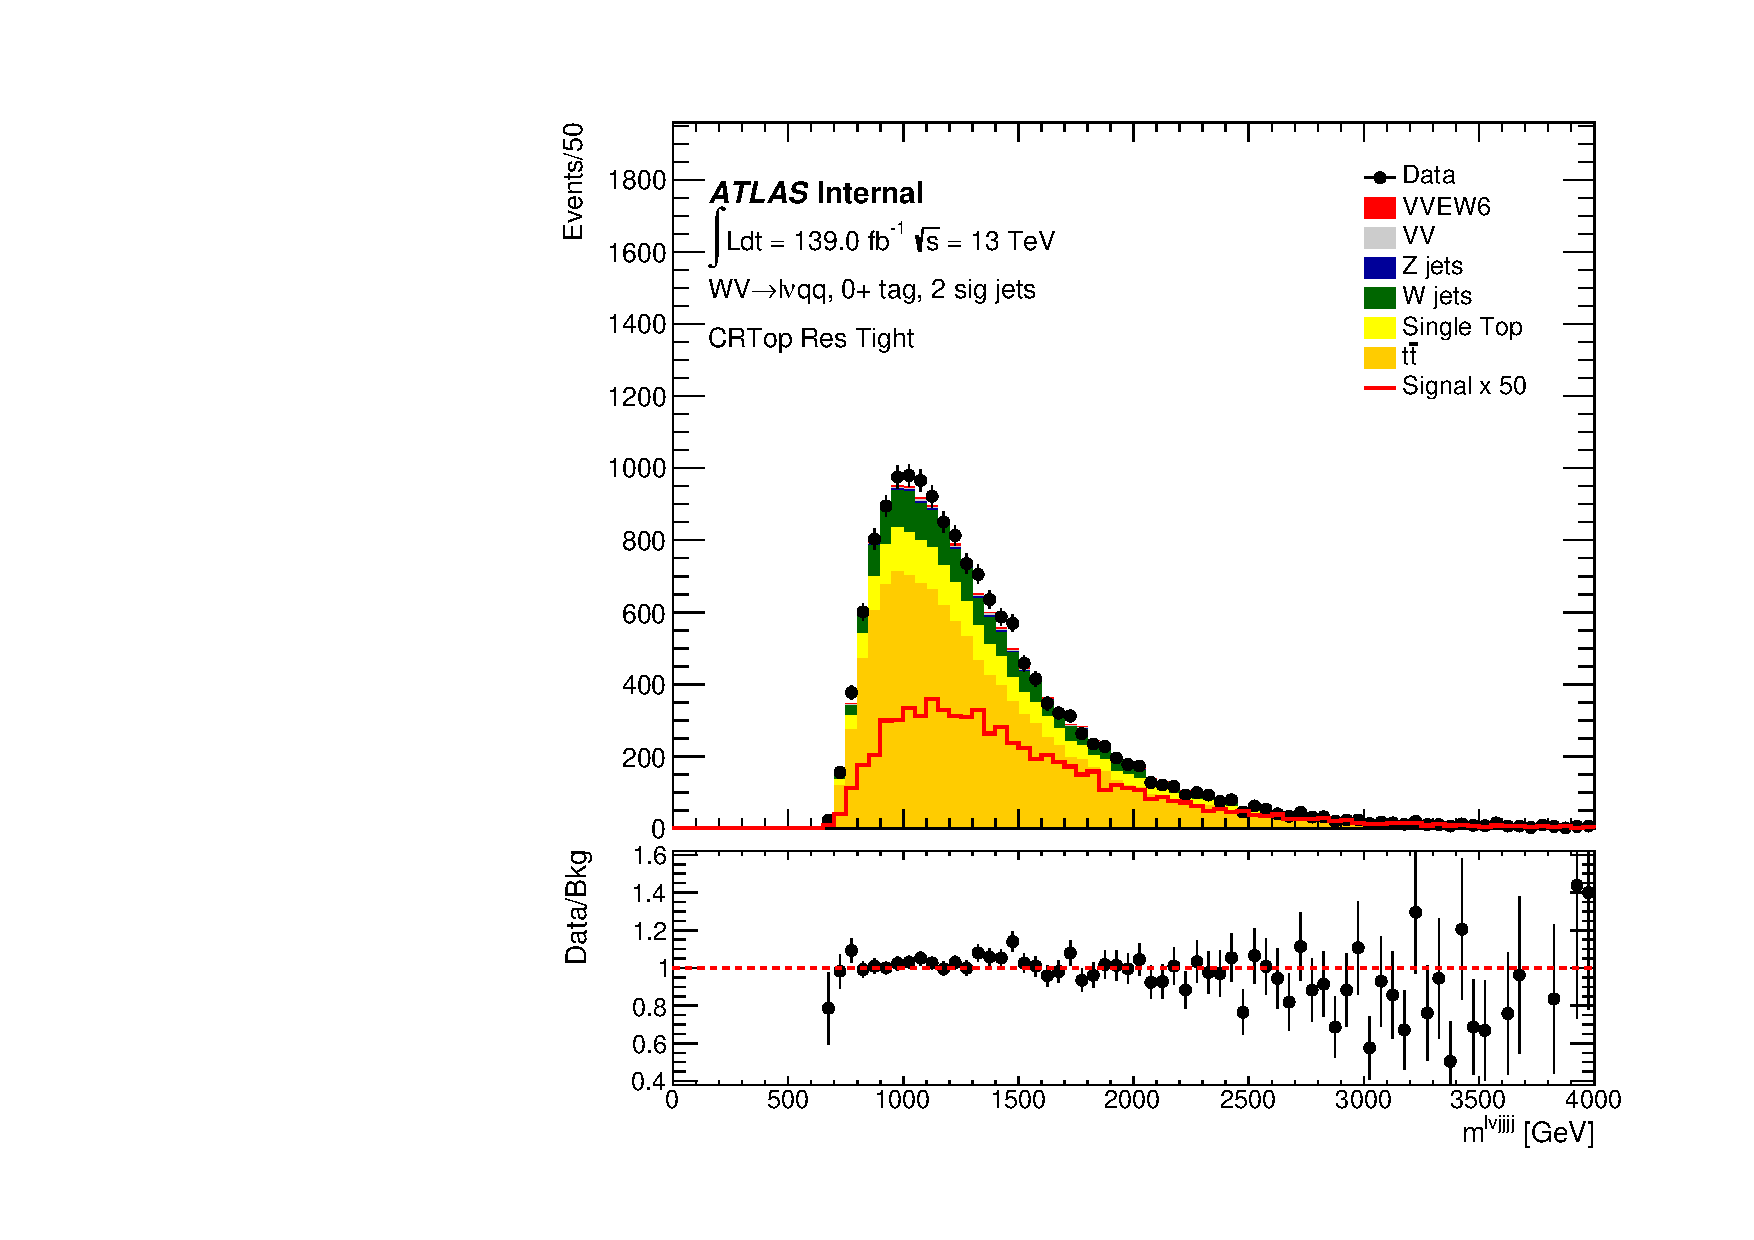
\includegraphics[width=0.3\textwidth]{figures/CRPlots/CRTop_Res_Tight/stacked_plot_lvjjjjmass.pdf}}
    \subfloat[]{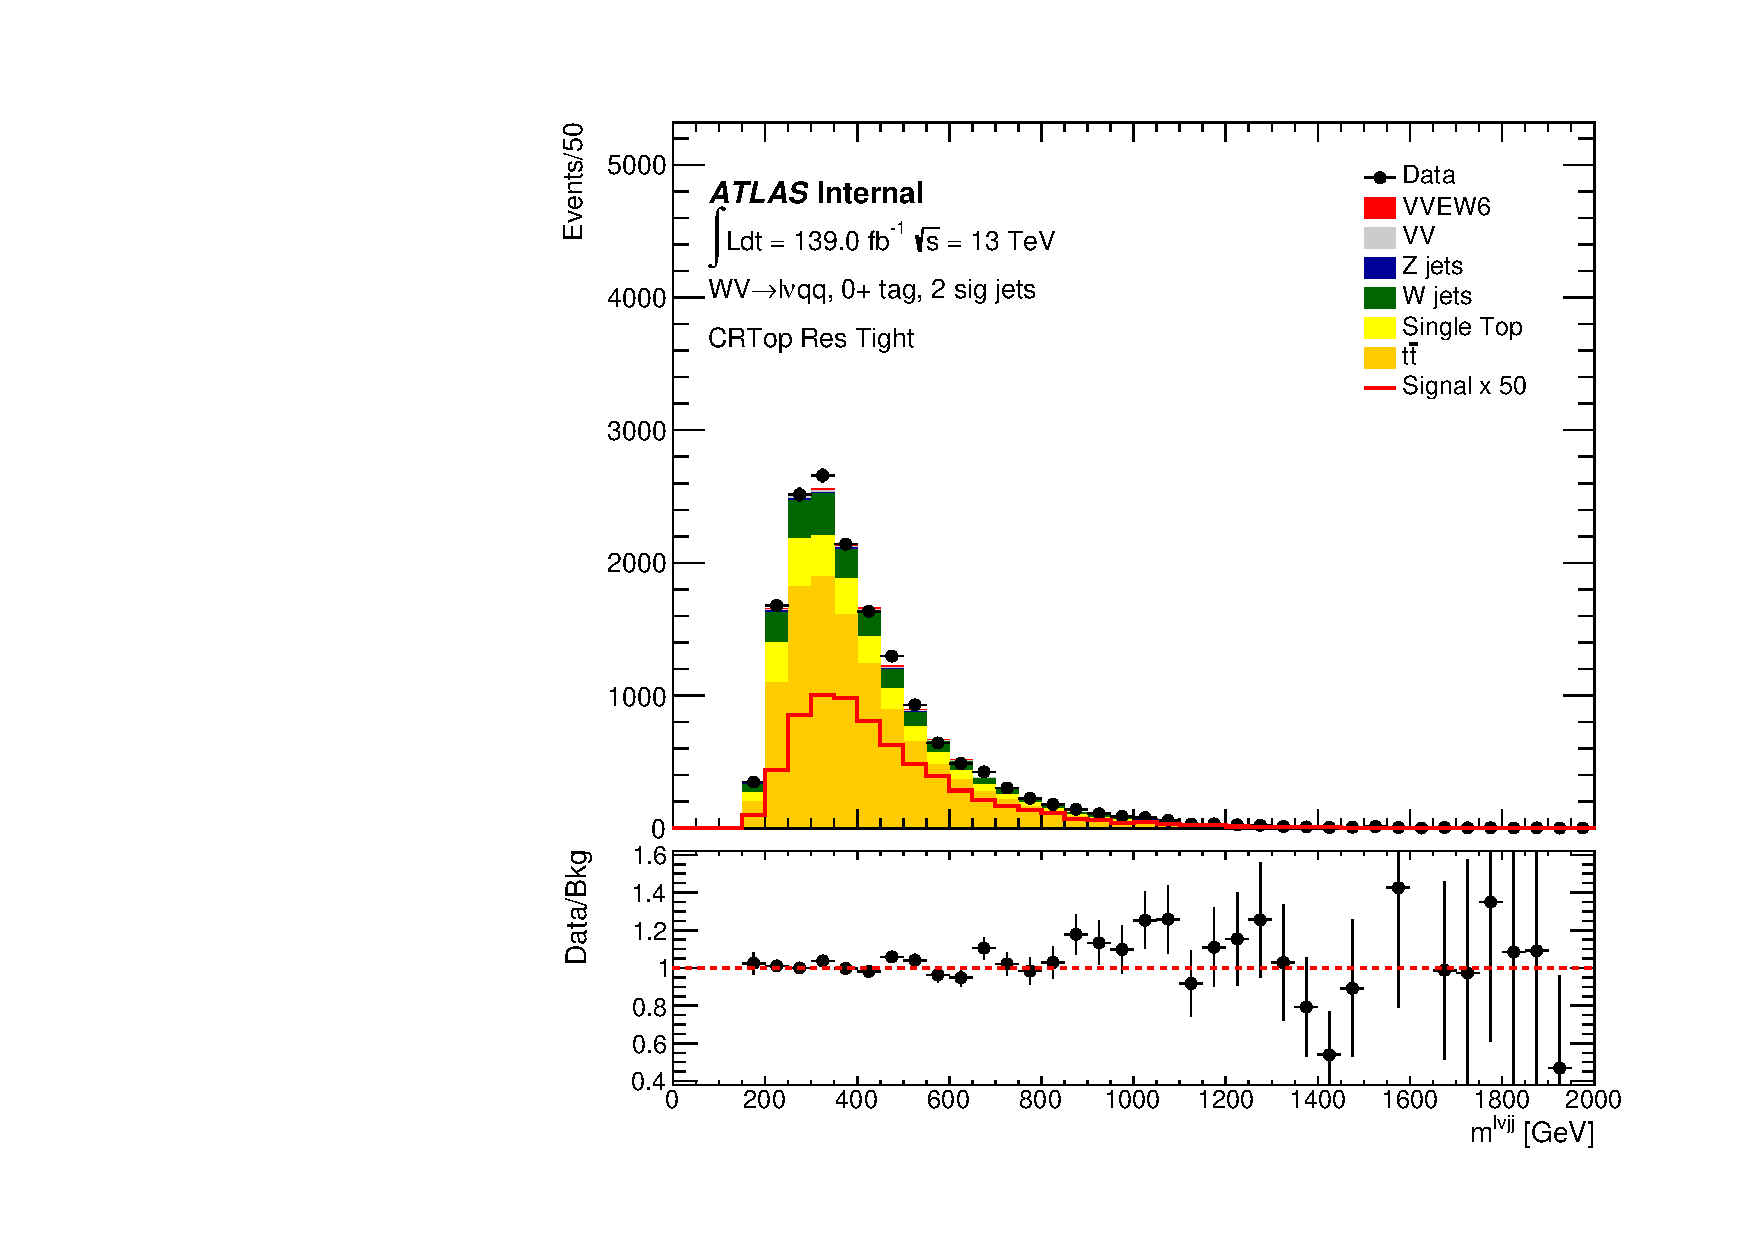
\includegraphics[width=0.3\textwidth]{figures/CRPlots/CRTop_Res_Tight/stacked_plot_lvjjmass.pdf}}
    \subfloat[]{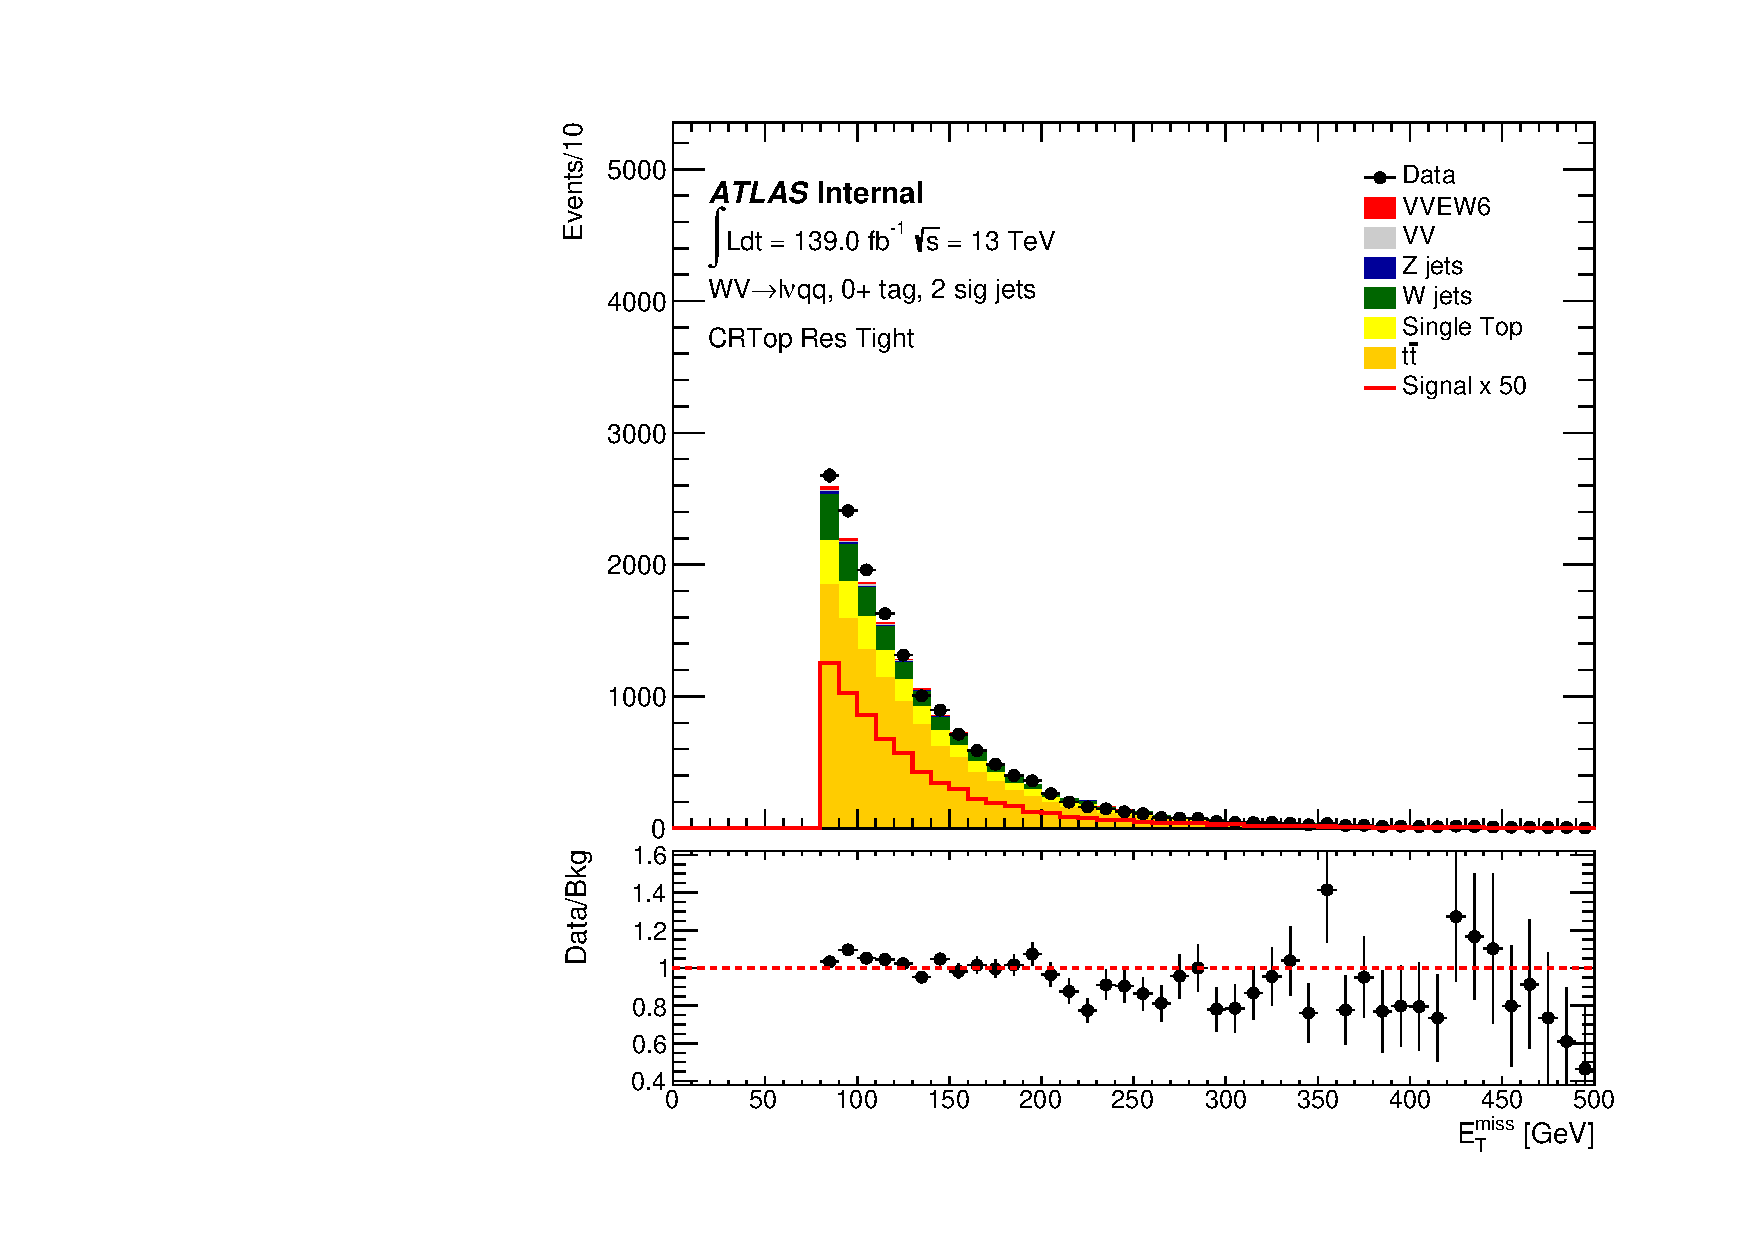
\includegraphics[width=0.3\textwidth]{figures/CRPlots/CRTop_Res_Tight/stacked_plot_met.pdf}}  \\
    \caption{Data-MC checks for the resolved tight top control region in the \olep channel.}
    \label{fig:CRTopResTightPlots1Lep2}
\end{figure}

\begin{figure}[ht]
    \centering
    \subfloat[]{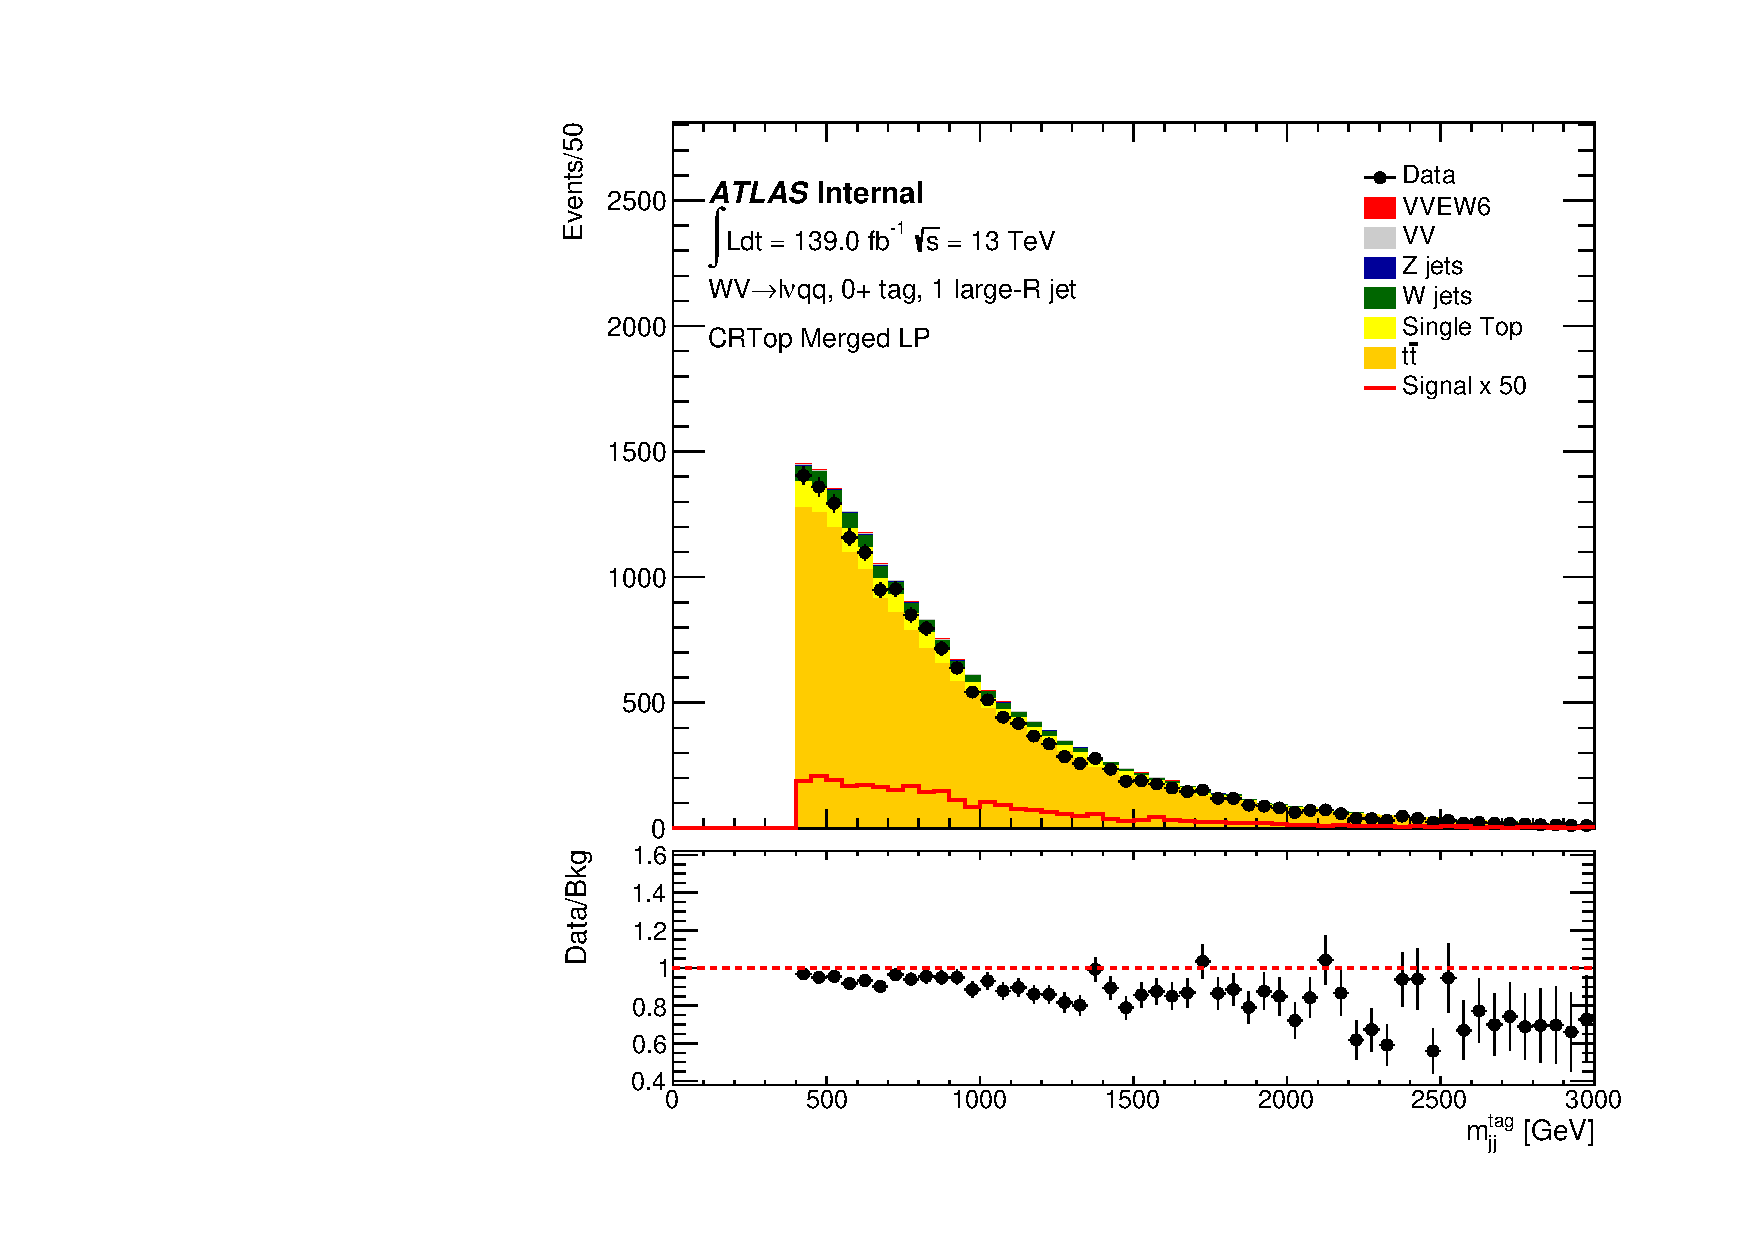
\includegraphics[width=0.3\textwidth]{figures/CRPlots/CRTop_80/stacked_plot_merged_tagMjj.pdf}}
    \subfloat[]{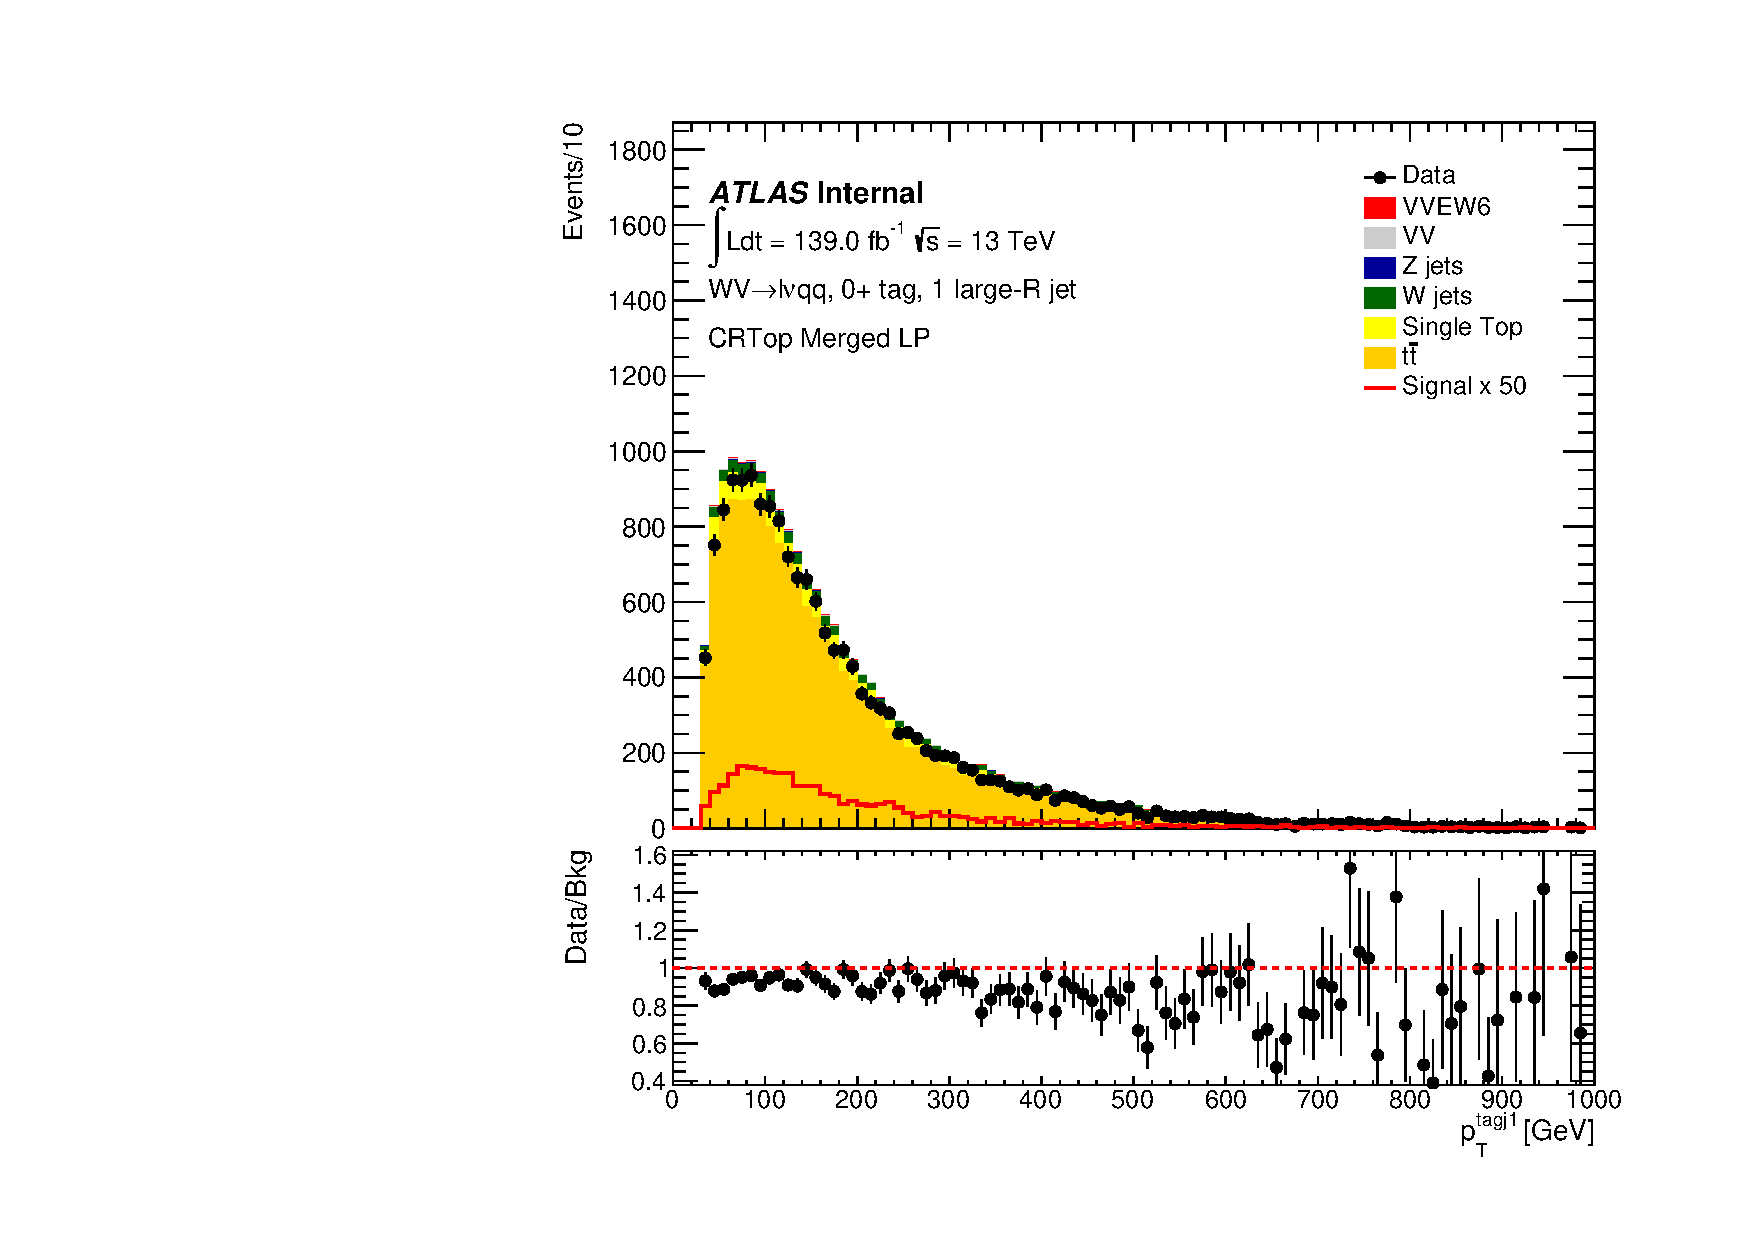
\includegraphics[width=0.3\textwidth]{figures/CRPlots/CRTop_80/stacked_plot_merged_tagJ1_pt.pdf}}
    \subfloat[]{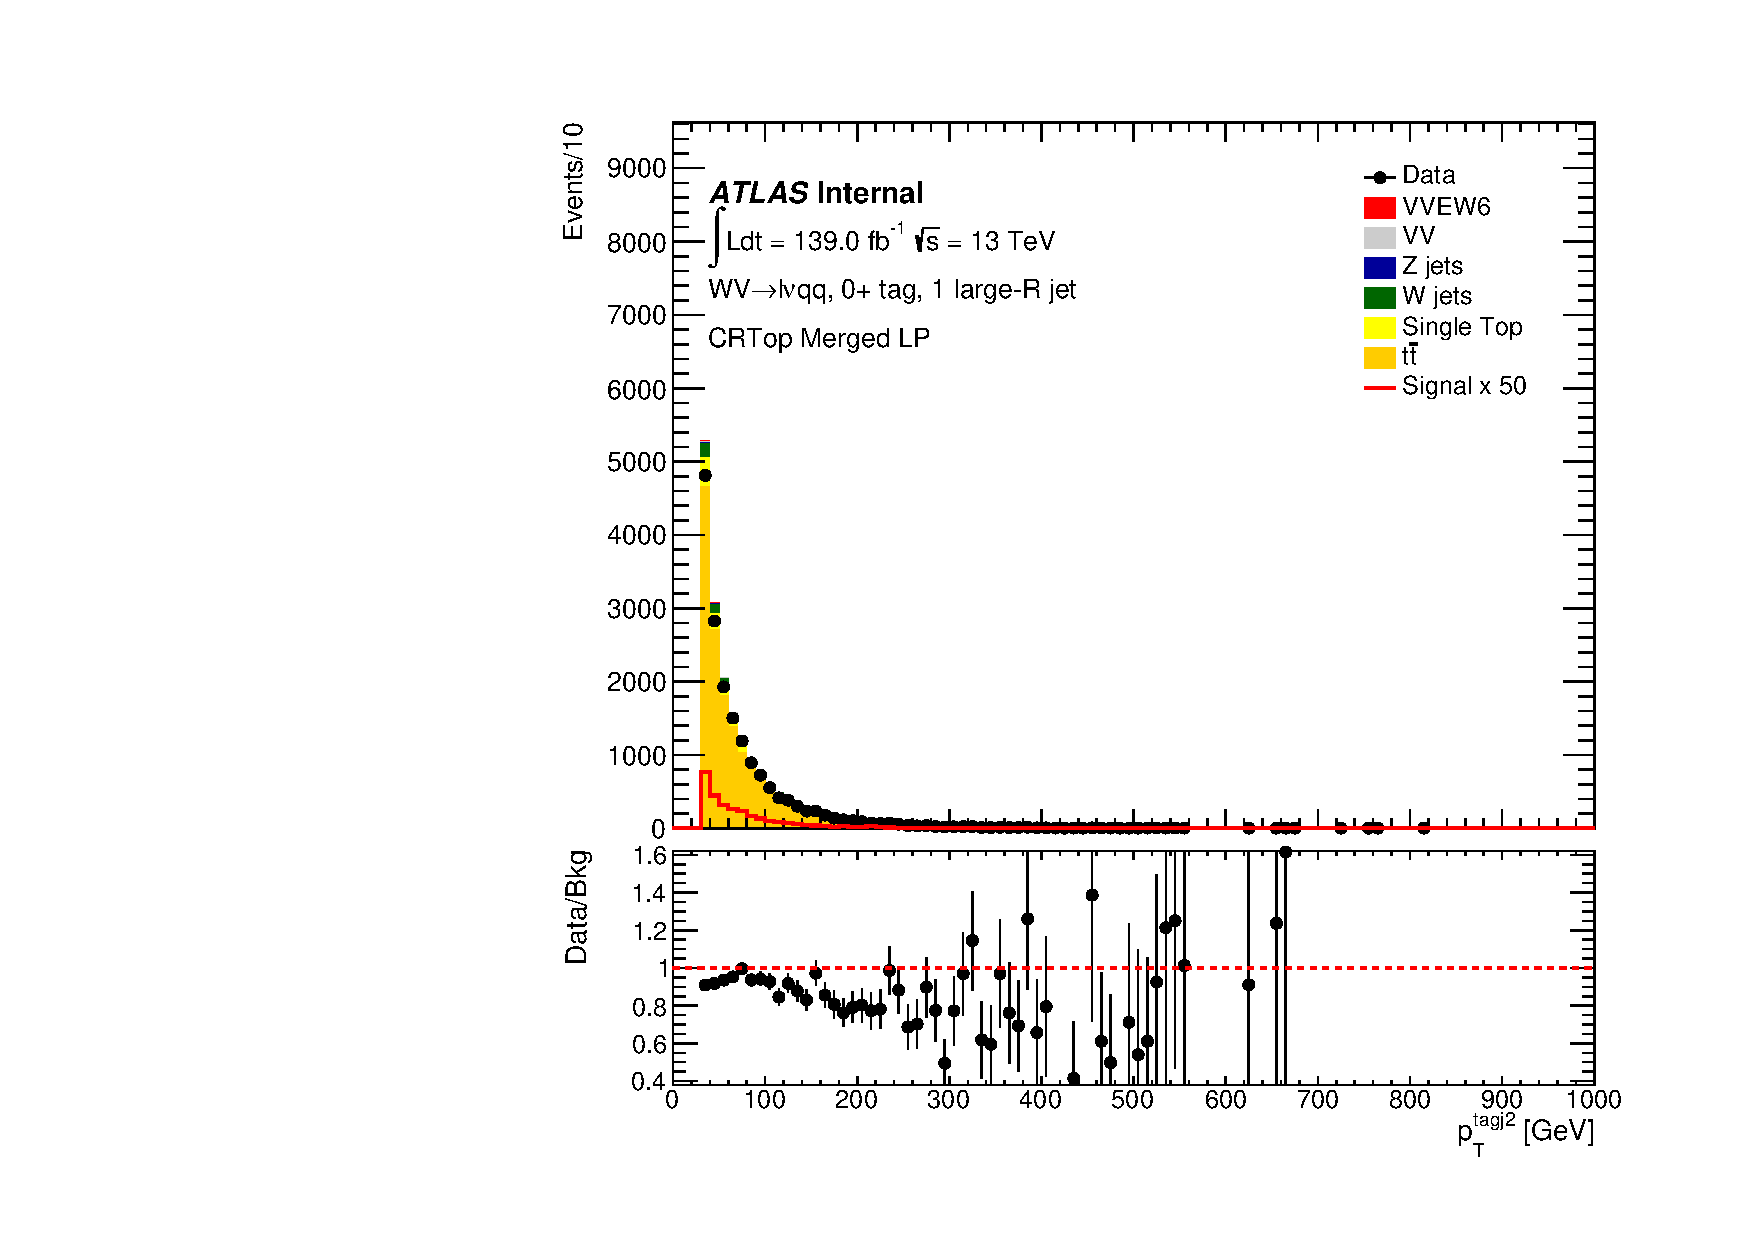
\includegraphics[width=0.3\textwidth]{figures/CRPlots/CRTop_80/stacked_plot_merged_tagJ2_pt.pdf}} \\
    \subfloat[]{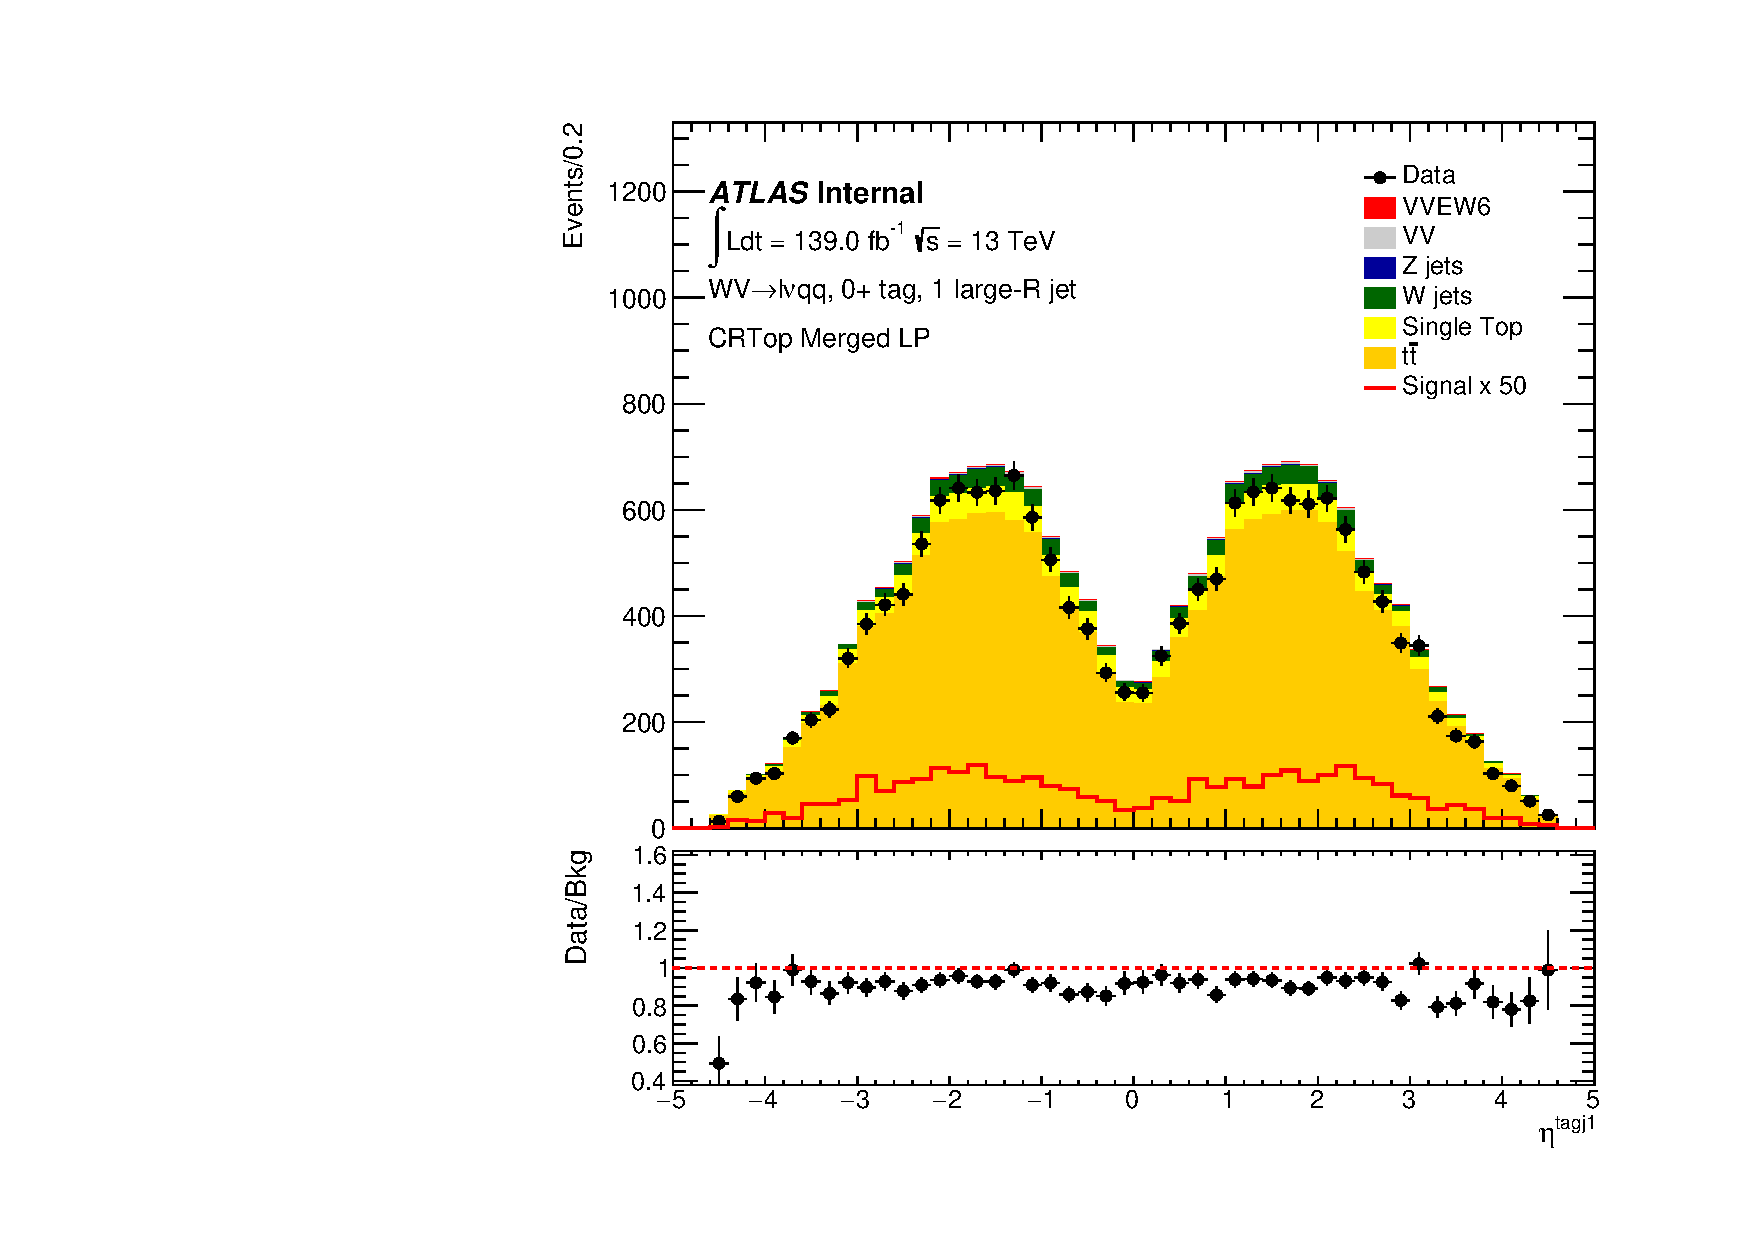
\includegraphics[width=0.3\textwidth]{figures/CRPlots/CRTop_80/stacked_plot_merged_tagJ1_eta.pdf}}
    \subfloat[]{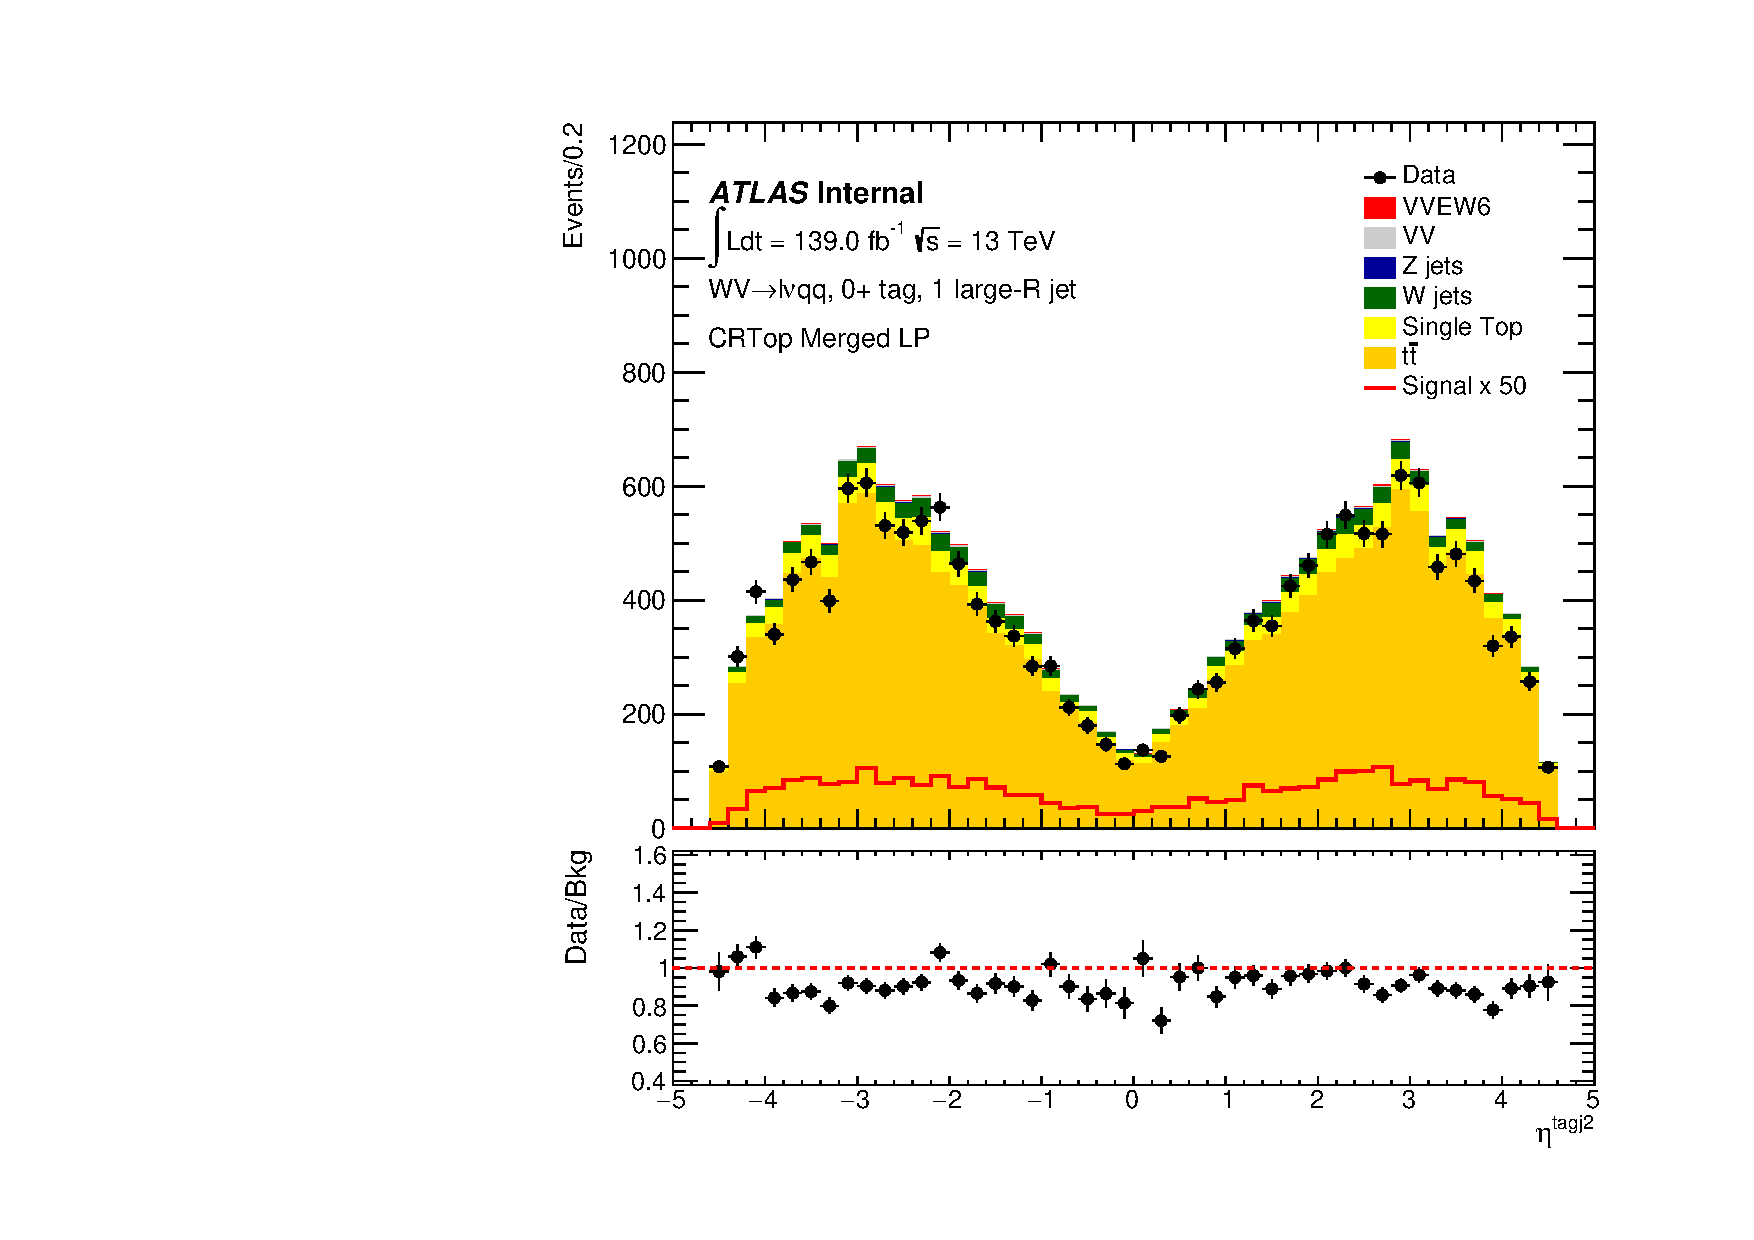
\includegraphics[width=0.3\textwidth]{figures/CRPlots/CRTop_80/stacked_plot_merged_tagJ2_eta.pdf}} \\
    \subfloat[]{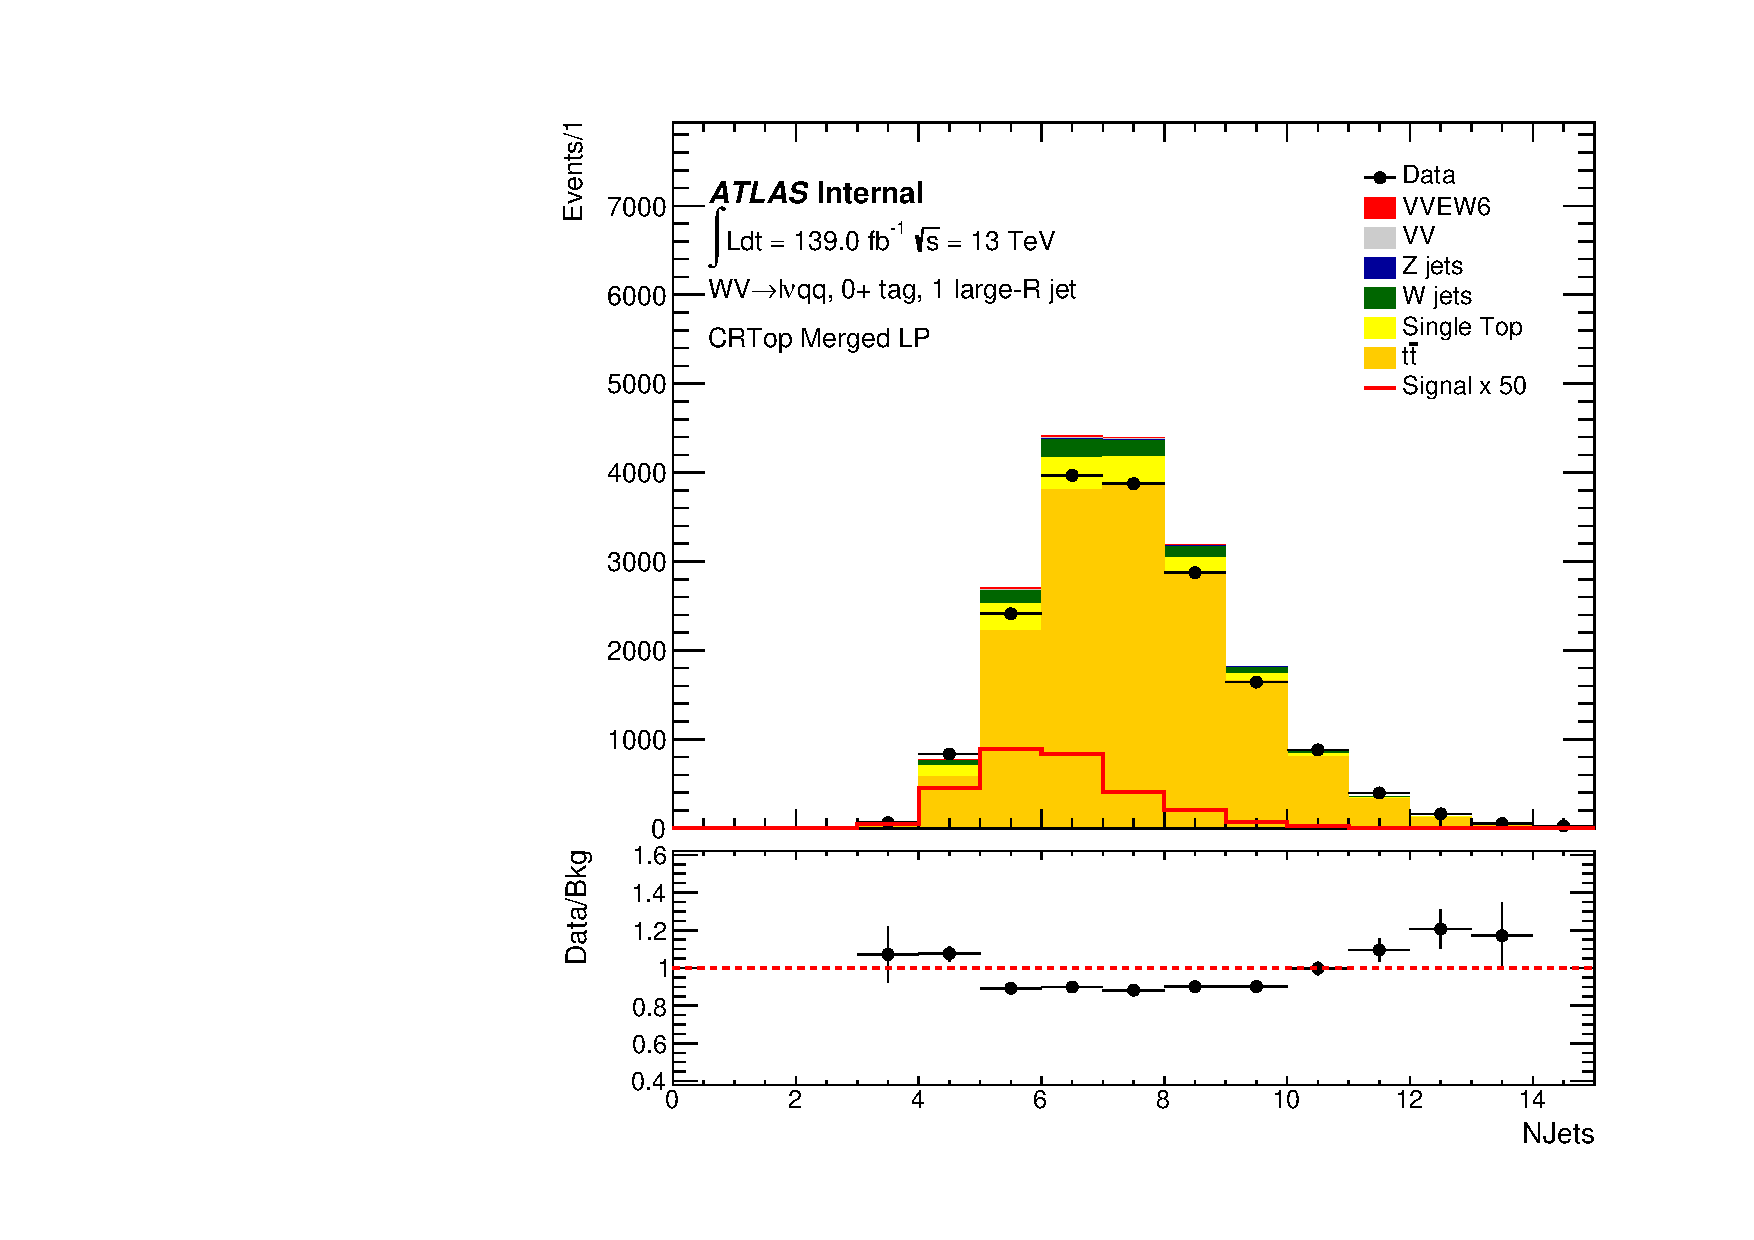
\includegraphics[width=0.3\textwidth]{figures/CRPlots/CRTop_80/stacked_plot_NJets.pdf}}
    \subfloat[]{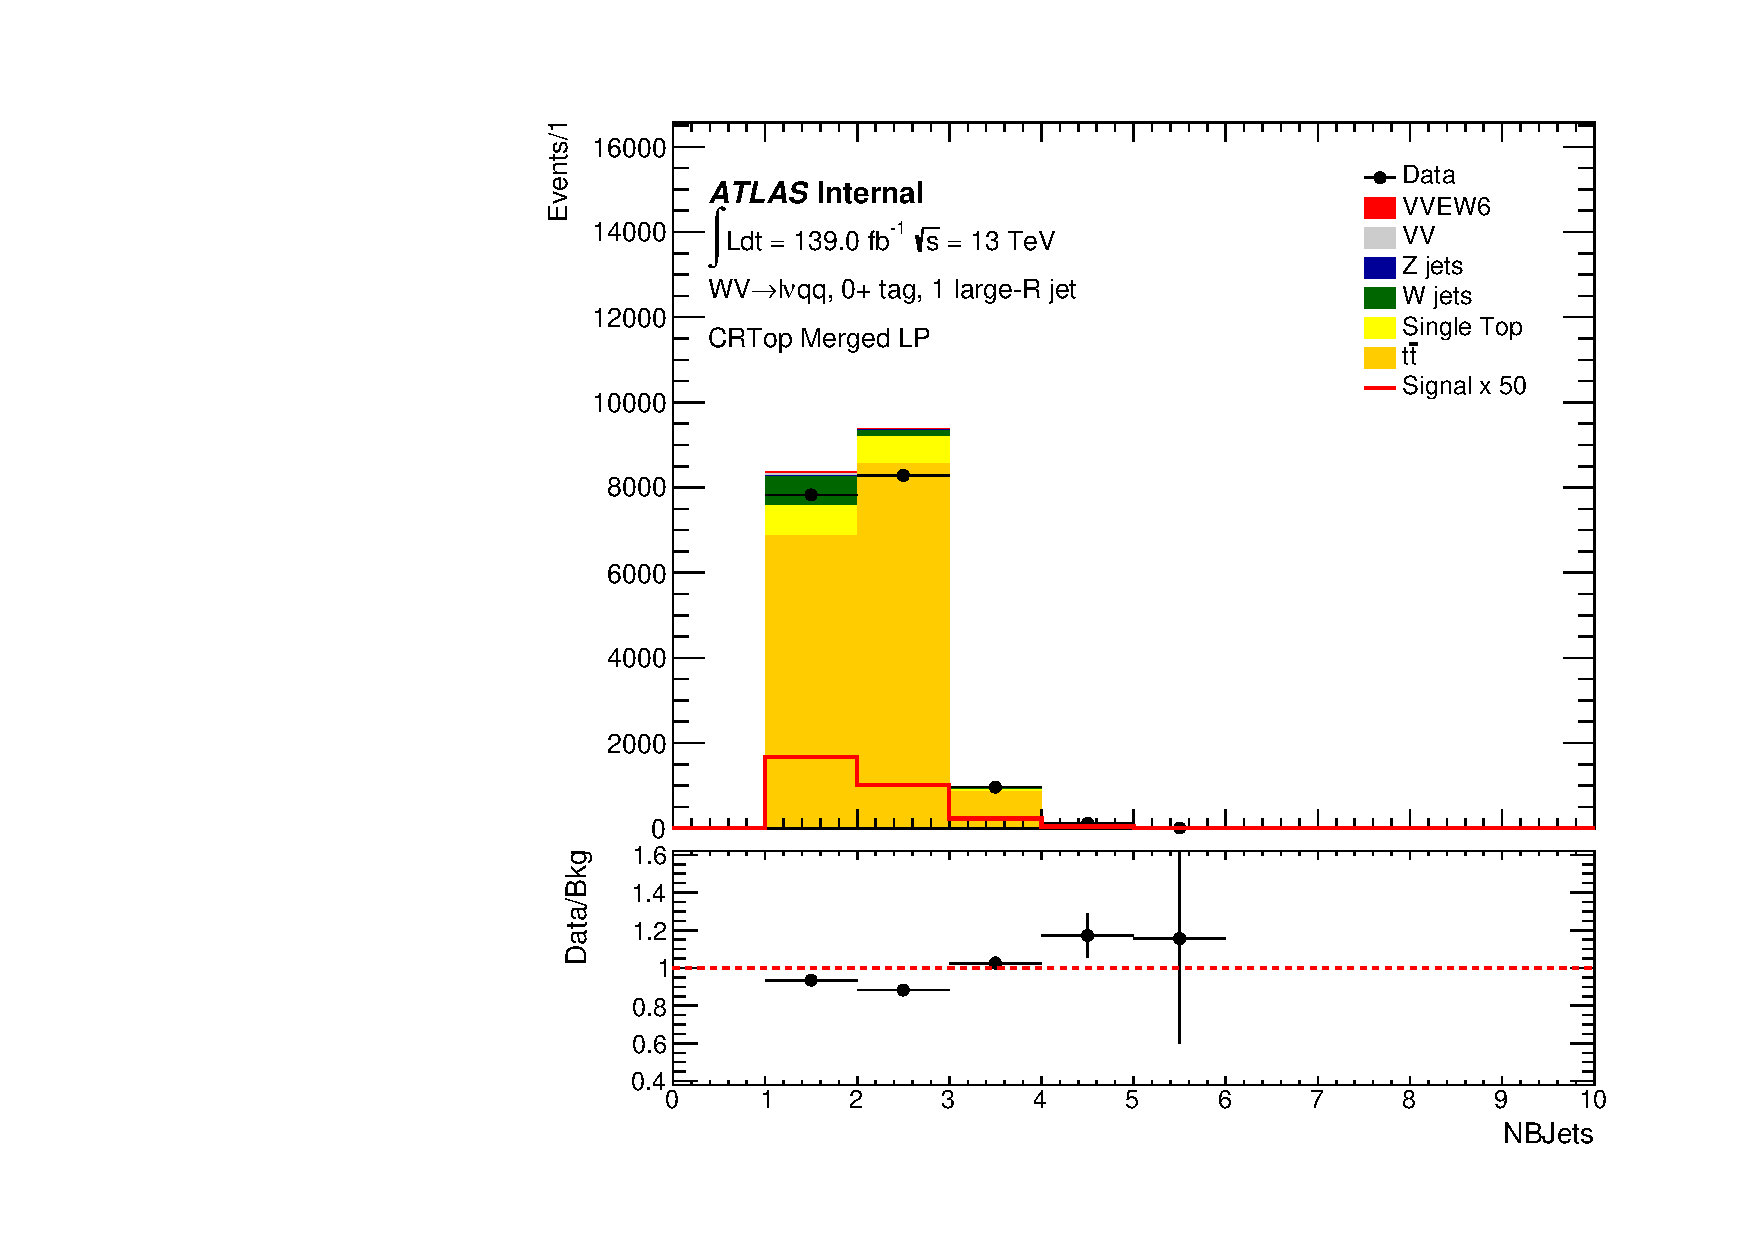
\includegraphics[width=0.3\textwidth]{figures/CRPlots/CRTop_80/stacked_plot_NBJets.pdf}}
    \subfloat[]{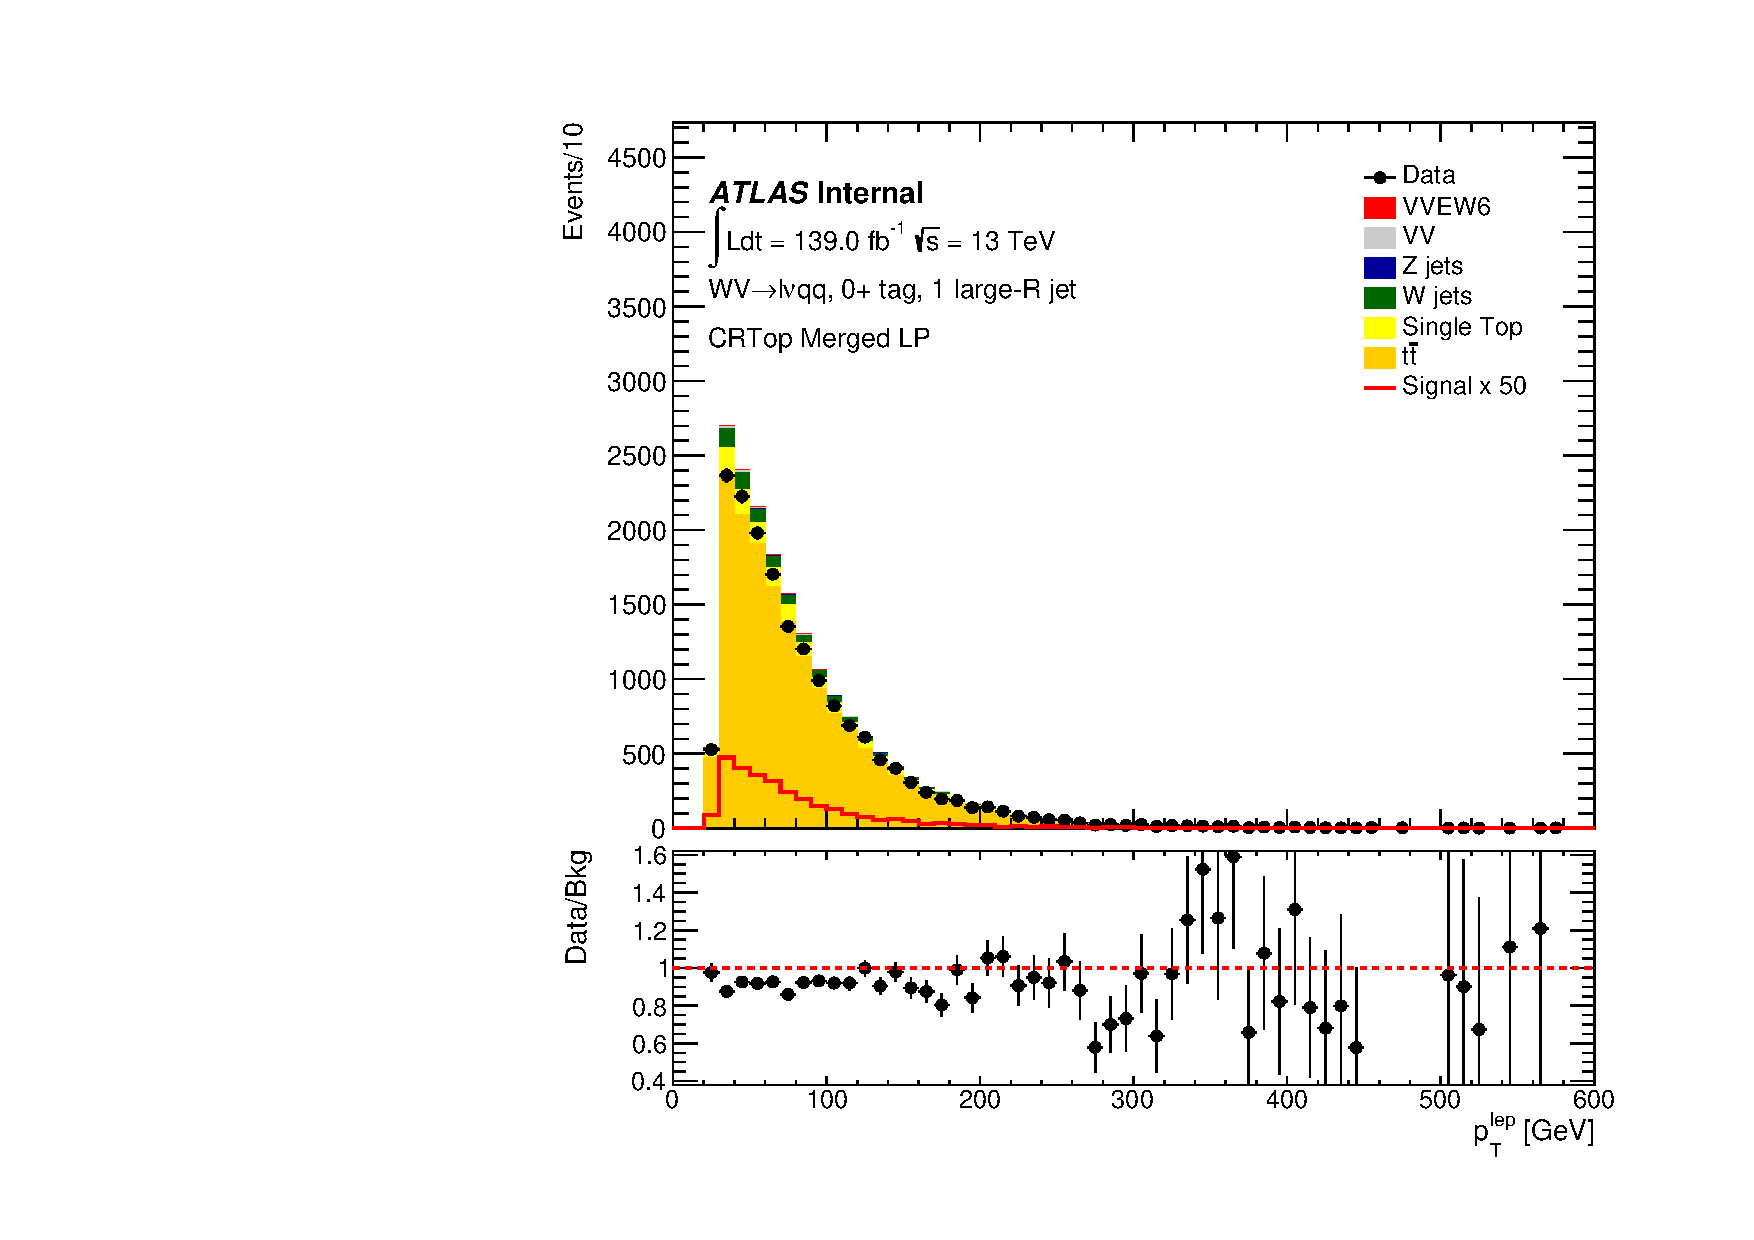
\includegraphics[width=0.3\textwidth]{figures/CRPlots/CRTop_80/stacked_plot_lep_pt.pdf}} \\
    \subfloat[]{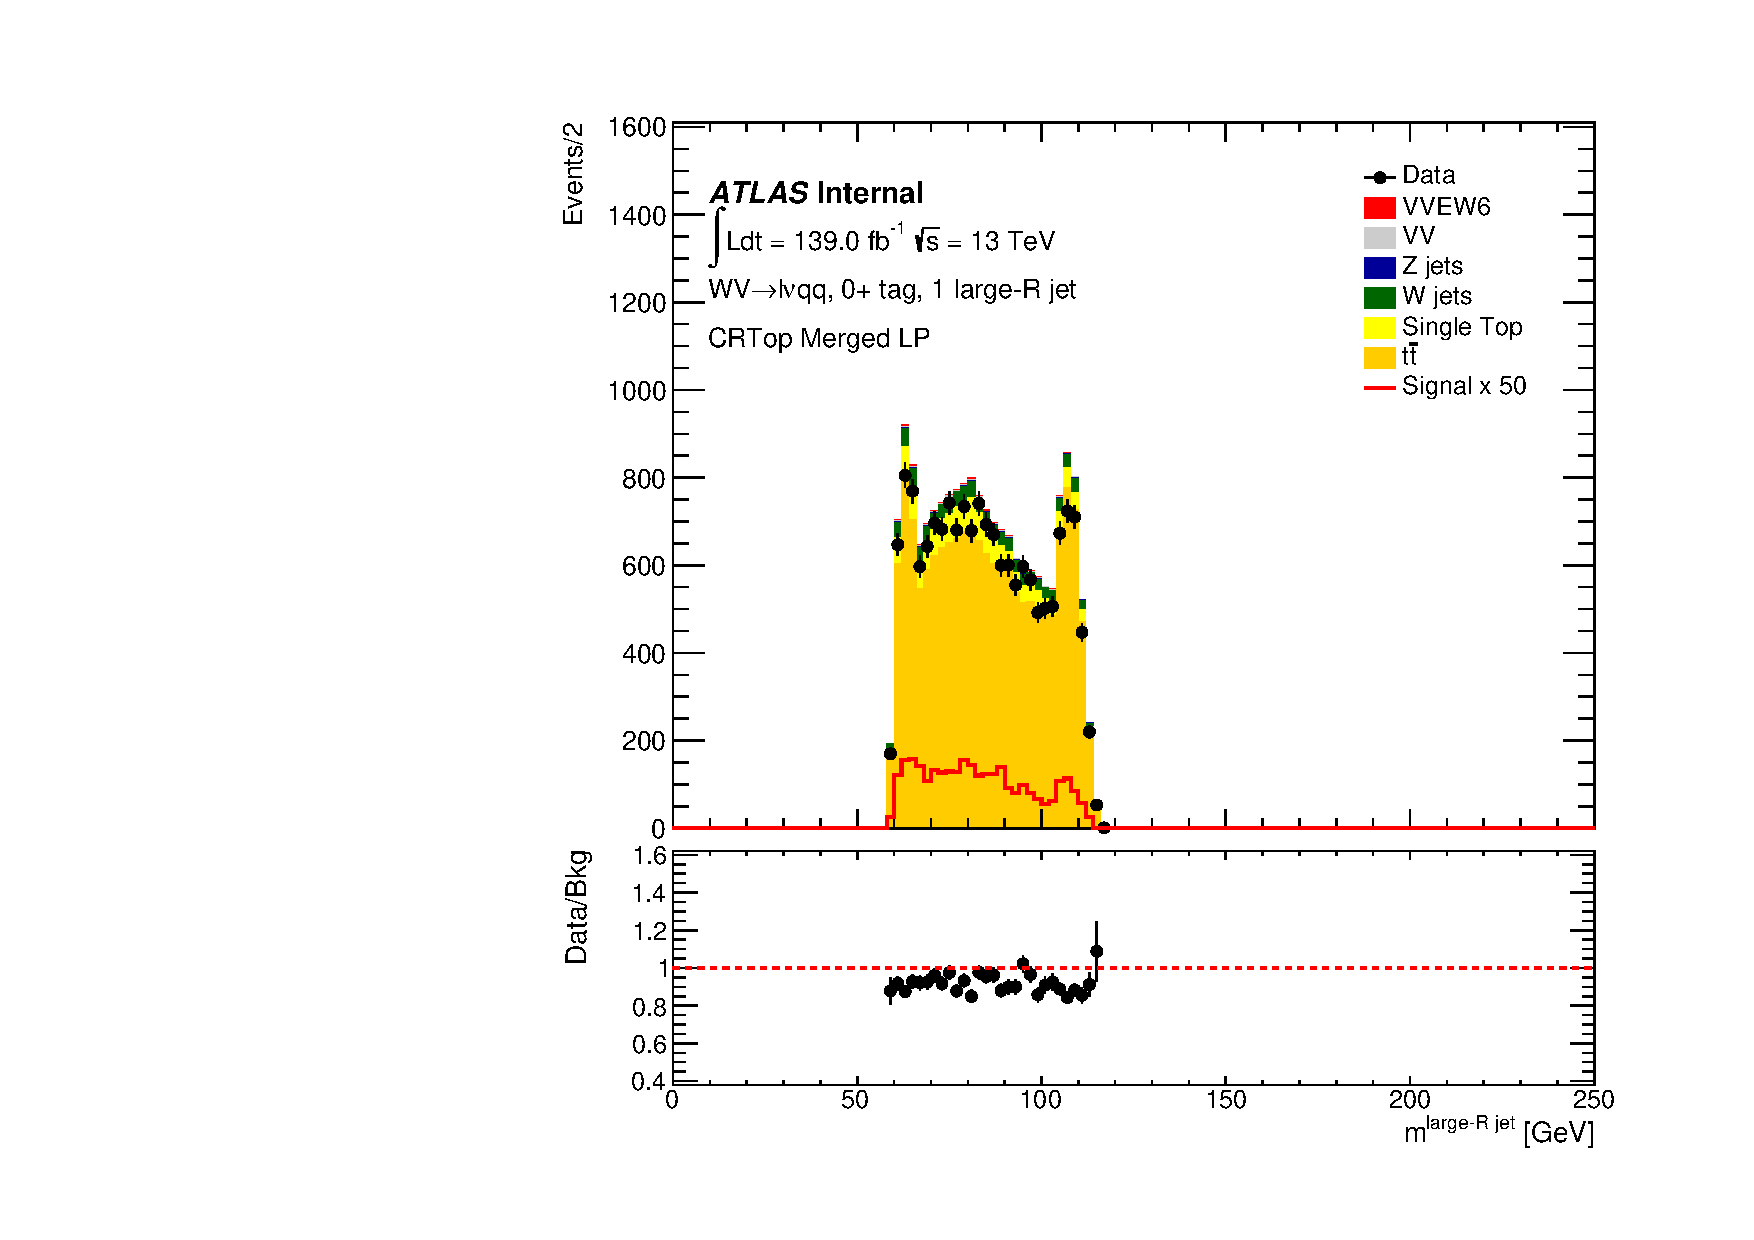
\includegraphics[width=0.3\textwidth]{figures/CRPlots/CRTop_80/stacked_plot_fatJ_m.pdf}}
    \subfloat[]{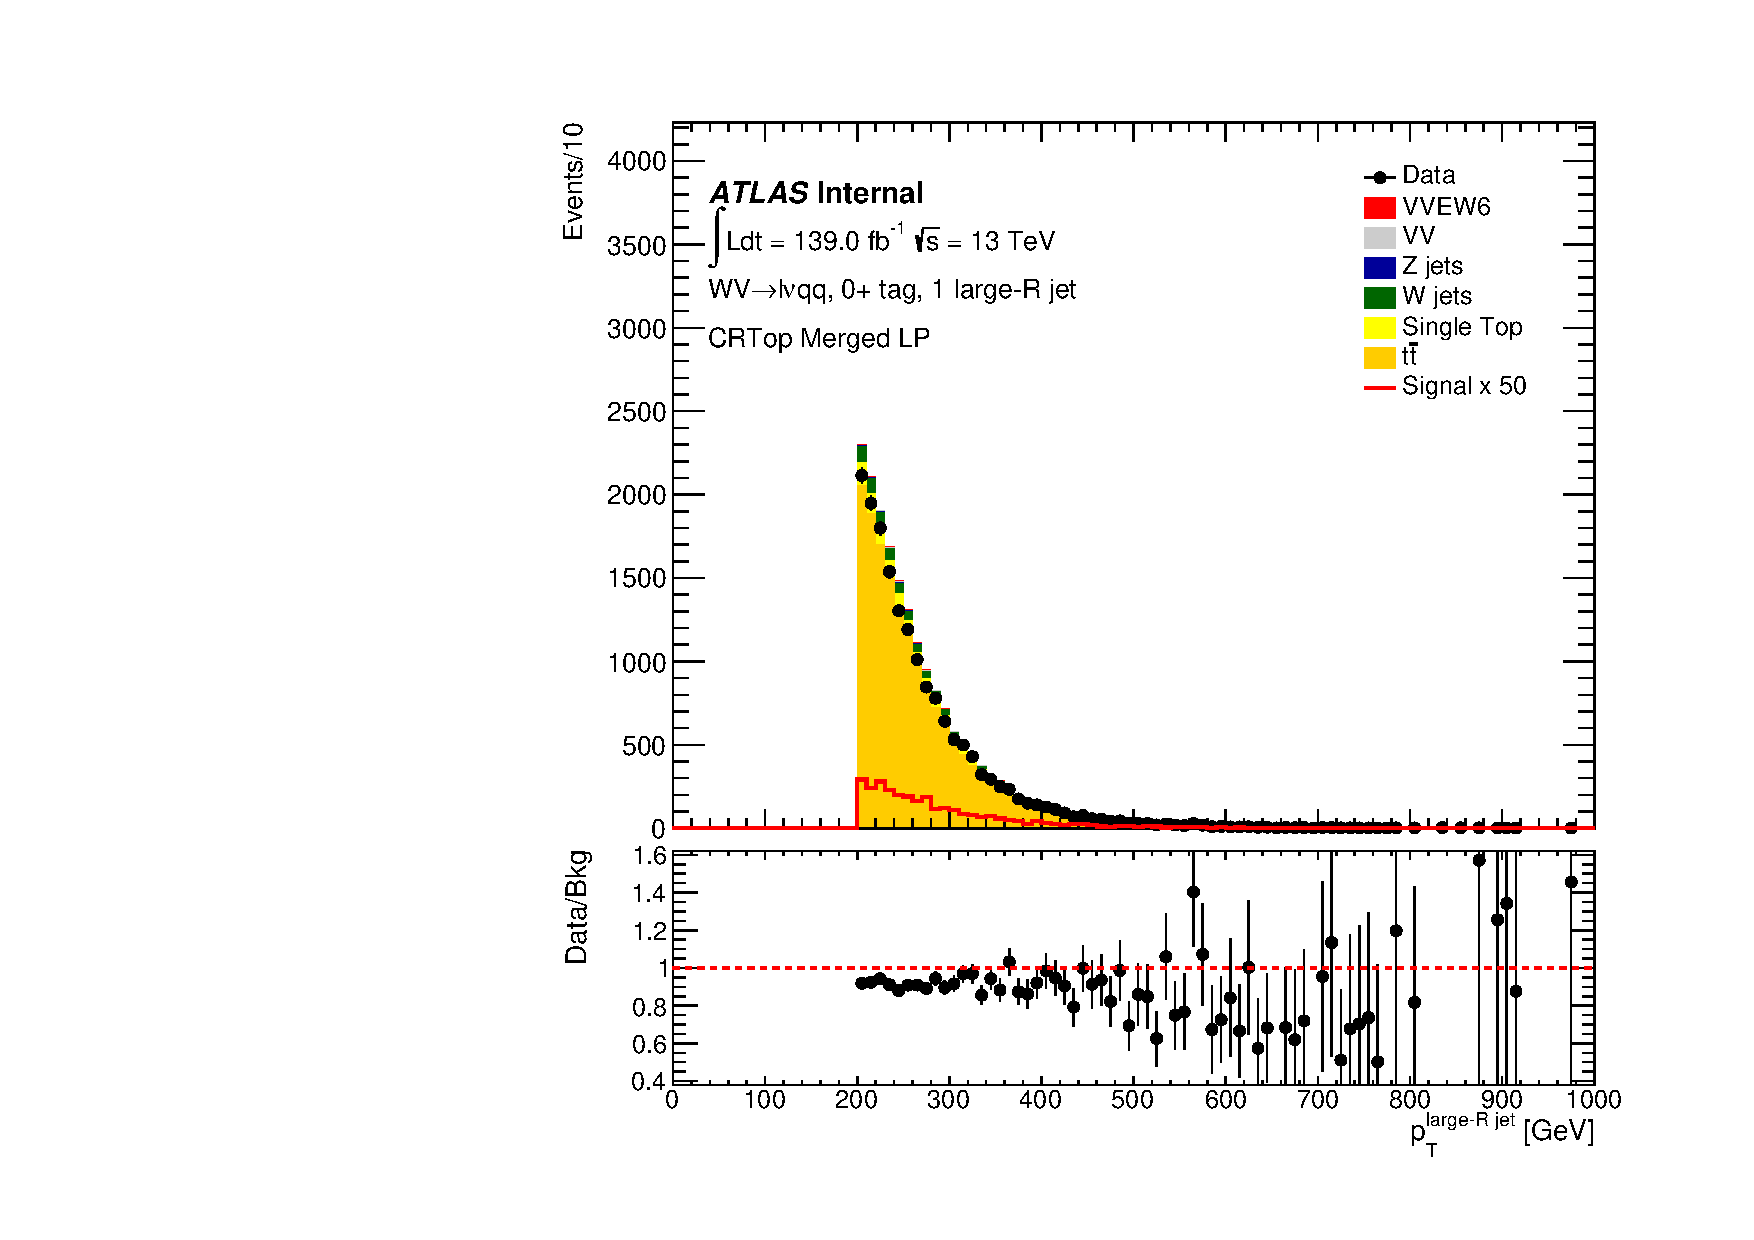
\includegraphics[width=0.3\textwidth]{figures/CRPlots/CRTop_80/stacked_plot_fatJ_pt.pdf}}
    \subfloat[]{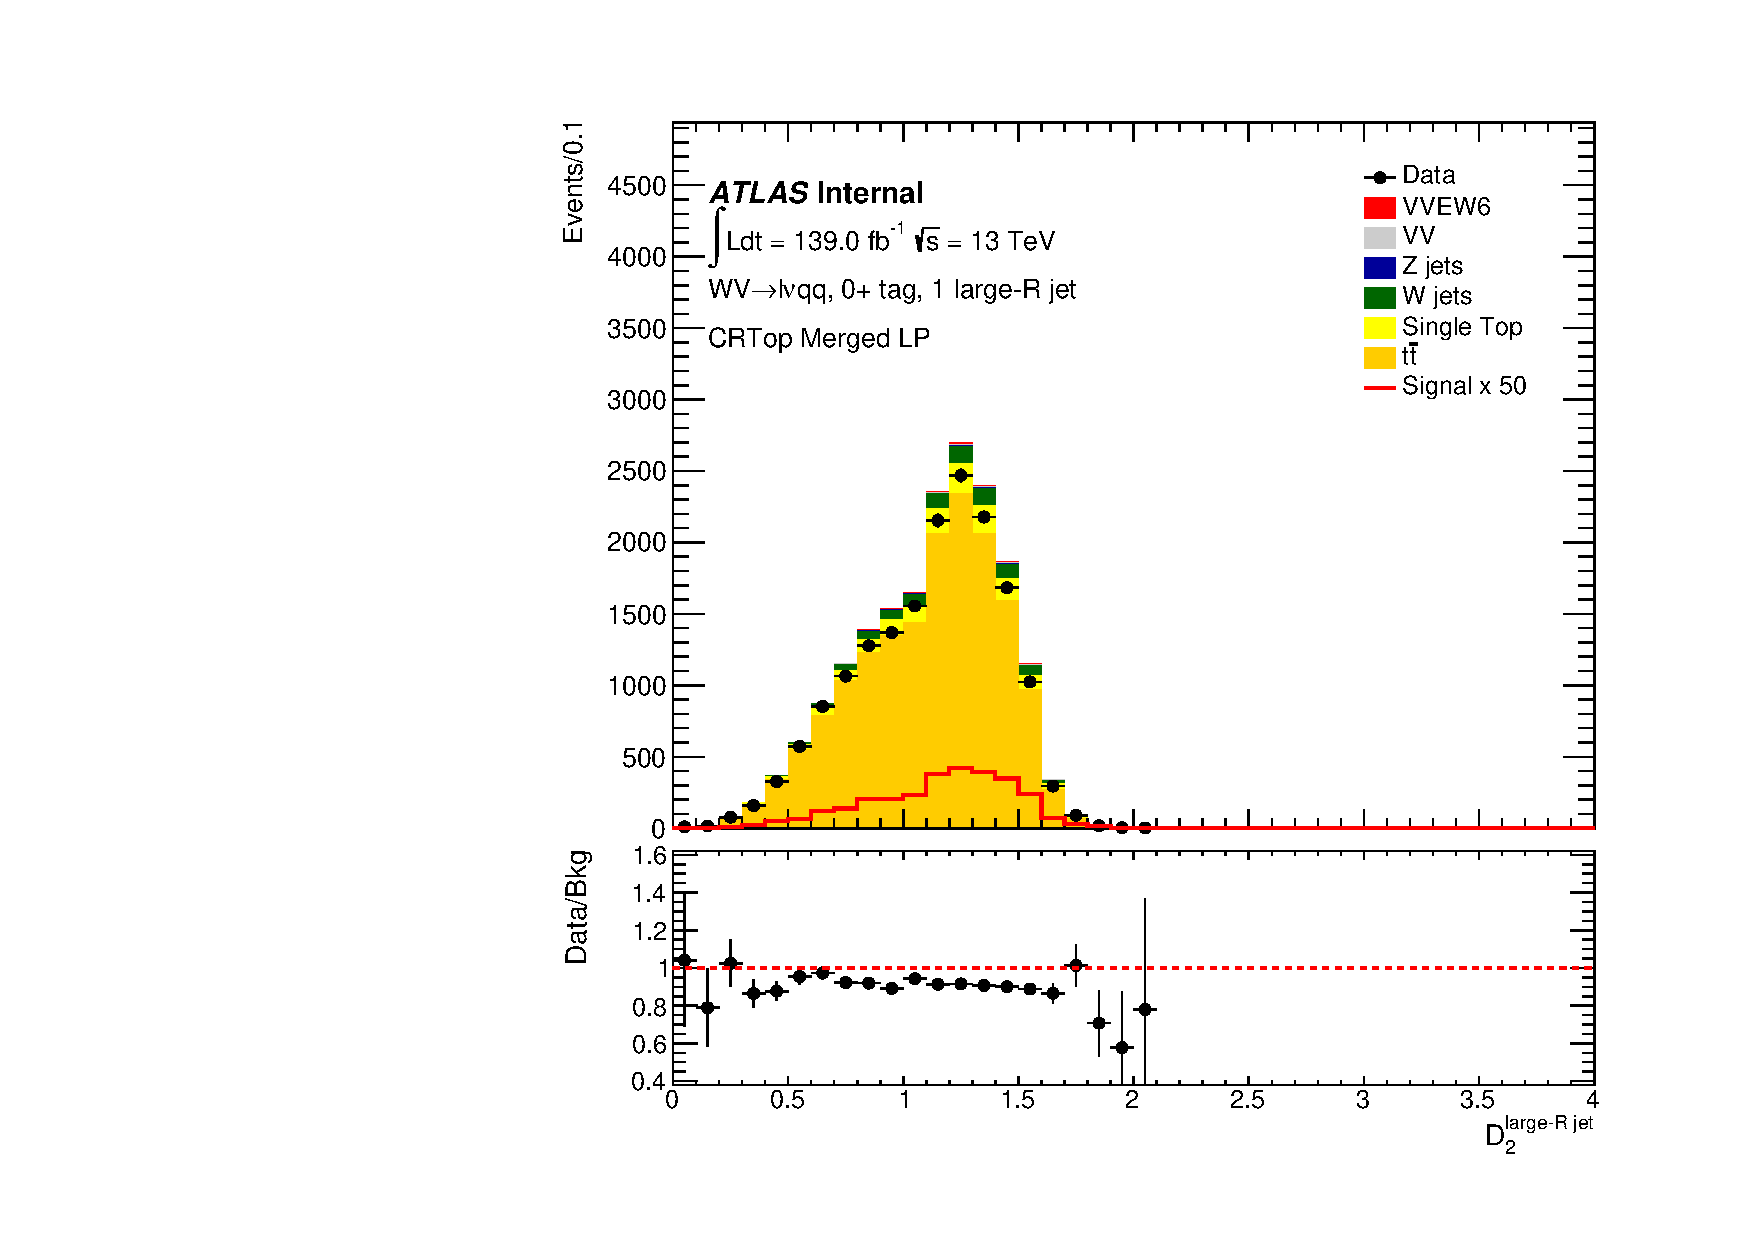
\includegraphics[width=0.3\textwidth]{figures/CRPlots/CRTop_80/stacked_plot_fatJ_D2.pdf}}
    \caption{Data-MC checks for the merged low-purity top control region in the \olep channel.}
    \label{fig:CRTopMerLPPlots1Lep}
\end{figure}

\begin{figure}[ht]
    \centering
    \subfloat[]{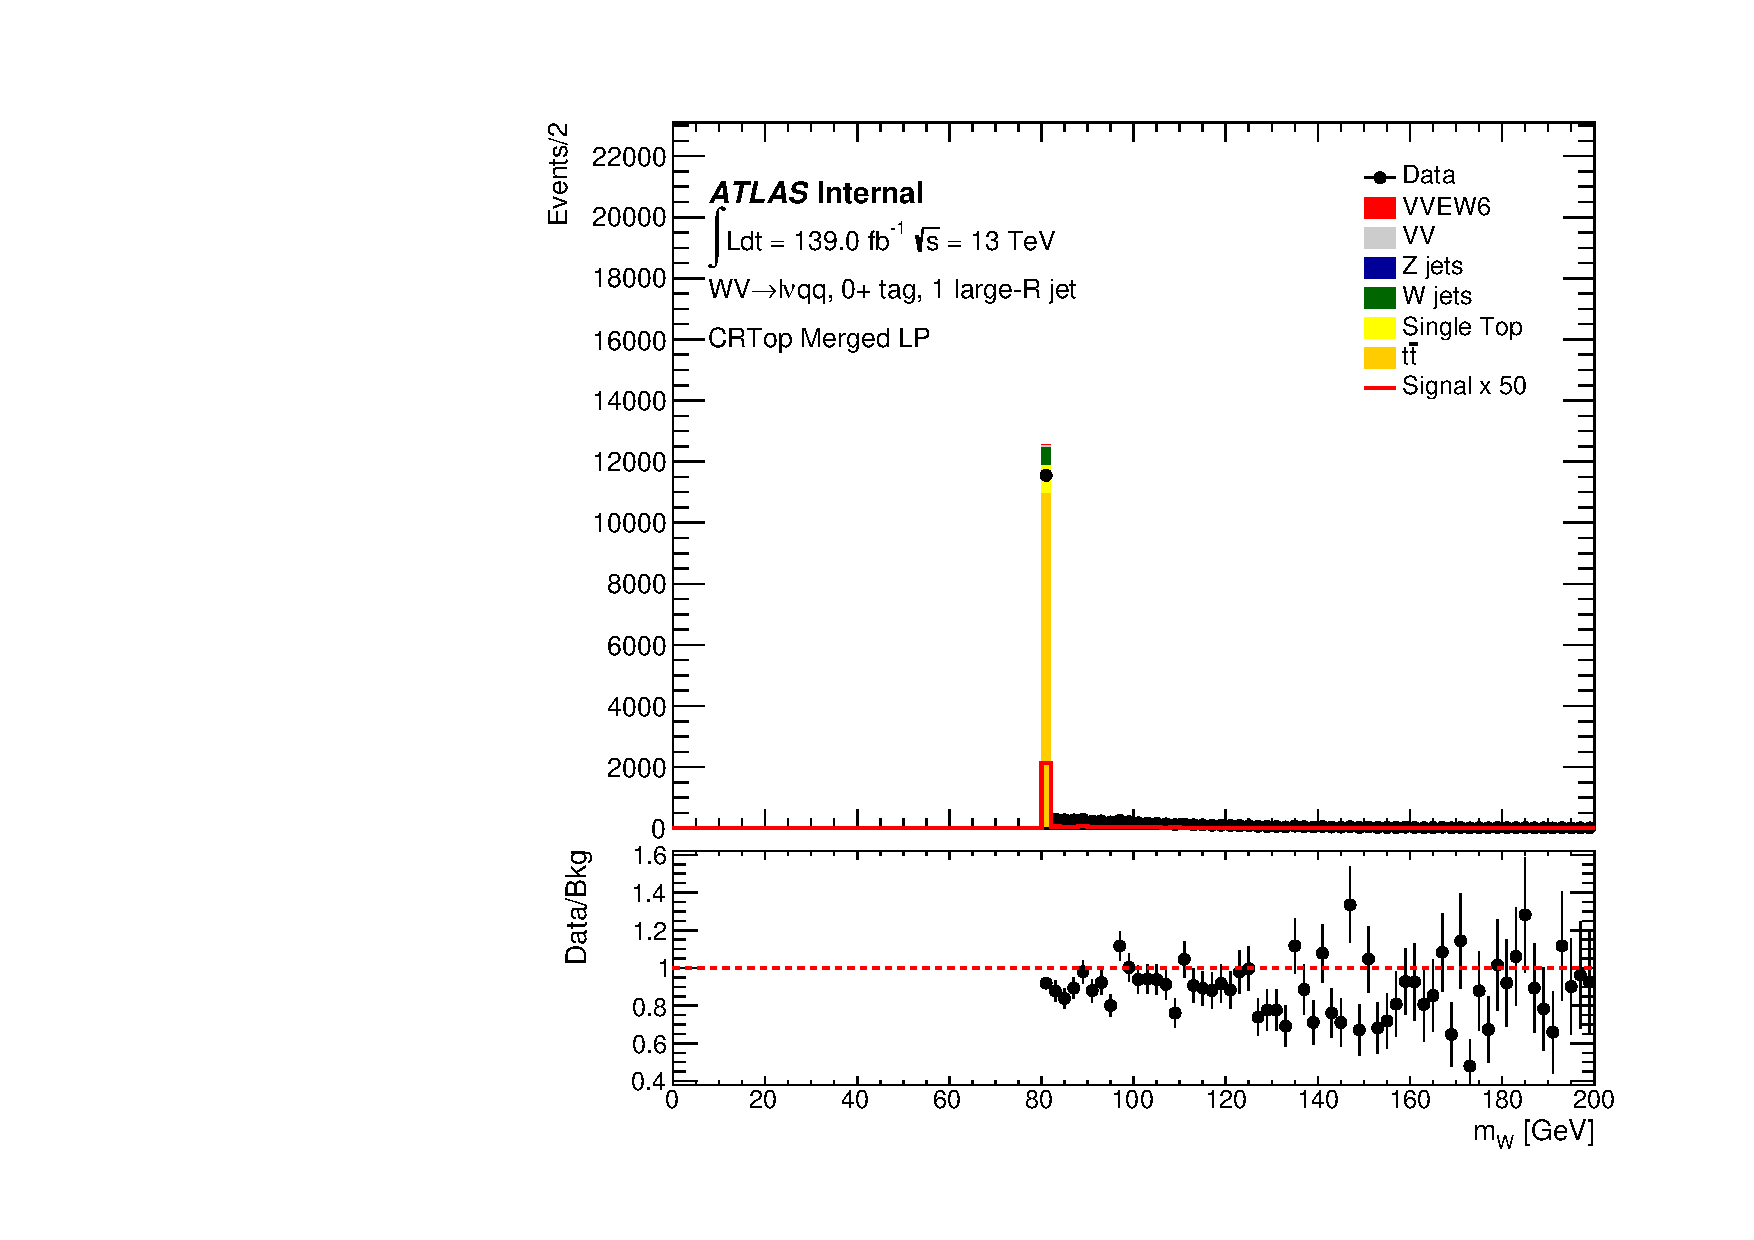
\includegraphics[width=0.3\textwidth]{figures/CRPlots/CRTop_80/stacked_plot_W_m.pdf}}
    \subfloat[]{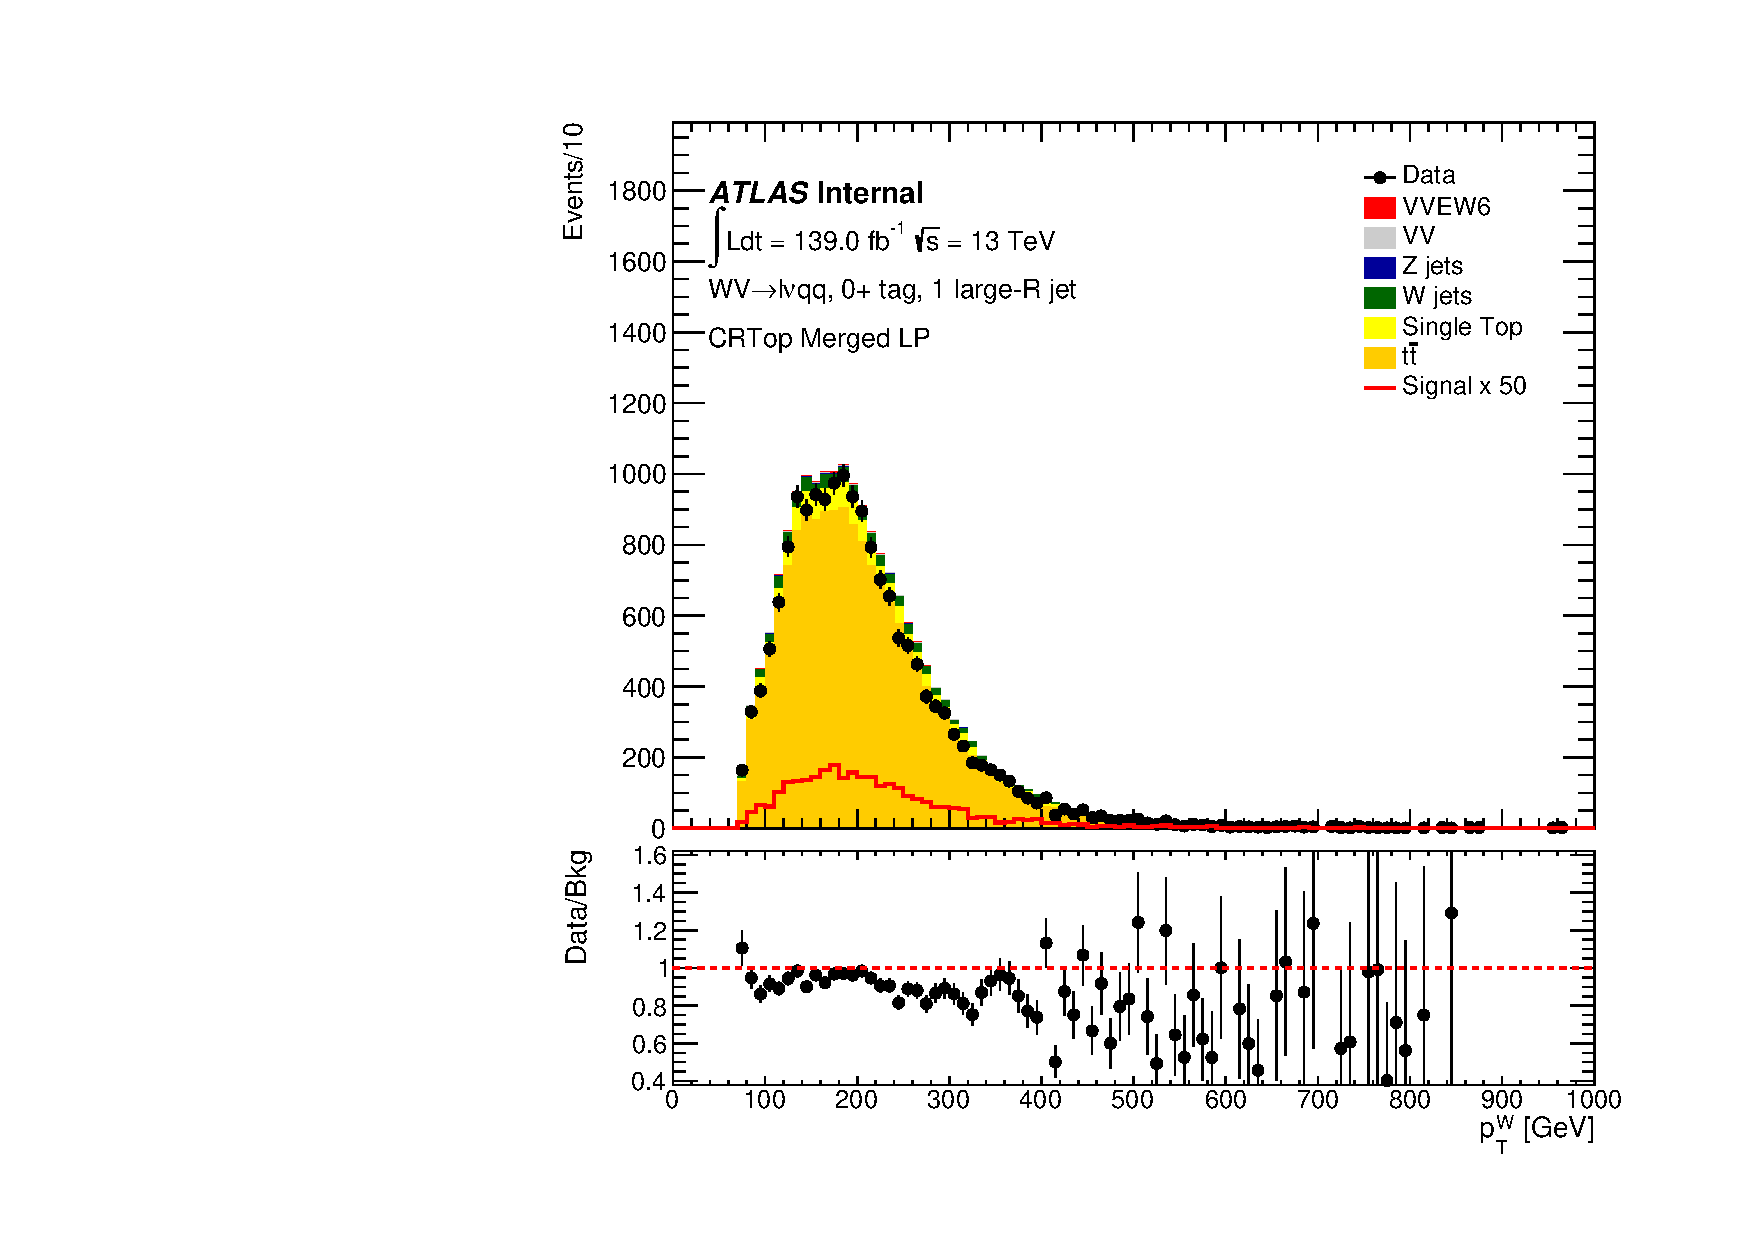
\includegraphics[width=0.3\textwidth]{figures/CRPlots/CRTop_80/stacked_plot_W_pt.pdf}}
    \subfloat[]{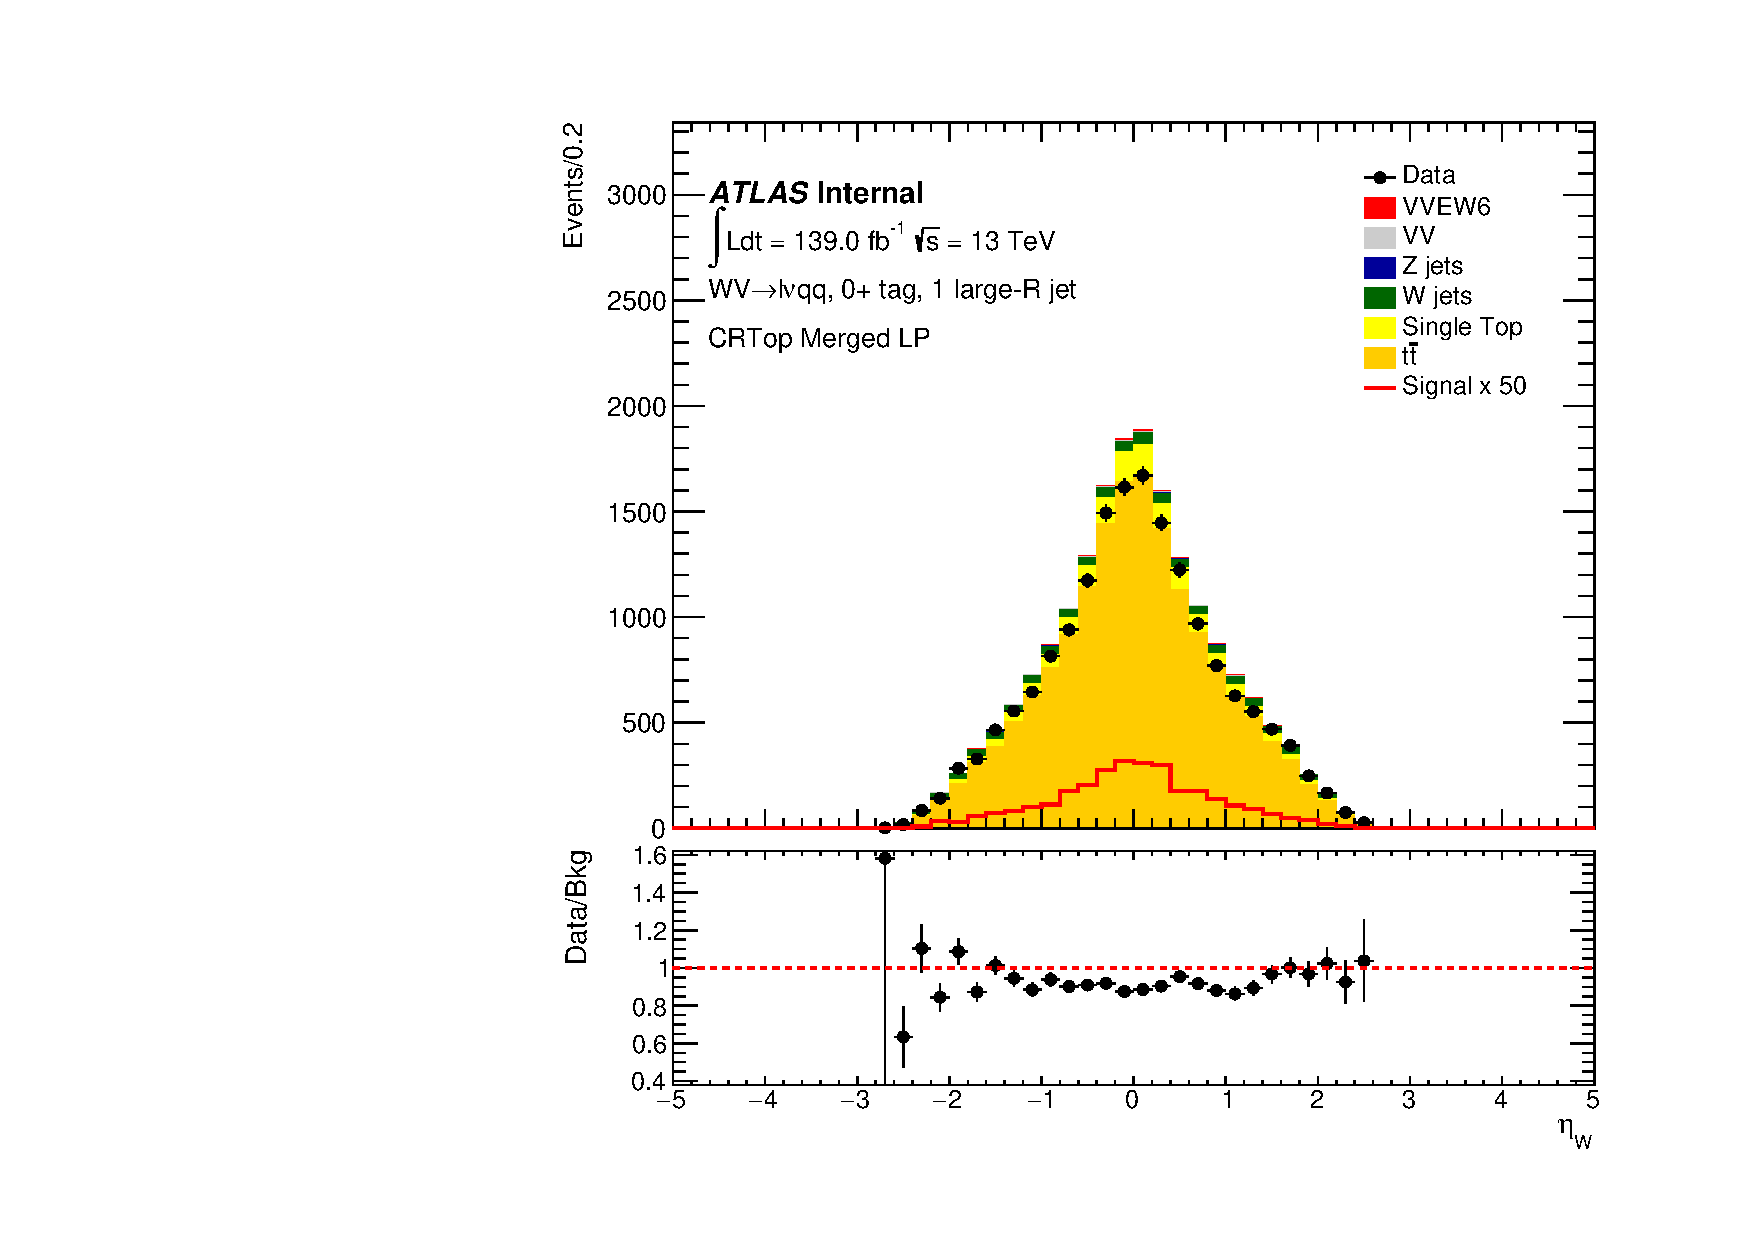
\includegraphics[width=0.3\textwidth]{figures/CRPlots/CRTop_80/stacked_plot_W_eta.pdf}} \\
    \subfloat[]{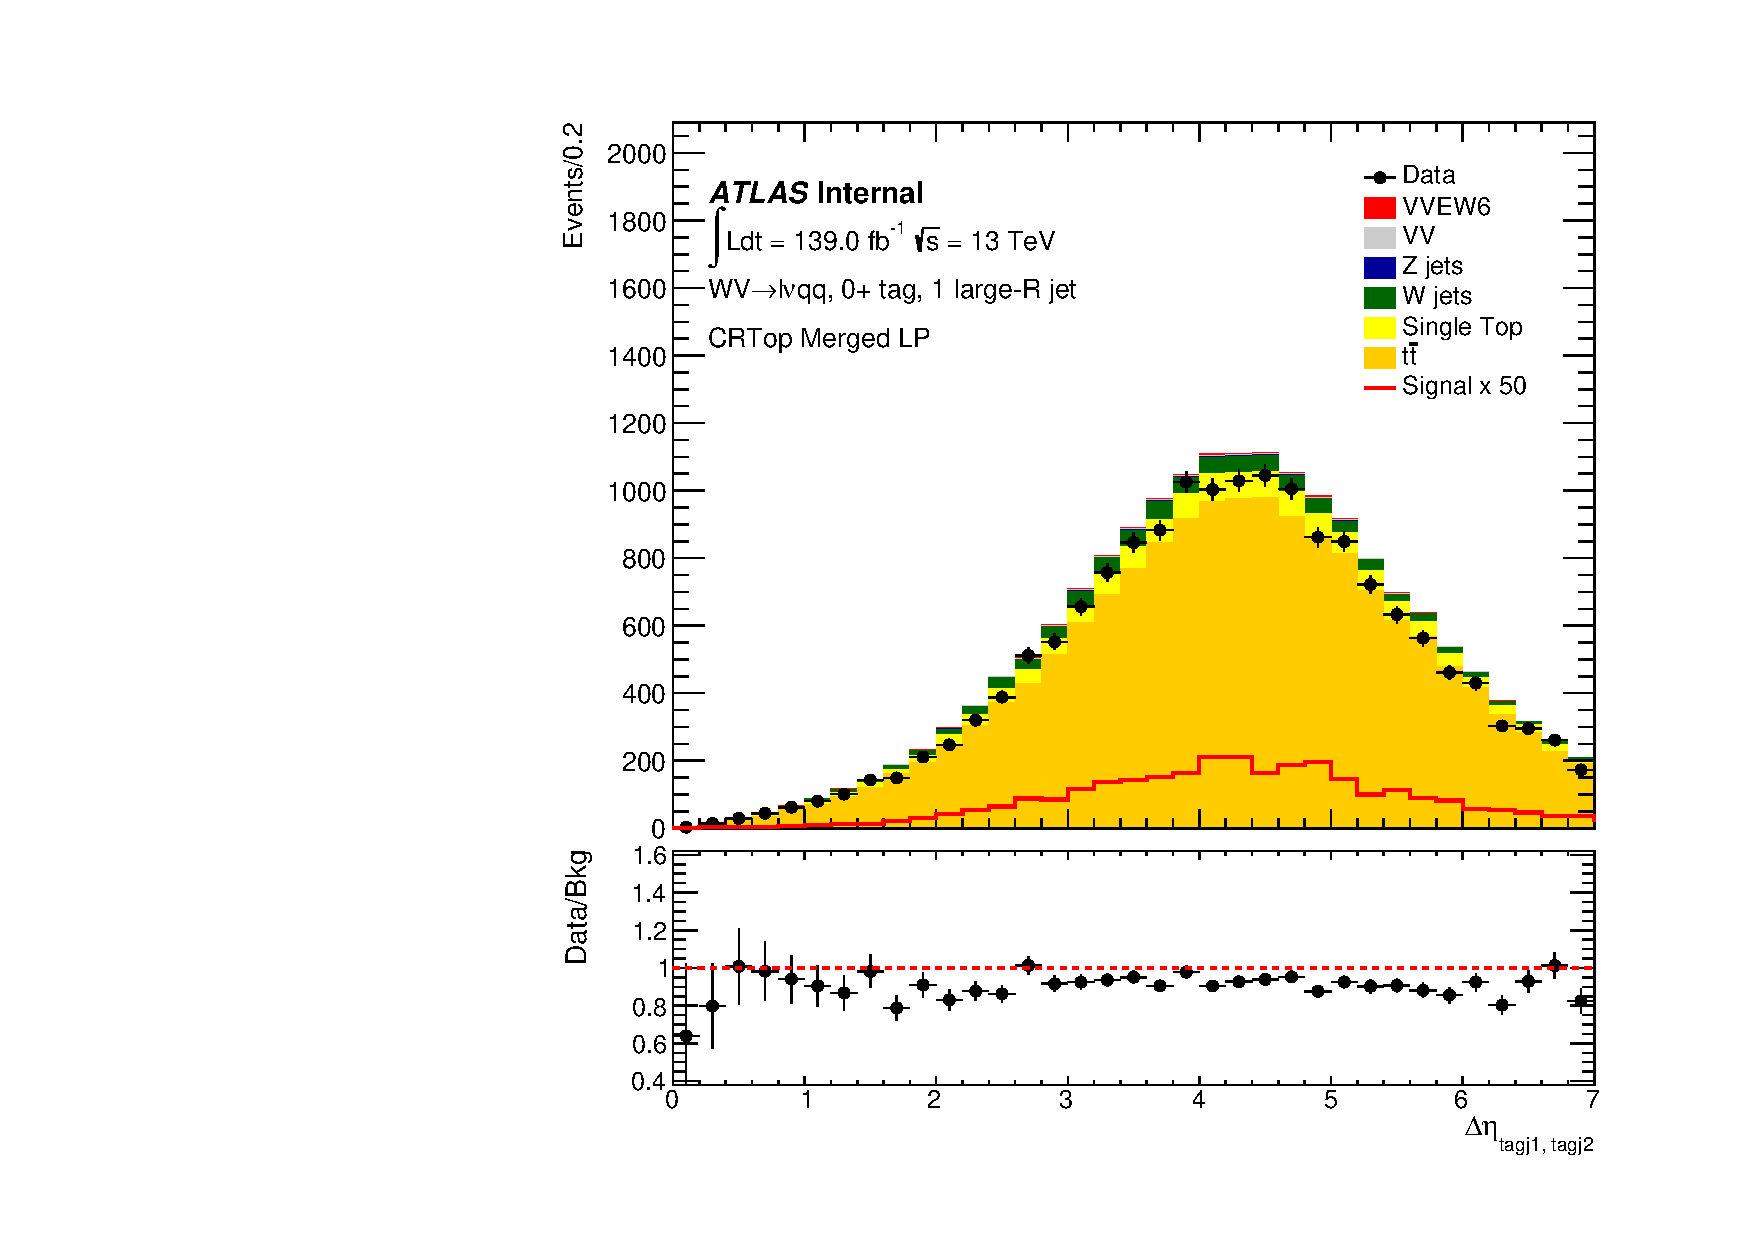
\includegraphics[width=0.3\textwidth]{figures/CRPlots/CRTop_80/stacked_plot_merged_tagJdEta.pdf}}
    \subfloat[]{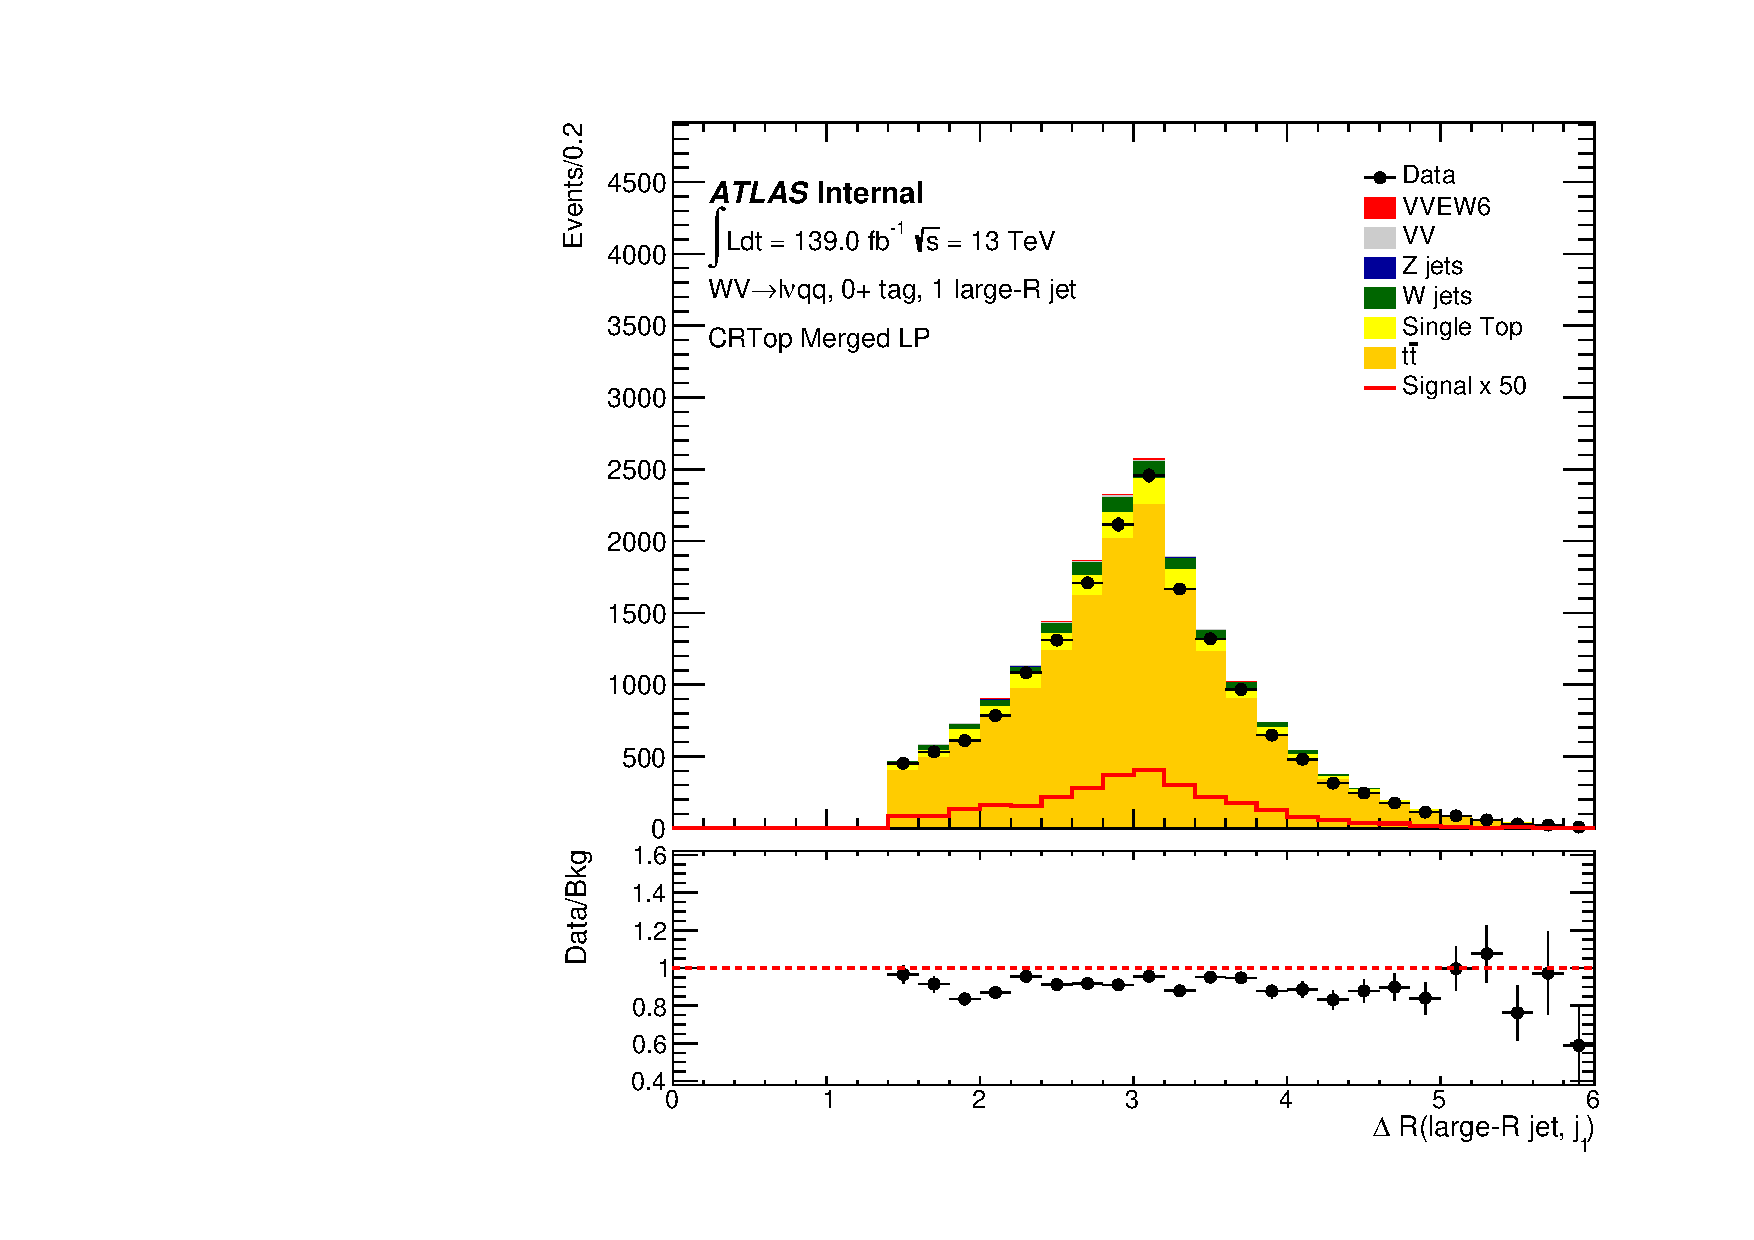
\includegraphics[width=0.3\textwidth]{figures/CRPlots/CRTop_80/stacked_plot_fatJ_dRj1.pdf}}
    \subfloat[]{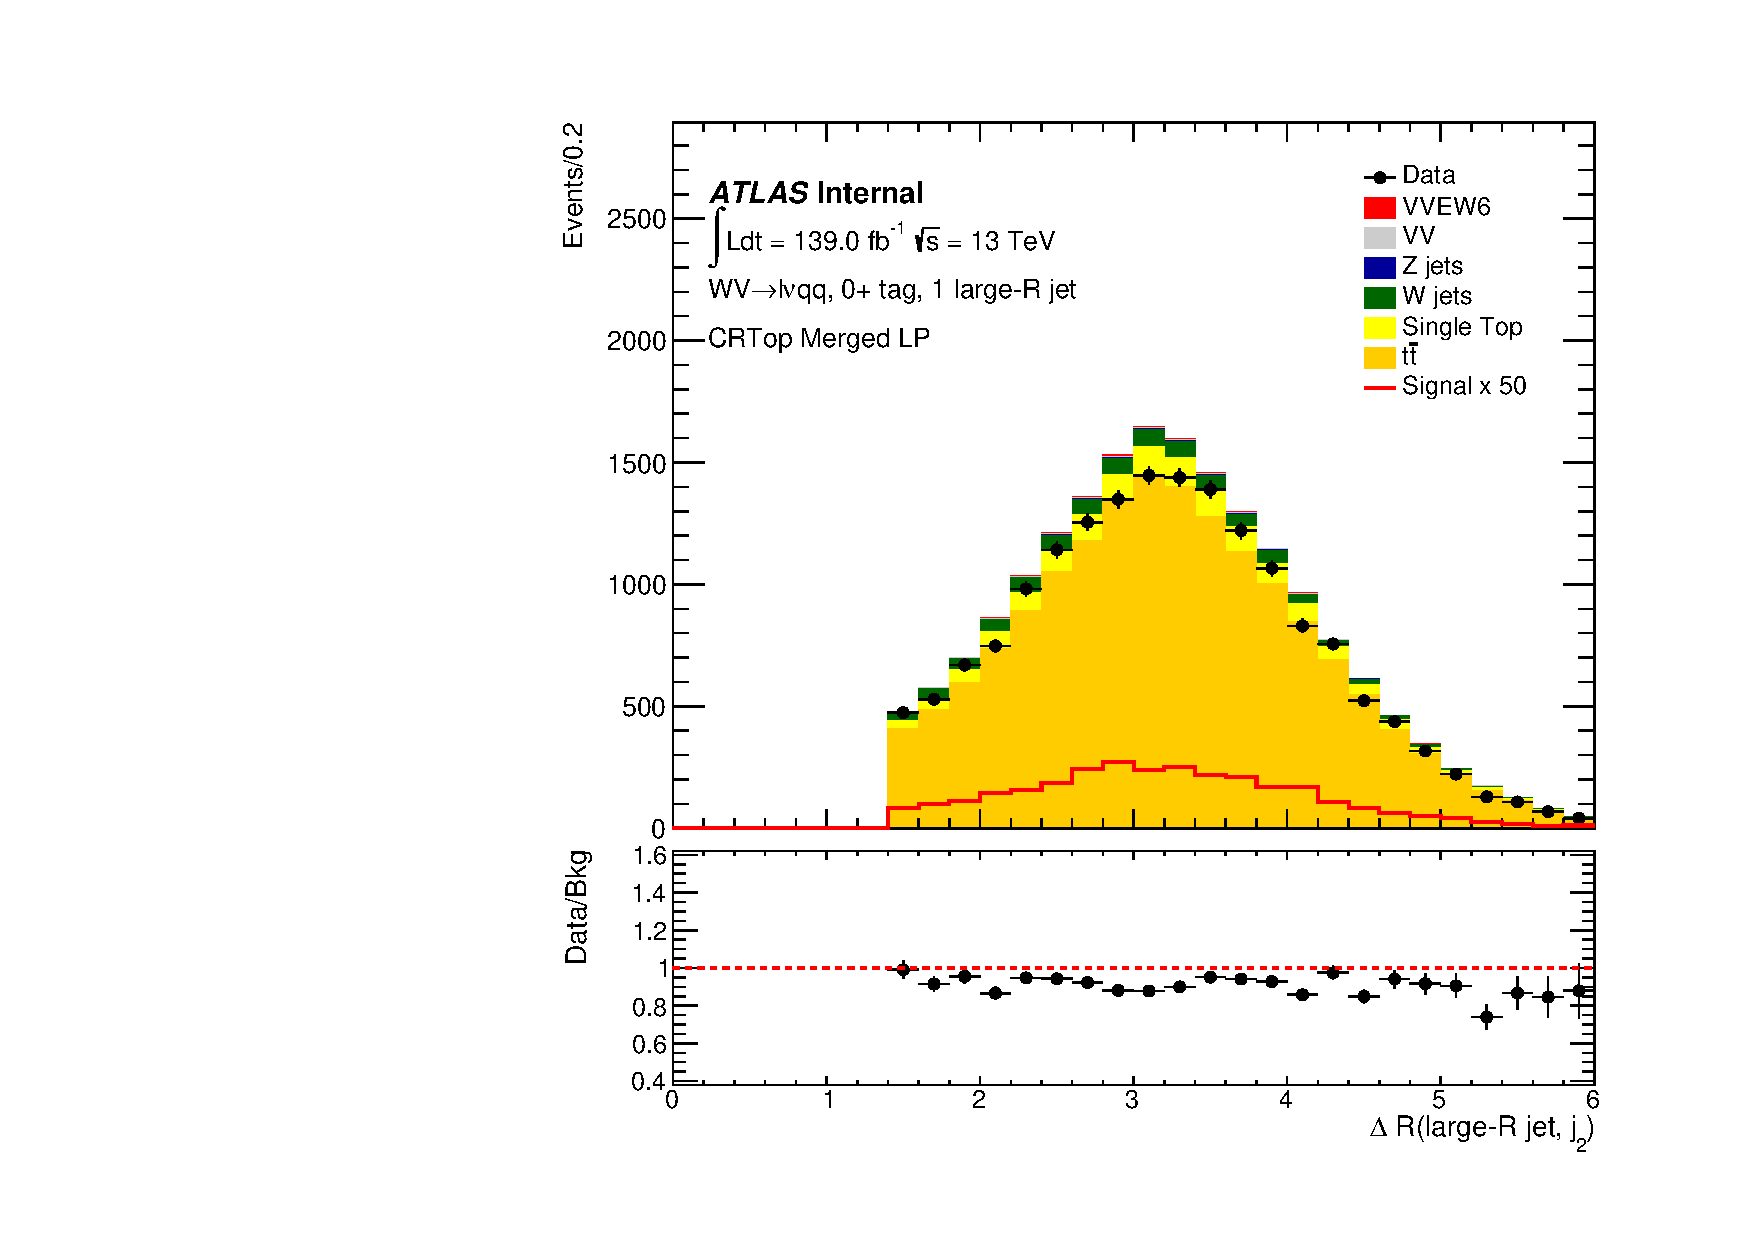
\includegraphics[width=0.3\textwidth]{figures/CRPlots/CRTop_80/stacked_plot_fatJ_dRj2.pdf}} \\
    \subfloat[]{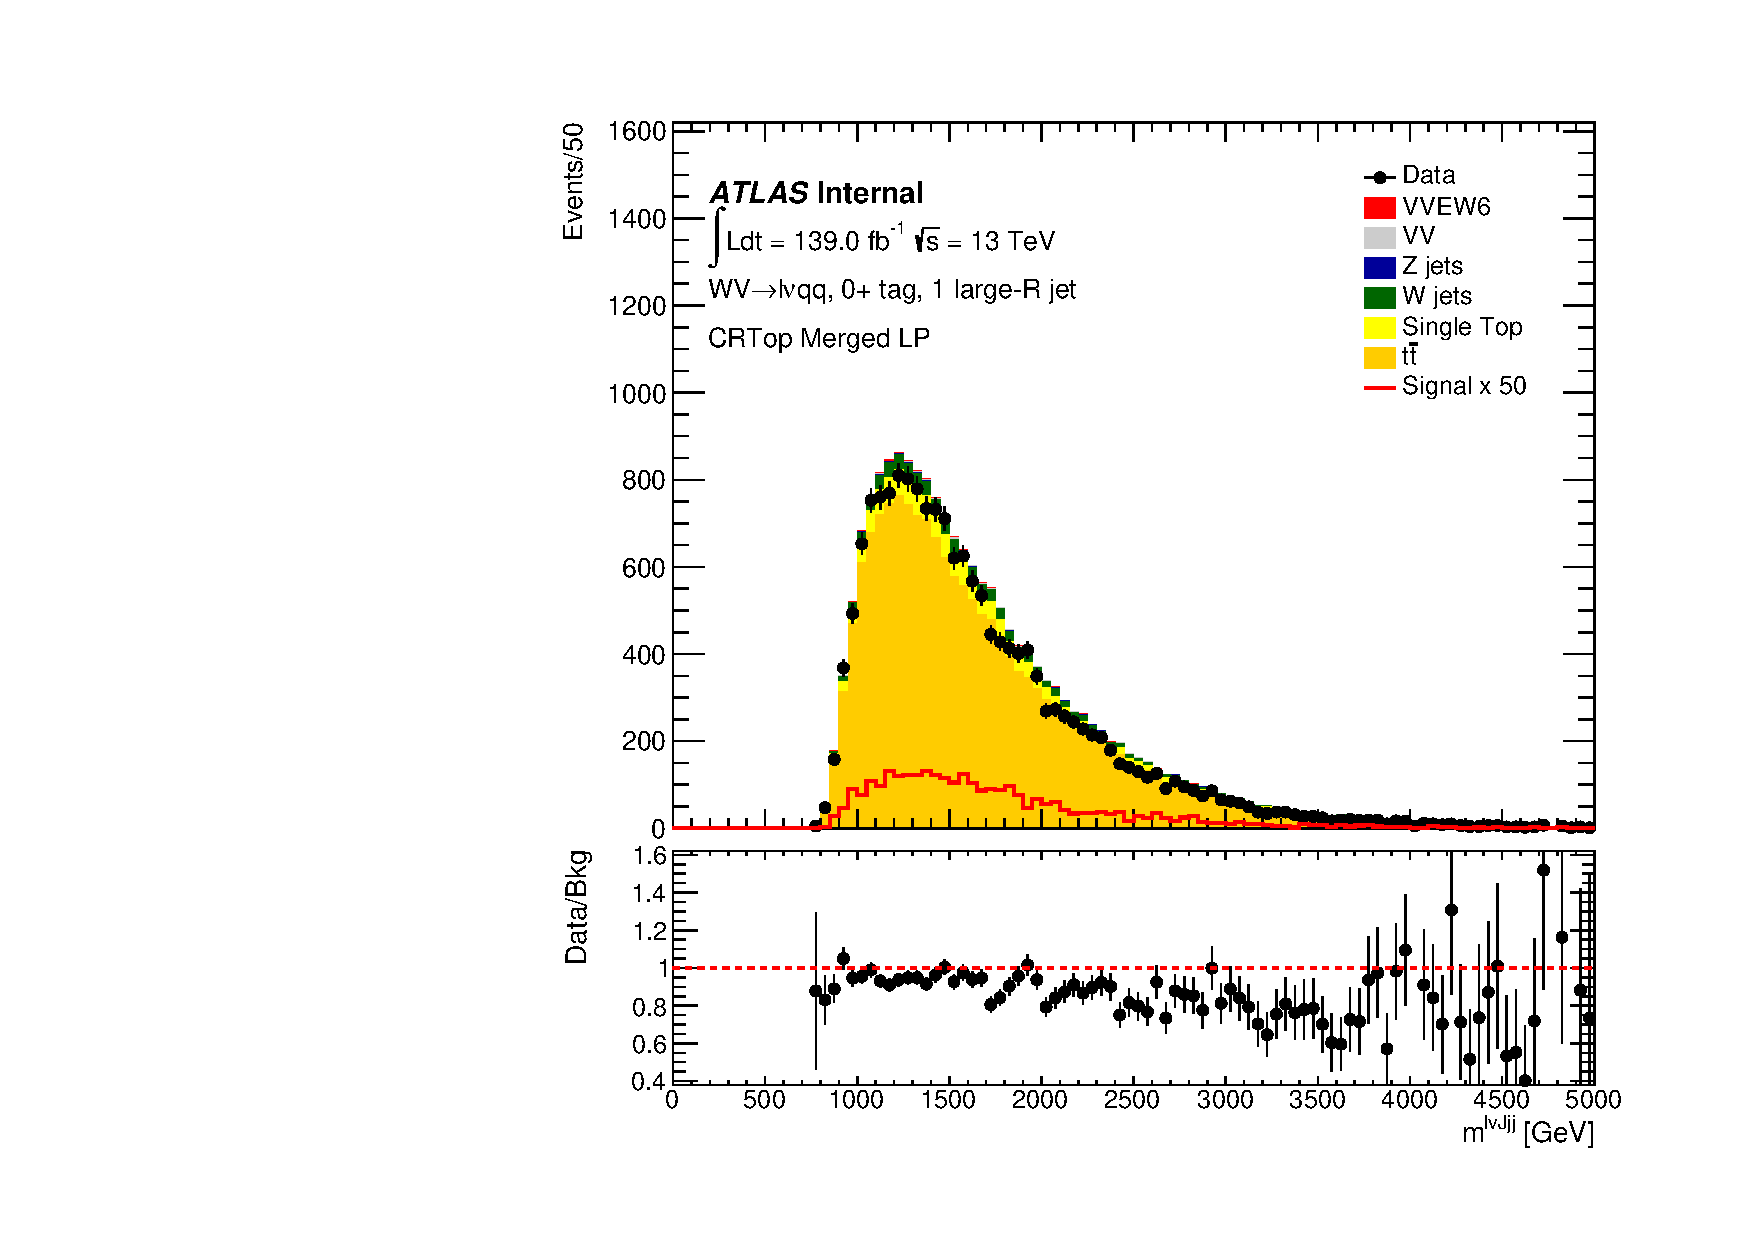
\includegraphics[width=0.3\textwidth]{figures/CRPlots/CRTop_80/stacked_plot_lvJjjmass.pdf}}
    \subfloat[]{\includegraphics[width=0.3\textwidth]{figures/CRPlots/CRTop_80/stacked_plot_lvJmass.pdf}} \\
    \caption{Data-MC checks for the merged low-purity top control region in the \olep channel.}
    \label{fig:CRTopMerLPPlots1Lep2}
\end{figure}

\begin{figure}[ht]
    \centering
    \subfloat[]{\includegraphics[width=0.3\textwidth]{figures/CRPlots/CRTop_50/stacked_plot_merged_tagMjj.pdf}}
    \subfloat[]{\includegraphics[width=0.3\textwidth]{figures/CRPlots/CRTop_50/stacked_plot_merged_tagJ1_pt.pdf}}
    \subfloat[]{\includegraphics[width=0.3\textwidth]{figures/CRPlots/CRTop_50/stacked_plot_merged_tagJ2_pt.pdf}} \\
    \subfloat[]{\includegraphics[width=0.3\textwidth]{figures/CRPlots/CRTop_50/stacked_plot_merged_tagJ1_eta.pdf}}
    \subfloat[]{\includegraphics[width=0.3\textwidth]{figures/CRPlots/CRTop_50/stacked_plot_merged_tagJ2_eta.pdf}} \\
    \subfloat[]{\includegraphics[width=0.3\textwidth]{figures/CRPlots/CRTop_50/stacked_plot_NJets.pdf}}
    \subfloat[]{\includegraphics[width=0.3\textwidth]{figures/CRPlots/CRTop_50/stacked_plot_NBJets.pdf}}
    \subfloat[]{\includegraphics[width=0.3\textwidth]{figures/CRPlots/CRTop_50/stacked_plot_lep_pt.pdf}} \\
    \subfloat[]{\includegraphics[width=0.3\textwidth]{figures/CRPlots/CRTop_50/stacked_plot_fatJ_m.pdf}}
    \subfloat[]{\includegraphics[width=0.3\textwidth]{figures/CRPlots/CRTop_50/stacked_plot_fatJ_pt.pdf}}
    \subfloat[]{\includegraphics[width=0.3\textwidth]{figures/CRPlots/CRTop_50/stacked_plot_fatJ_D2.pdf}}
    \caption{Data-MC checks for the merged high-purity top control region in the \olep channel.}
    \label{fig:CRTopMerHPPlots1Lep}
\end{figure}

\begin{figure}[ht]
    \centering
    \subfloat[]{\includegraphics[width=0.3\textwidth]{figures/CRPlots/CRTop_50/stacked_plot_W_m.pdf}}
    \subfloat[]{\includegraphics[width=0.3\textwidth]{figures/CRPlots/CRTop_50/stacked_plot_W_pt.pdf}}
    \subfloat[]{\includegraphics[width=0.3\textwidth]{figures/CRPlots/CRTop_50/stacked_plot_W_eta.pdf}} \\
    \subfloat[]{\includegraphics[width=0.3\textwidth]{figures/CRPlots/CRTop_50/stacked_plot_merged_tagJdEta.pdf}}
    \subfloat[]{\includegraphics[width=0.3\textwidth]{figures/CRPlots/CRTop_50/stacked_plot_fatJ_dRj1.pdf}}
    \subfloat[]{\includegraphics[width=0.3\textwidth]{figures/CRPlots/CRTop_50/stacked_plot_fatJ_dRj2.pdf}} \\
    \subfloat[]{\includegraphics[width=0.3\textwidth]{figures/CRPlots/CRTop_50/stacked_plot_lvJjjmass.pdf}}
    \subfloat[]{\includegraphics[width=0.3\textwidth]{figures/CRPlots/CRTop_50/stacked_plot_lvJmass.pdf}} \\
    \caption{Data-MC checks for the merged high-purity top control region in the \olep channel.}
    \label{fig:CRTopMerHPPlots1Lep2}
\end{figure}

%%%%%%%%%%
